\clearpage\section{Selected 2024 supporting distributions}\label{app:2024-support}
The following distributions document the efficiency inputs, statistical precision, and uncertainty composition for the 2024 measurement. Only inclusive distributions directly related to the correction or its principal checks are selected. The jet- and vertex-split variants and the full set of individual-jet and angular distributions are not reproduced. These plots use the measurement sample and are not independent closure tests.
\subsection{$ee$ channel}
\begin{figure}[htbp]\centering
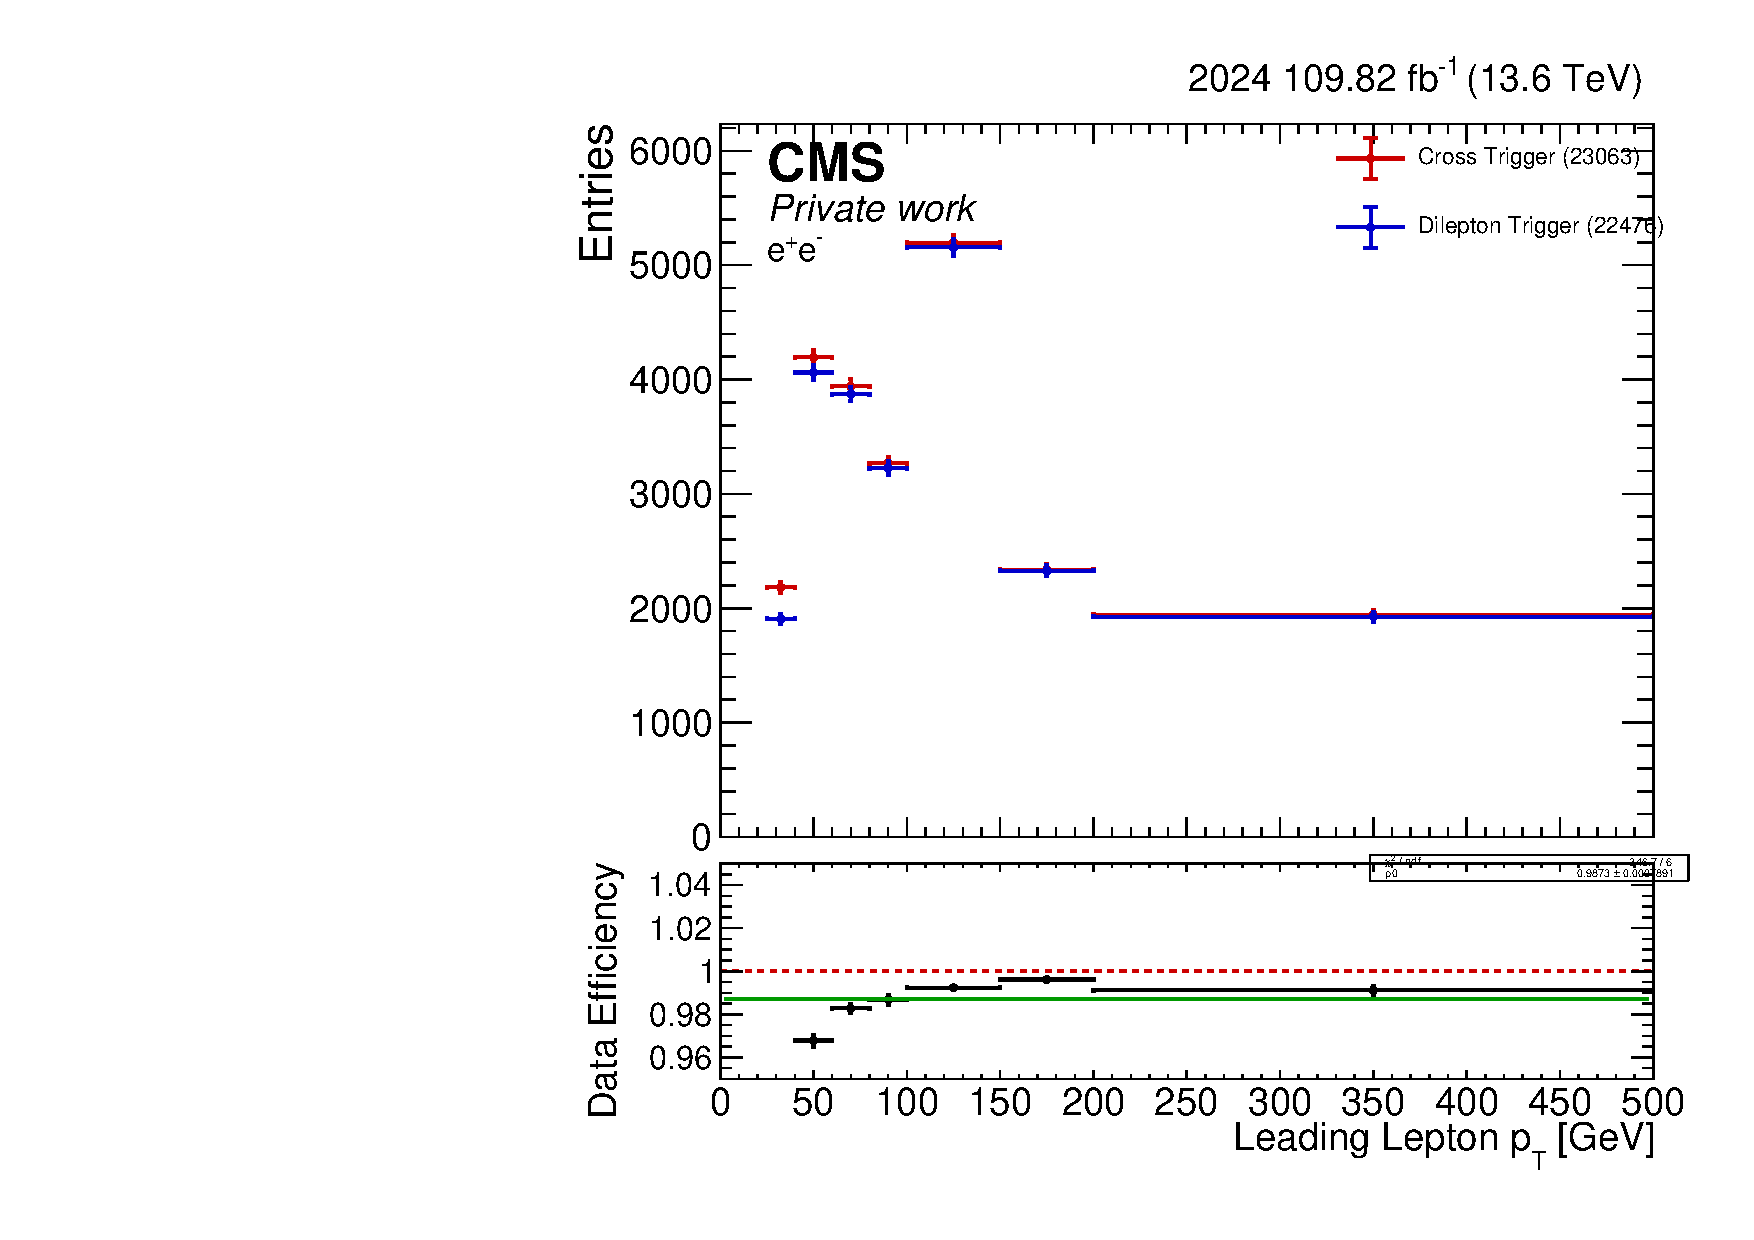
\includegraphics[width=0.48\linewidth]{figures/2024/ElEl/TrigEffData/TrigEff_Lep1pt.pdf}
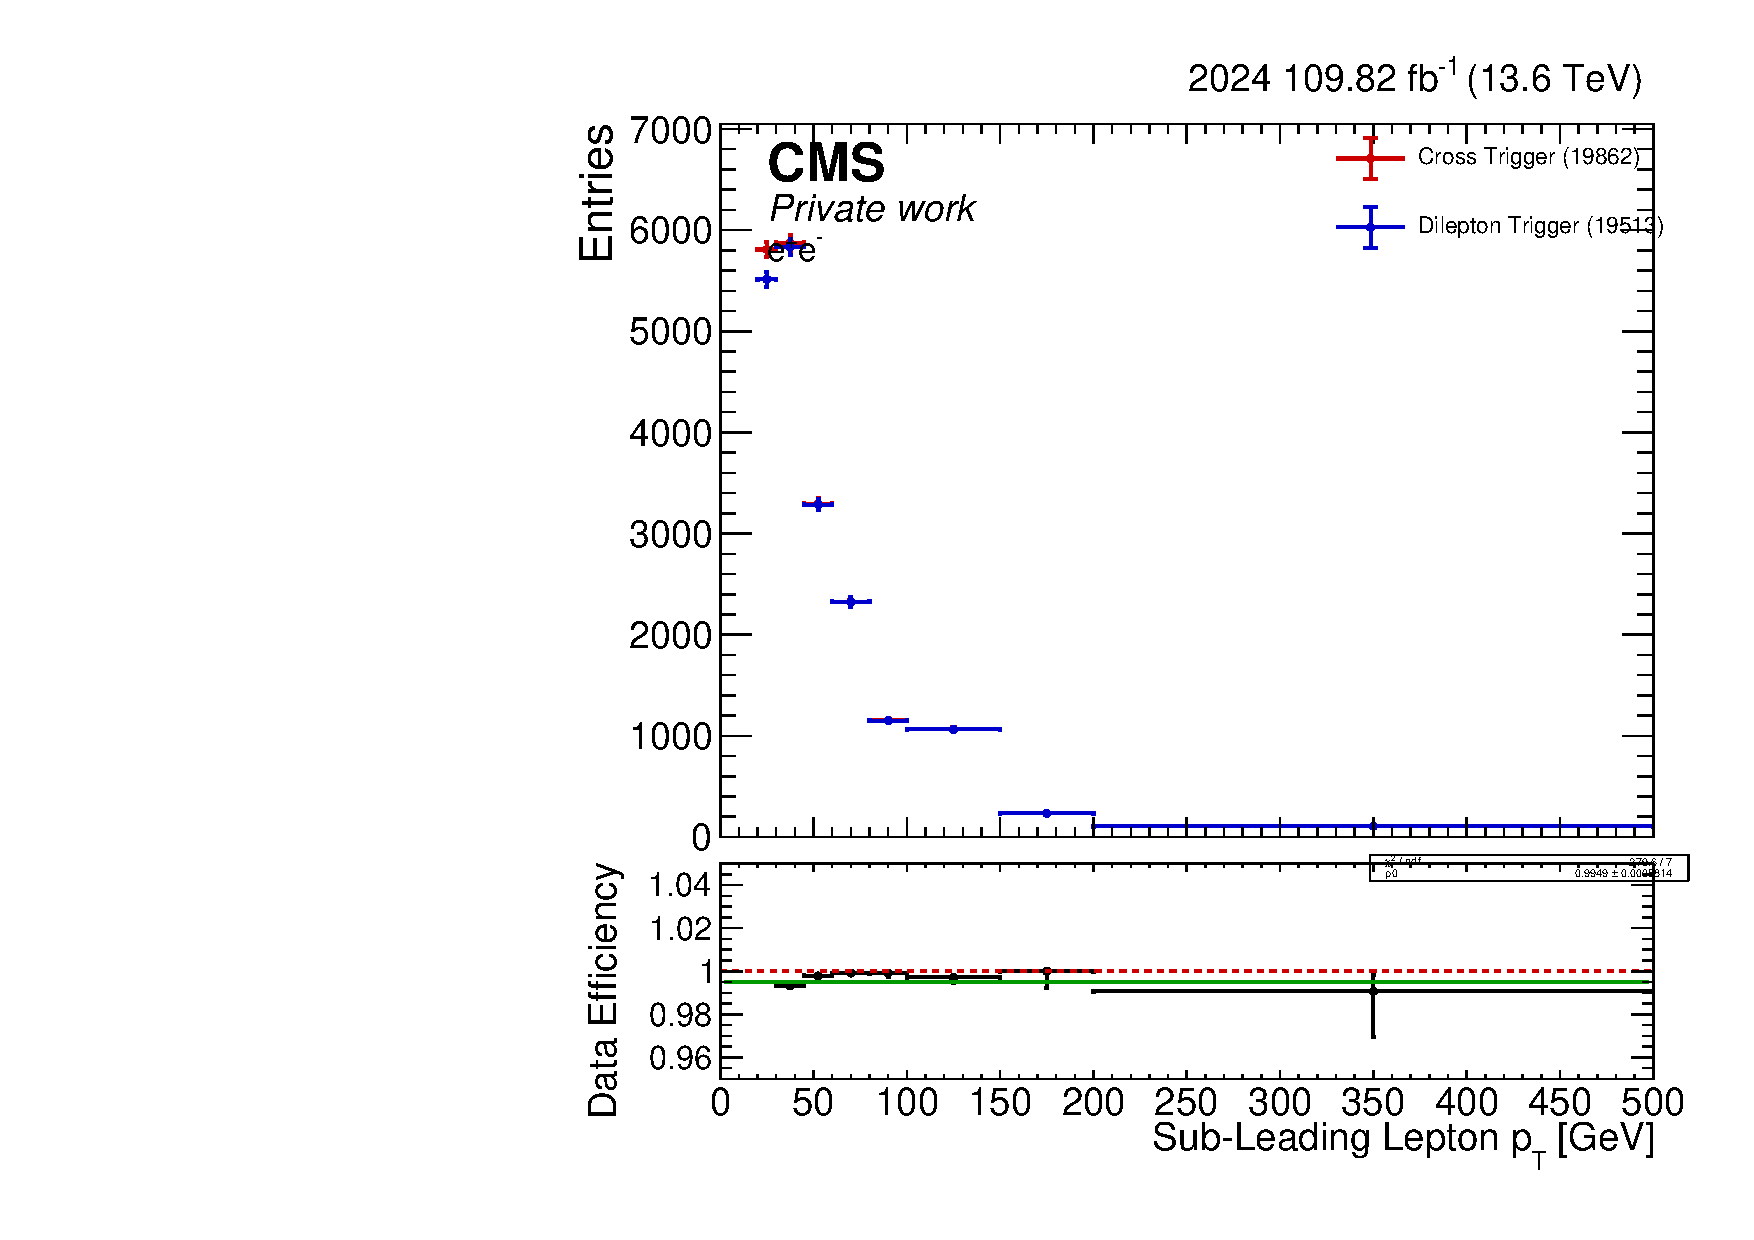
\includegraphics[width=0.48\linewidth]{figures/2024/ElEl/TrigEffData/TrigEff_Lep2pt.pdf}
\caption{Data trigger numerator and reference-sample distributions (upper panels), with their efficiency ratios (lower panels) in the $ee$ channel. Left and right: leading and subleading lepton $p_{\mathrm{T}}$.}\label{fig:extra-ElEl-TrigEffData-Lep1pt}\end{figure}
\begin{figure}[p]\centering
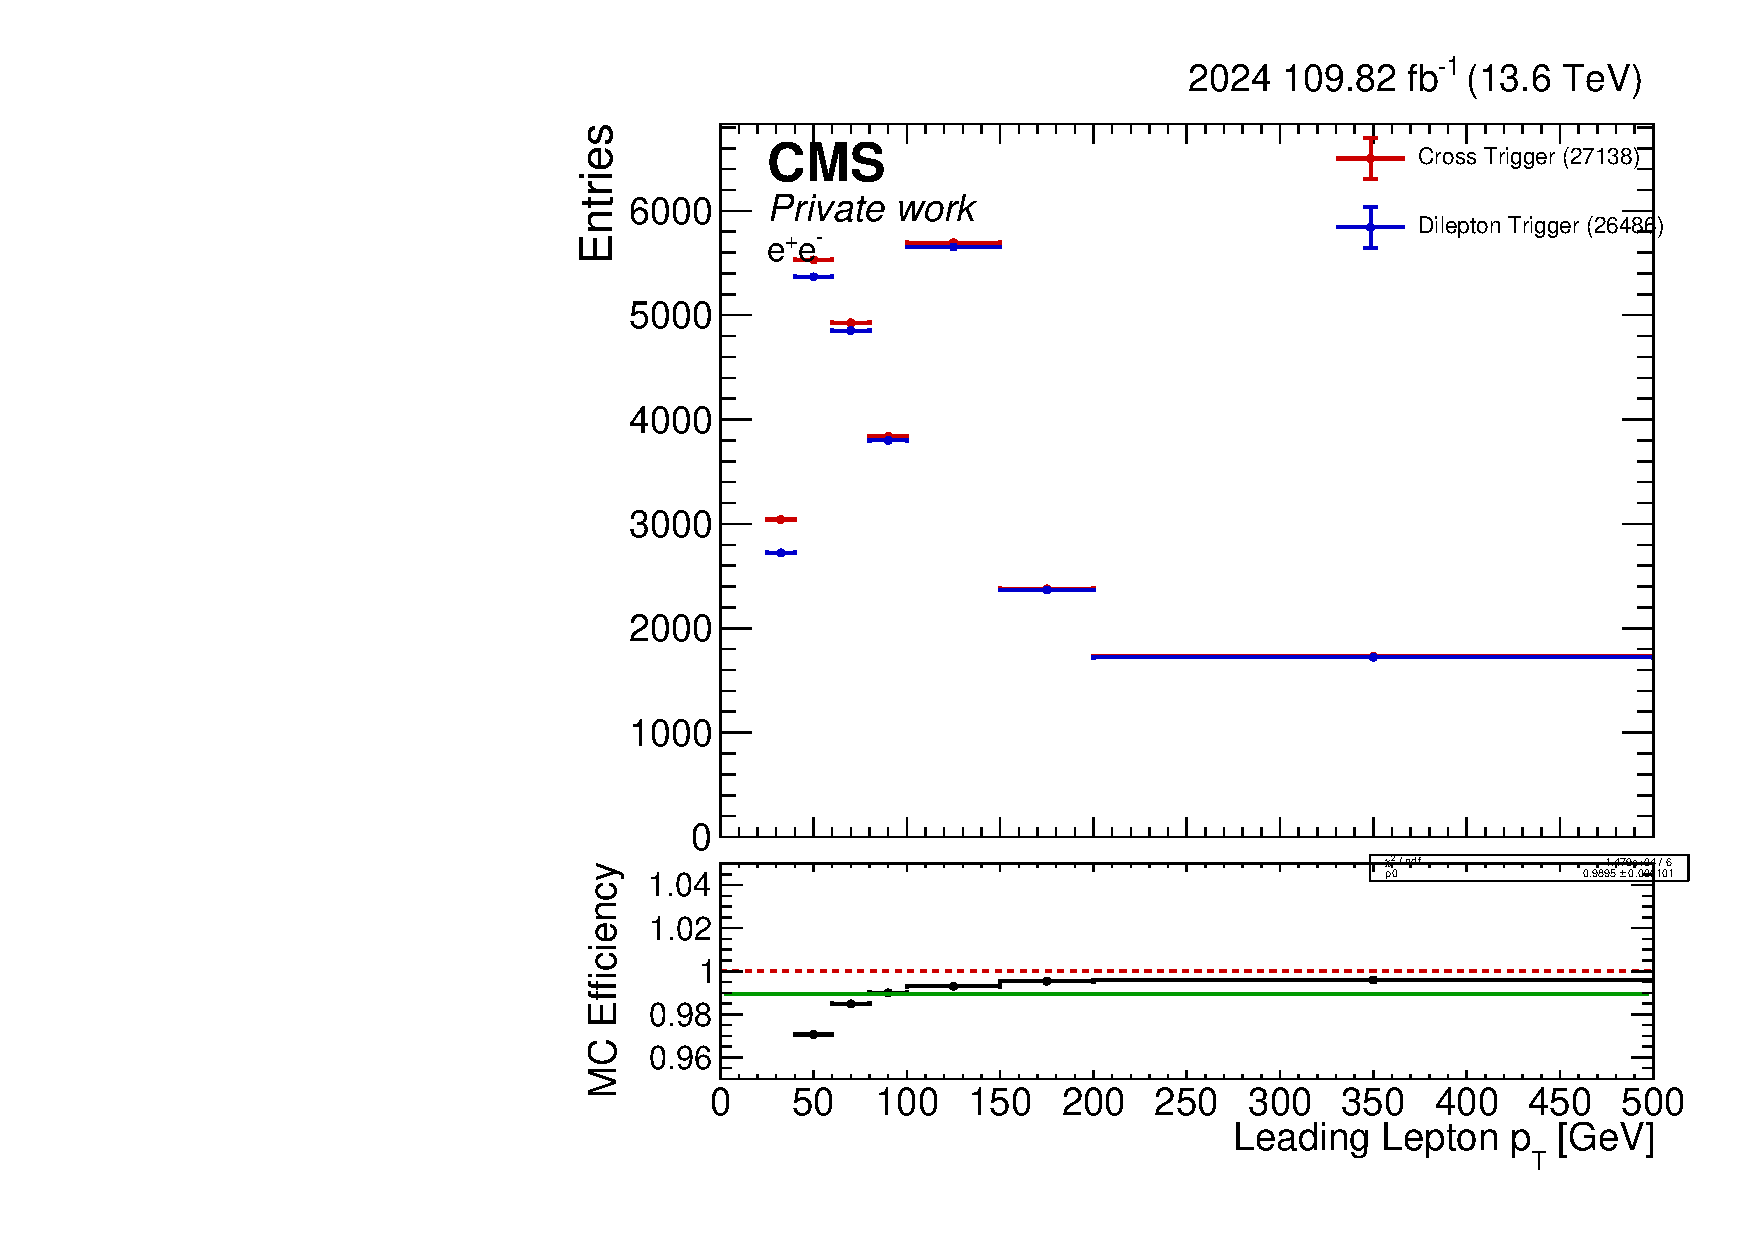
\includegraphics[width=0.48\linewidth]{figures/2024/ElEl/TrigEffMC/TrigEff_Lep1pt.pdf}
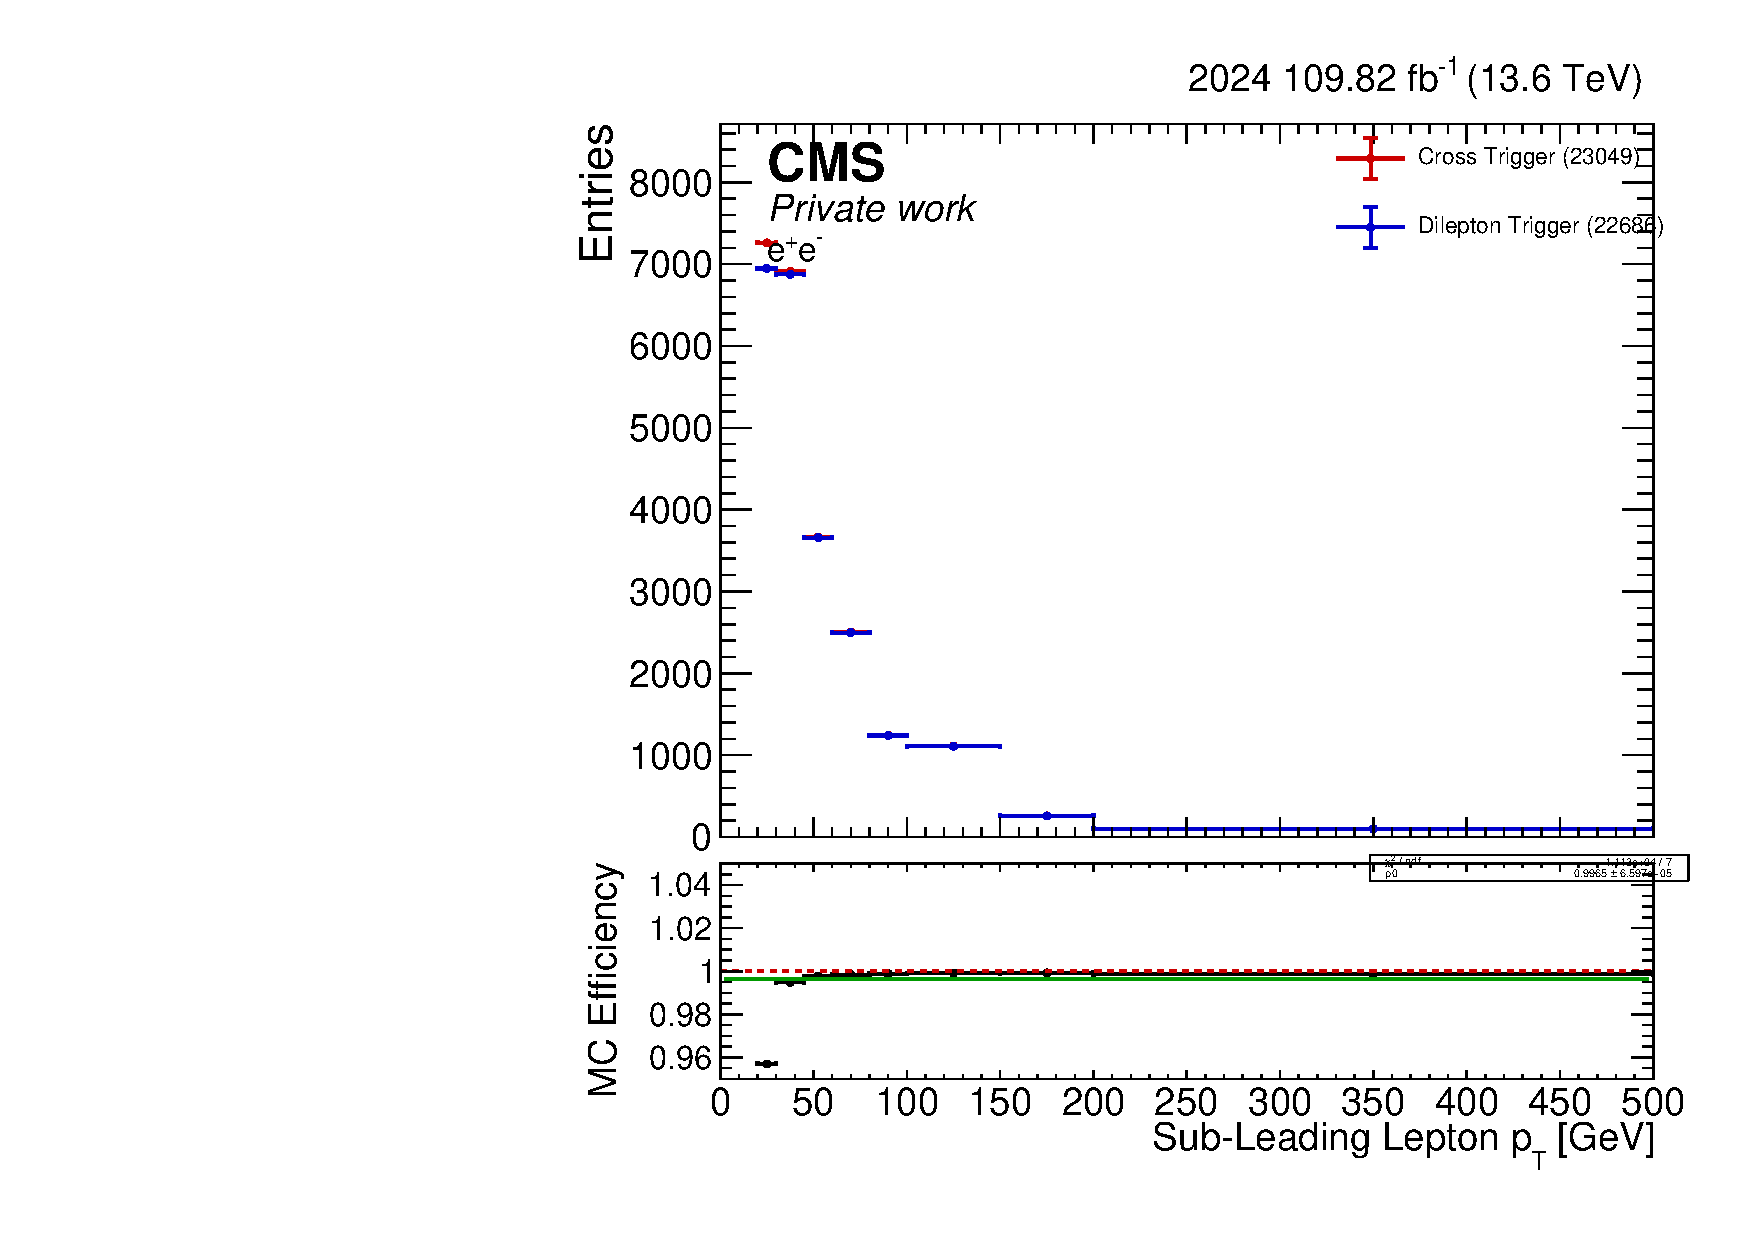
\includegraphics[width=0.48\linewidth]{figures/2024/ElEl/TrigEffMC/TrigEff_Lep2pt.pdf}
\caption{Simulated trigger numerator and reference-sample distributions (upper panels), with their efficiency ratios (lower panels) in the $ee$ channel. Left and right: leading and subleading lepton $p_{\mathrm{T}}$.}\label{fig:extra-ElEl-TrigEffMC-Lep1pt}\end{figure}
\begin{figure}[p]\centering
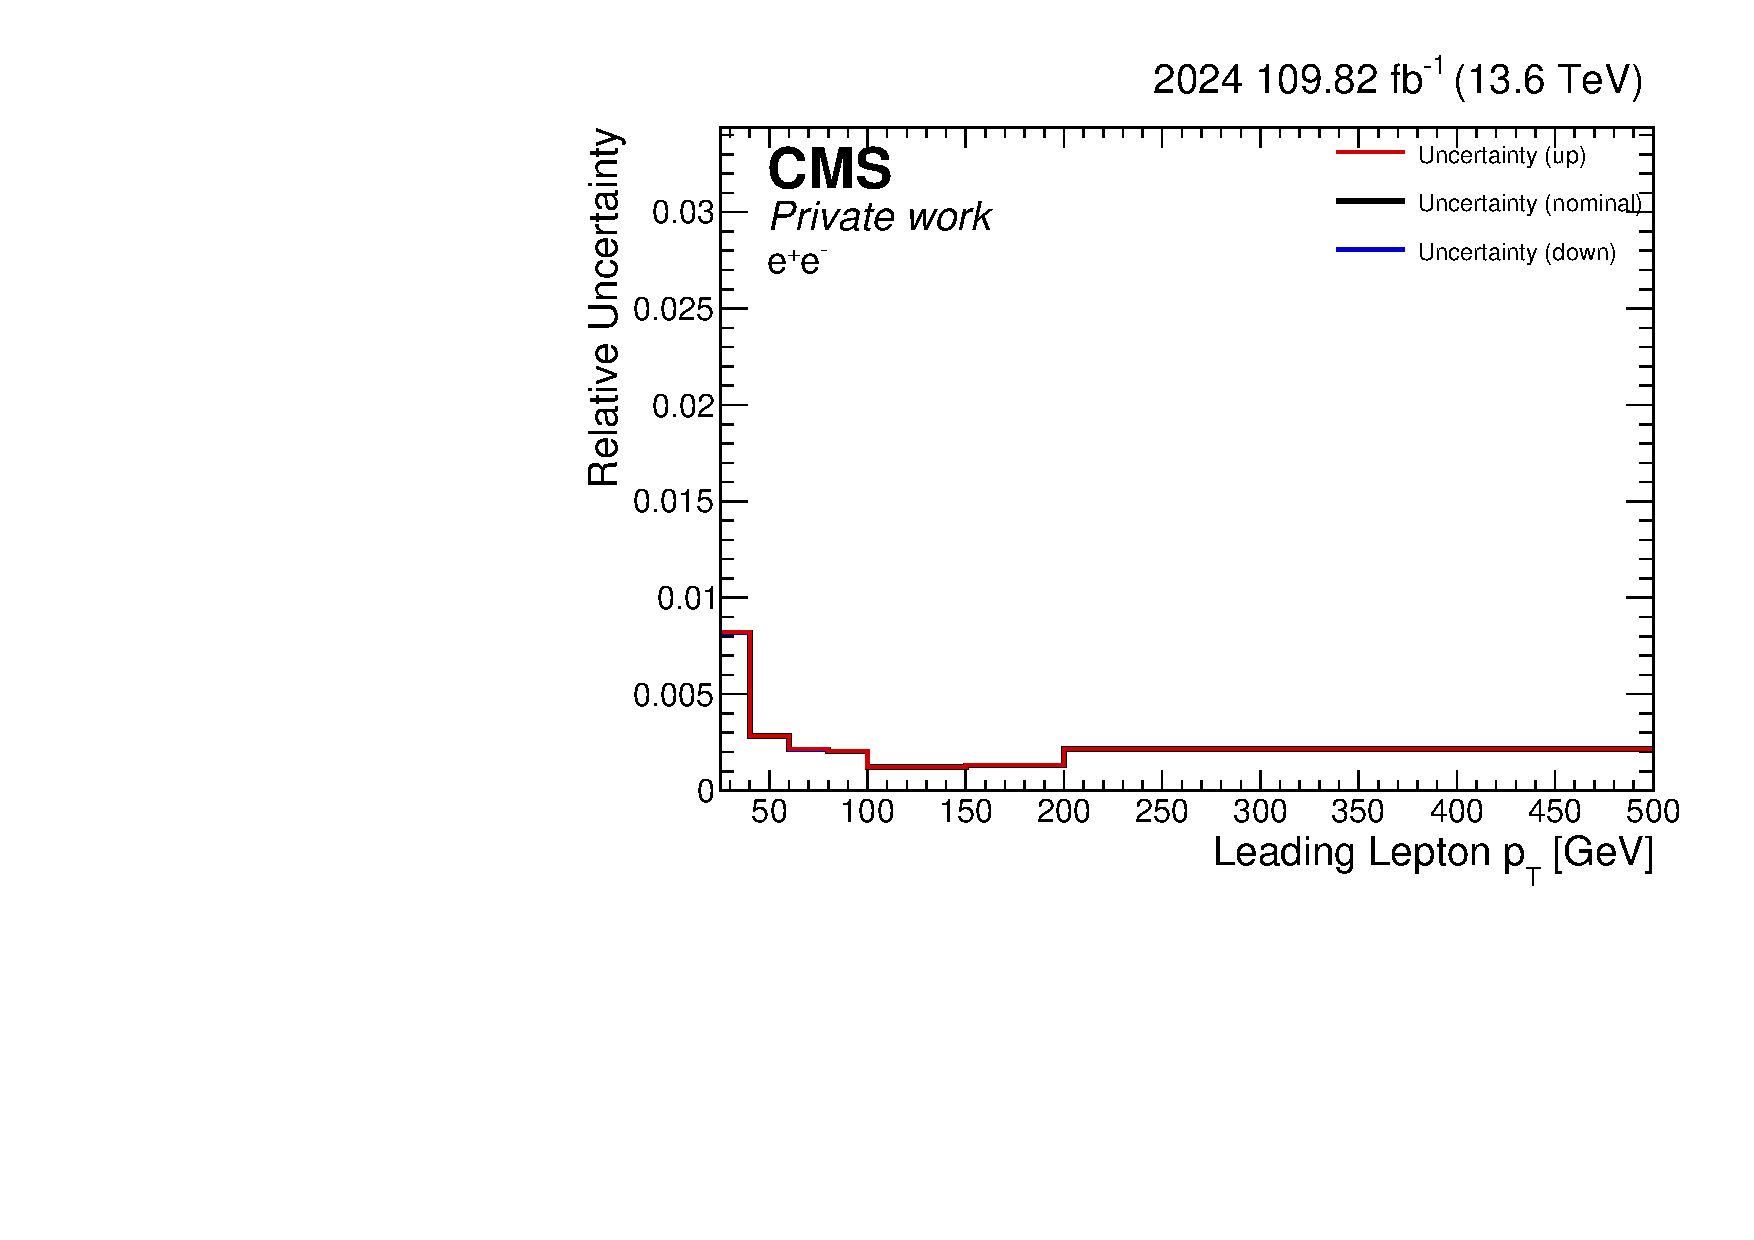
\includegraphics[width=0.48\linewidth]{figures/2024/ElEl/Statistical_Uncertainty/UncRatio_Lep1pt.pdf}
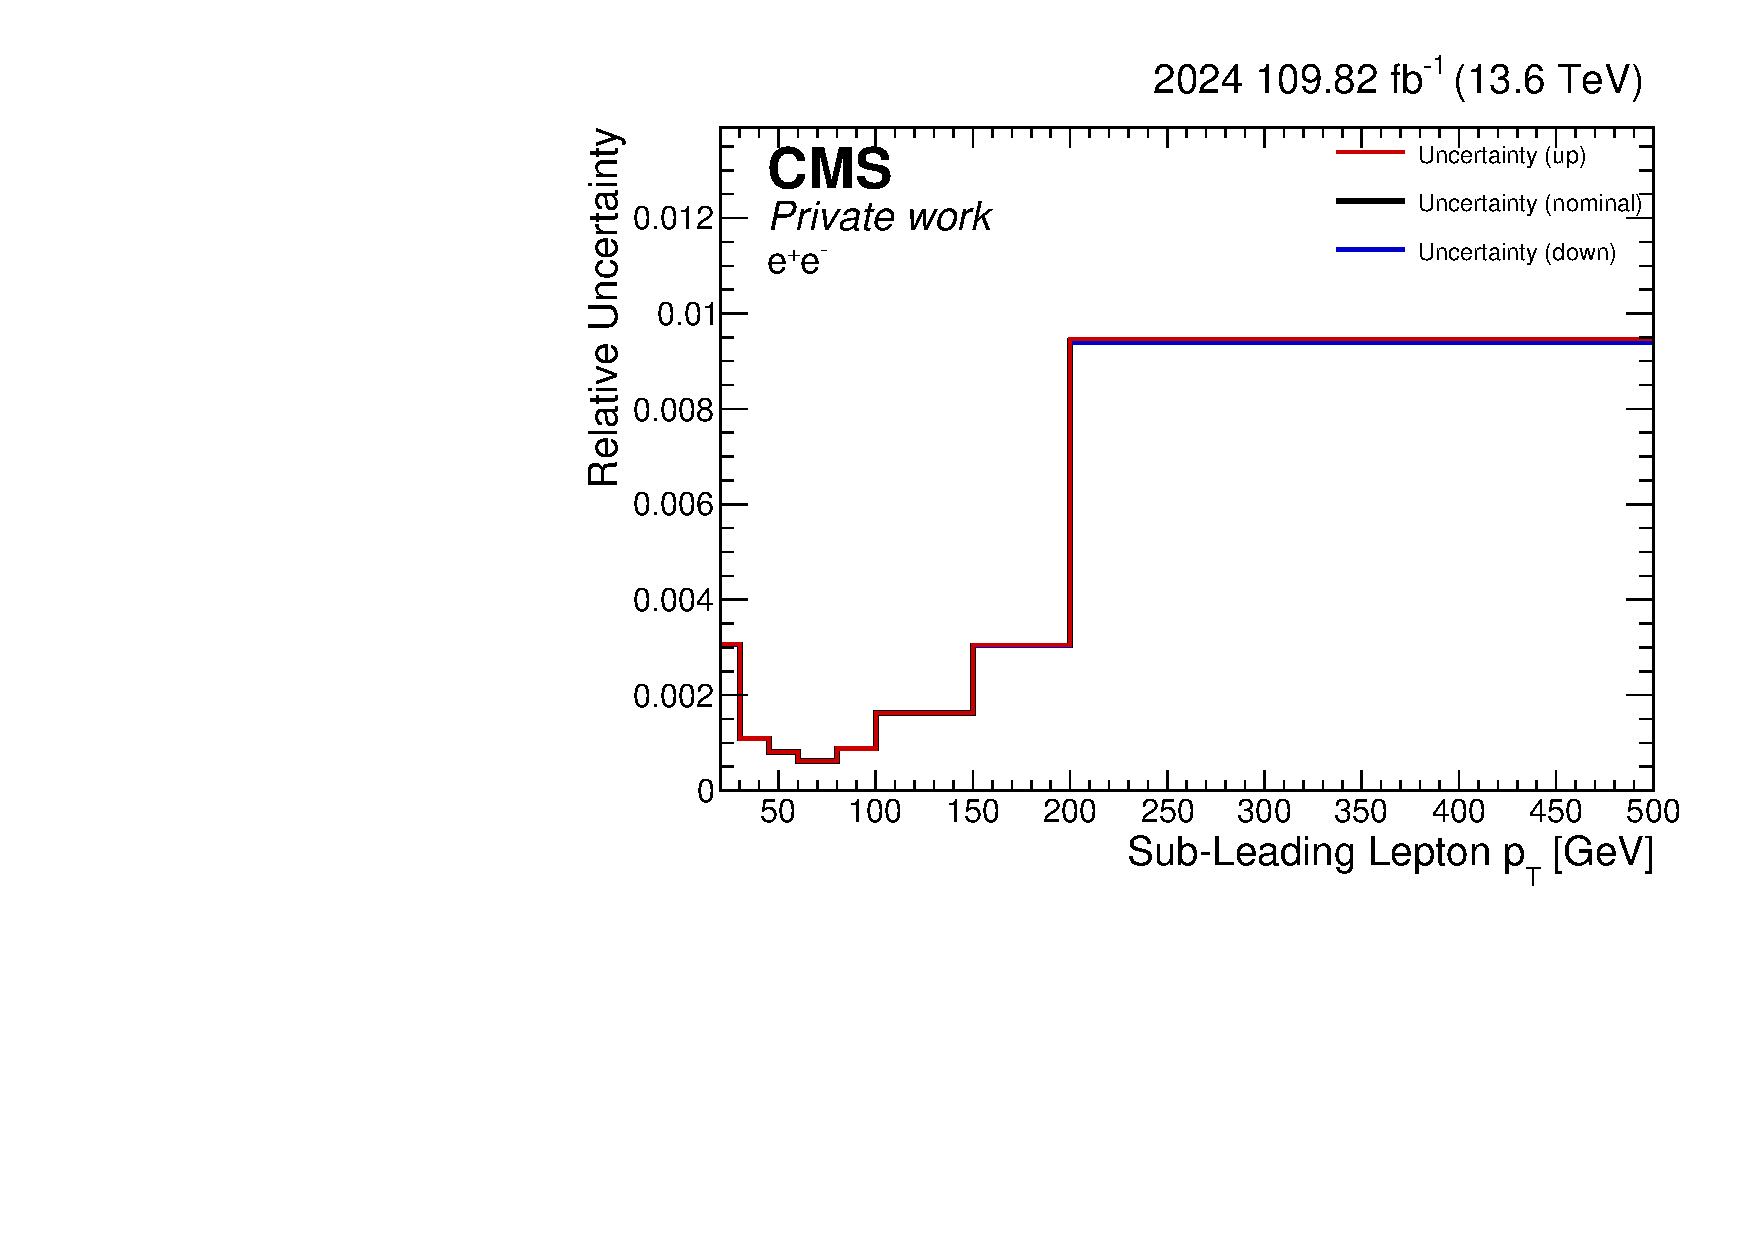
\includegraphics[width=0.48\linewidth]{figures/2024/ElEl/Statistical_Uncertainty/UncRatio_Lep2pt.pdf}
\caption{Relative statistical uncertainty diagnostics, retaining the nominal, upward, and downward curves of the supplied production in the $ee$ channel. Left and right: leading and subleading lepton $p_{\mathrm{T}}$.}\label{fig:extra-ElEl-Statistical-Uncertainty-Lep1pt}\end{figure}
\begin{figure}[p]\centering
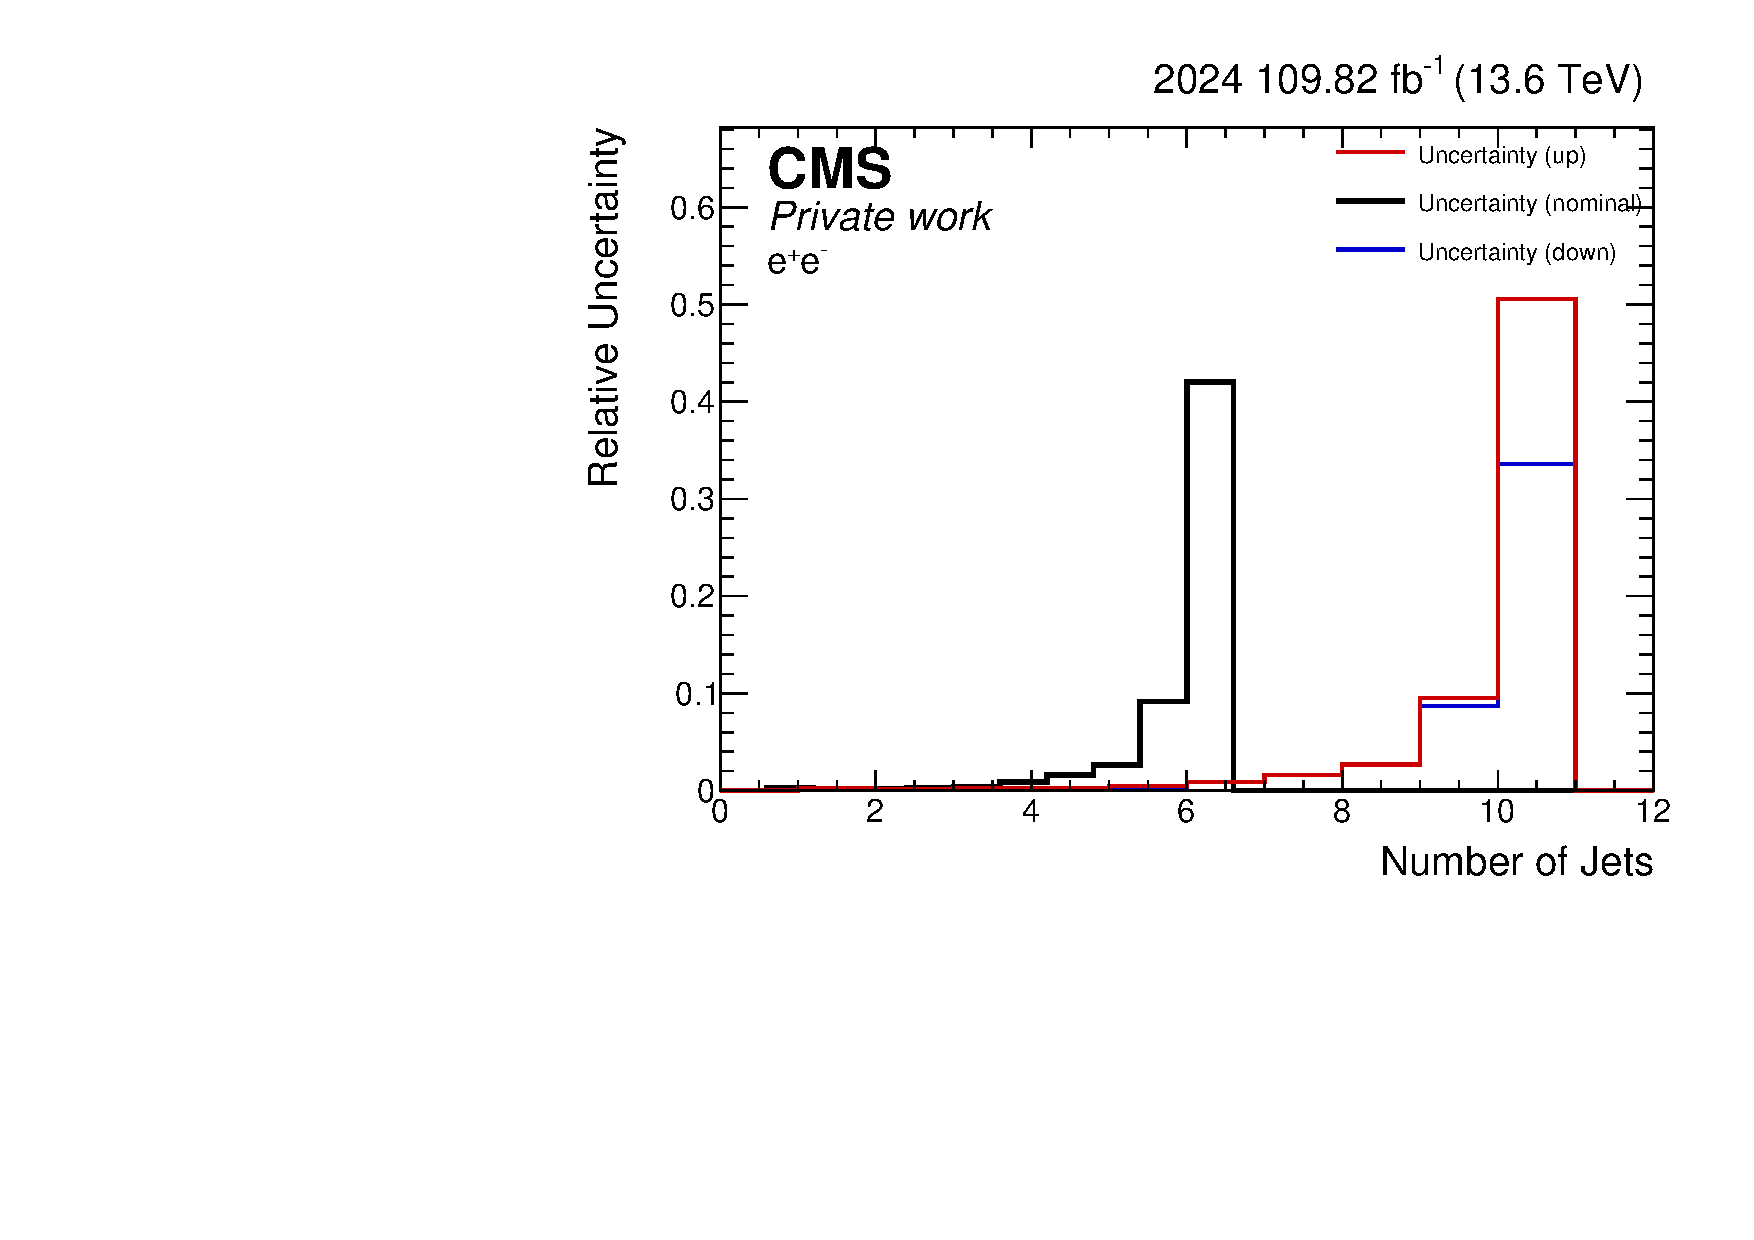
\includegraphics[width=0.48\linewidth]{figures/2024/ElEl/Statistical_Uncertainty/UncRatio_Num_Jets.pdf}
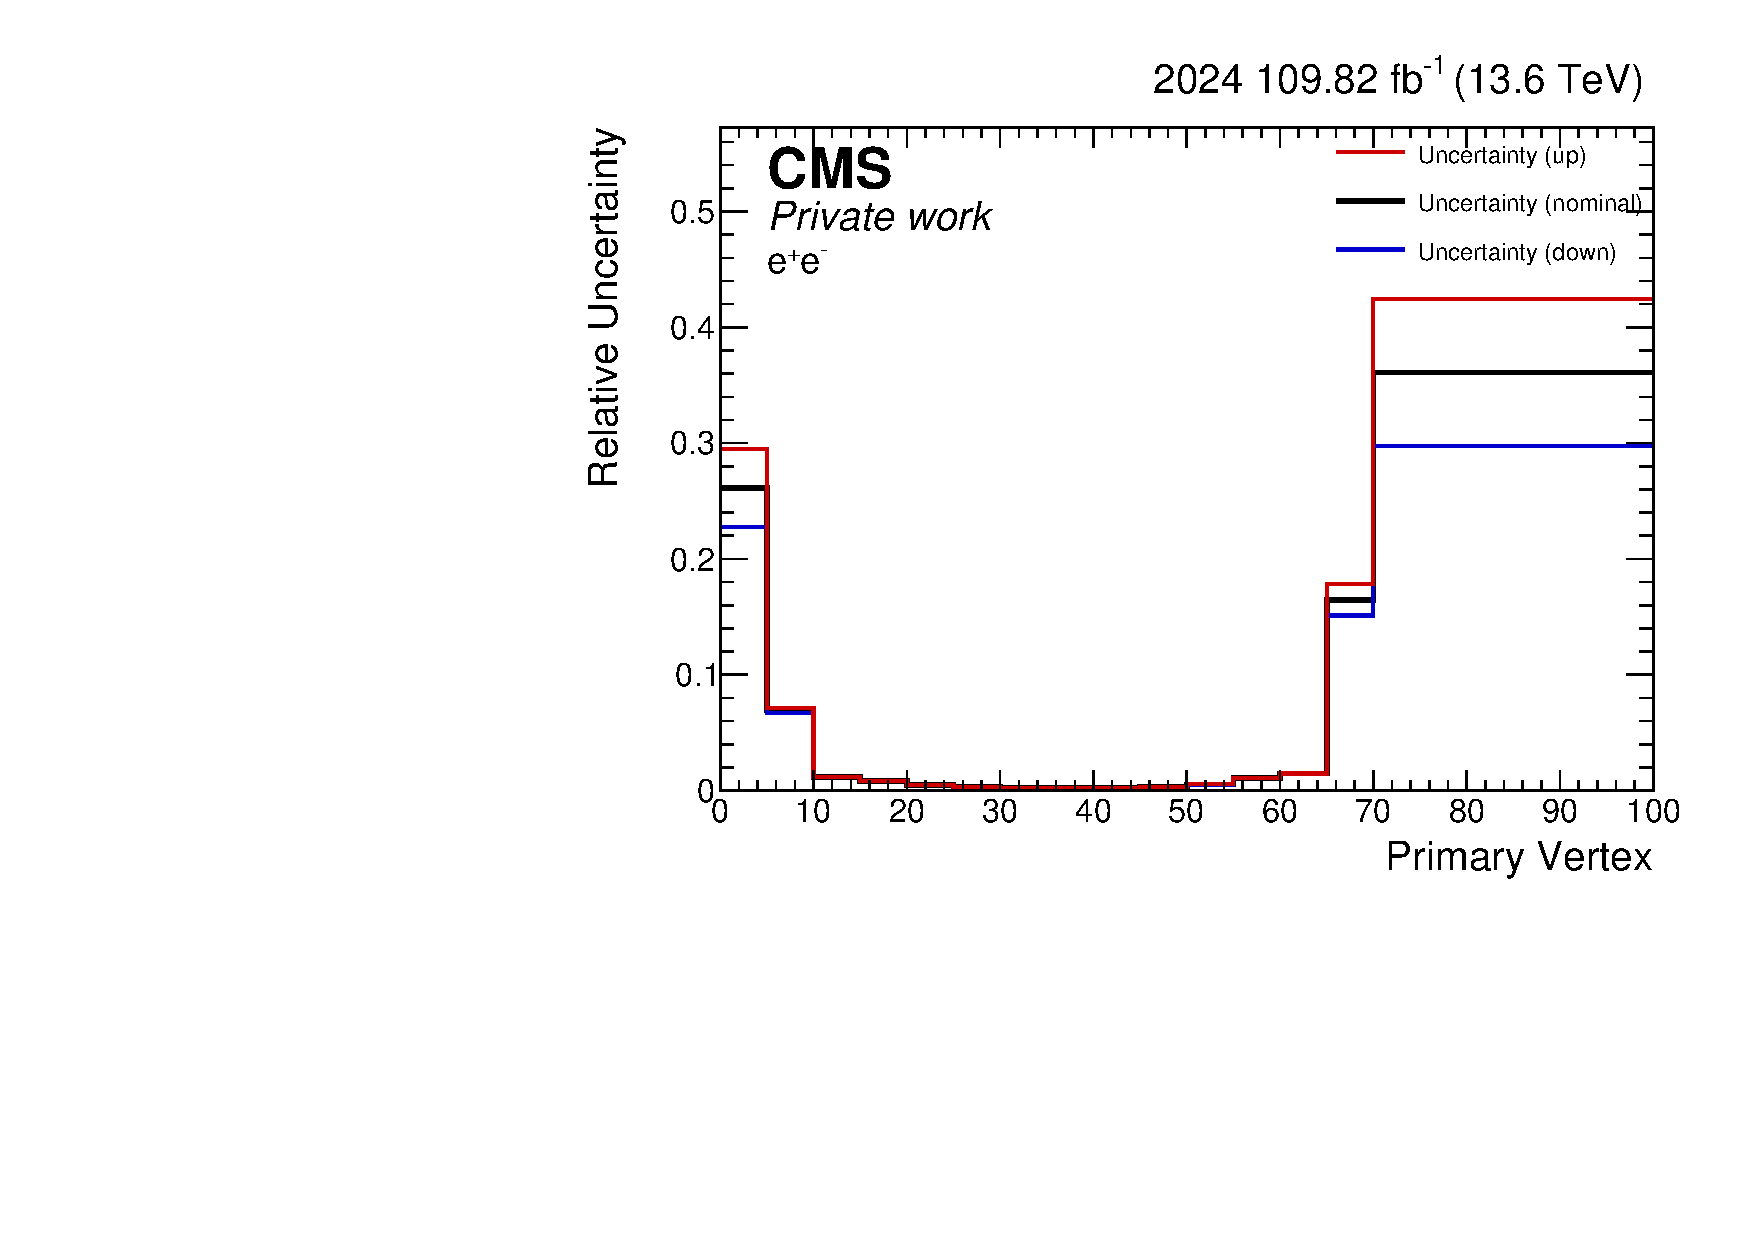
\includegraphics[width=0.48\linewidth]{figures/2024/ElEl/Statistical_Uncertainty/UncRatio_Num_PV.pdf}
\caption{Relative statistical uncertainty diagnostics, retaining the nominal, upward, and downward curves of the supplied production in the $ee$ channel. Left and right: jet and primary-vertex multiplicities.}\label{fig:extra-ElEl-Statistical-Uncertainty-Num_Jets}\end{figure}
\begin{figure}[p]\centering
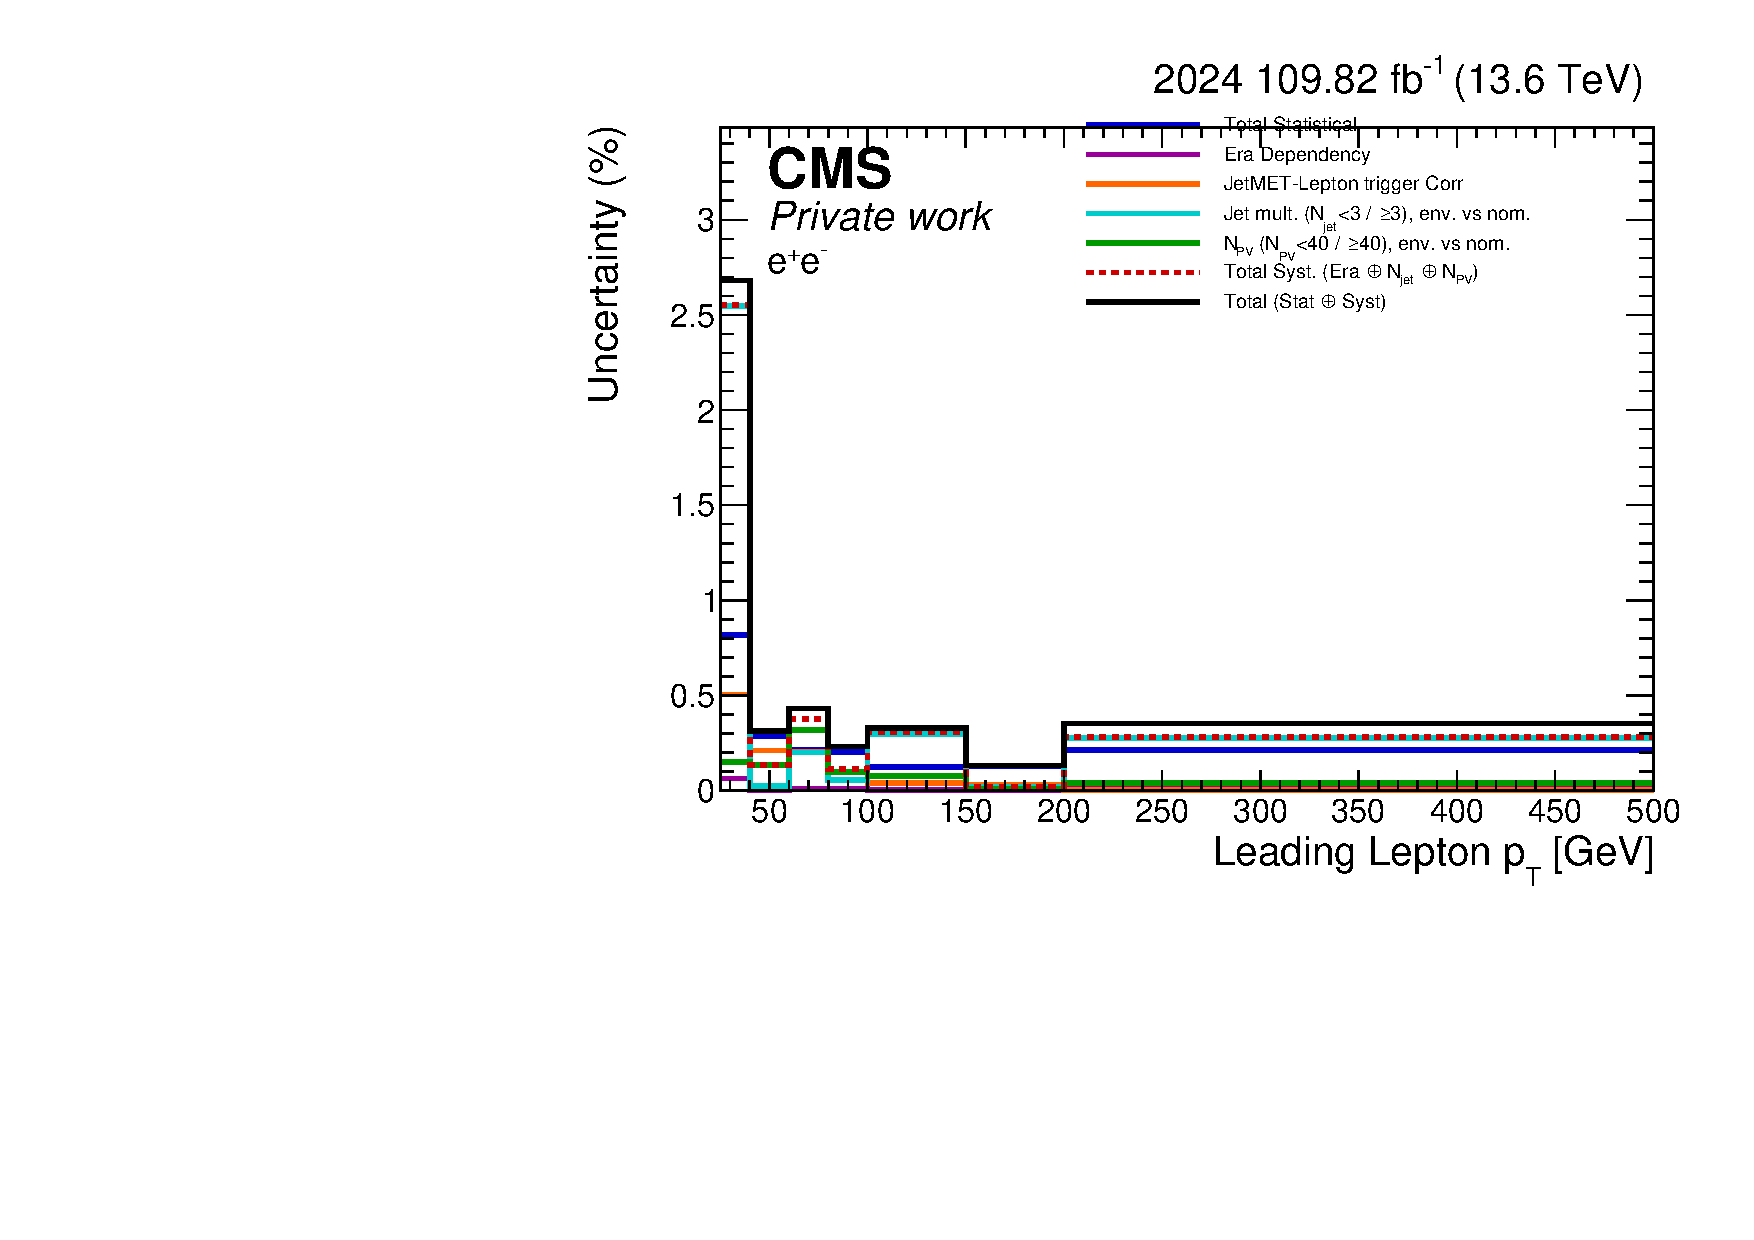
\includegraphics[width=0.48\linewidth]{figures/2024/ElEl/Uncertainty_Breakdown/Breakdown_Lep1pt.pdf}
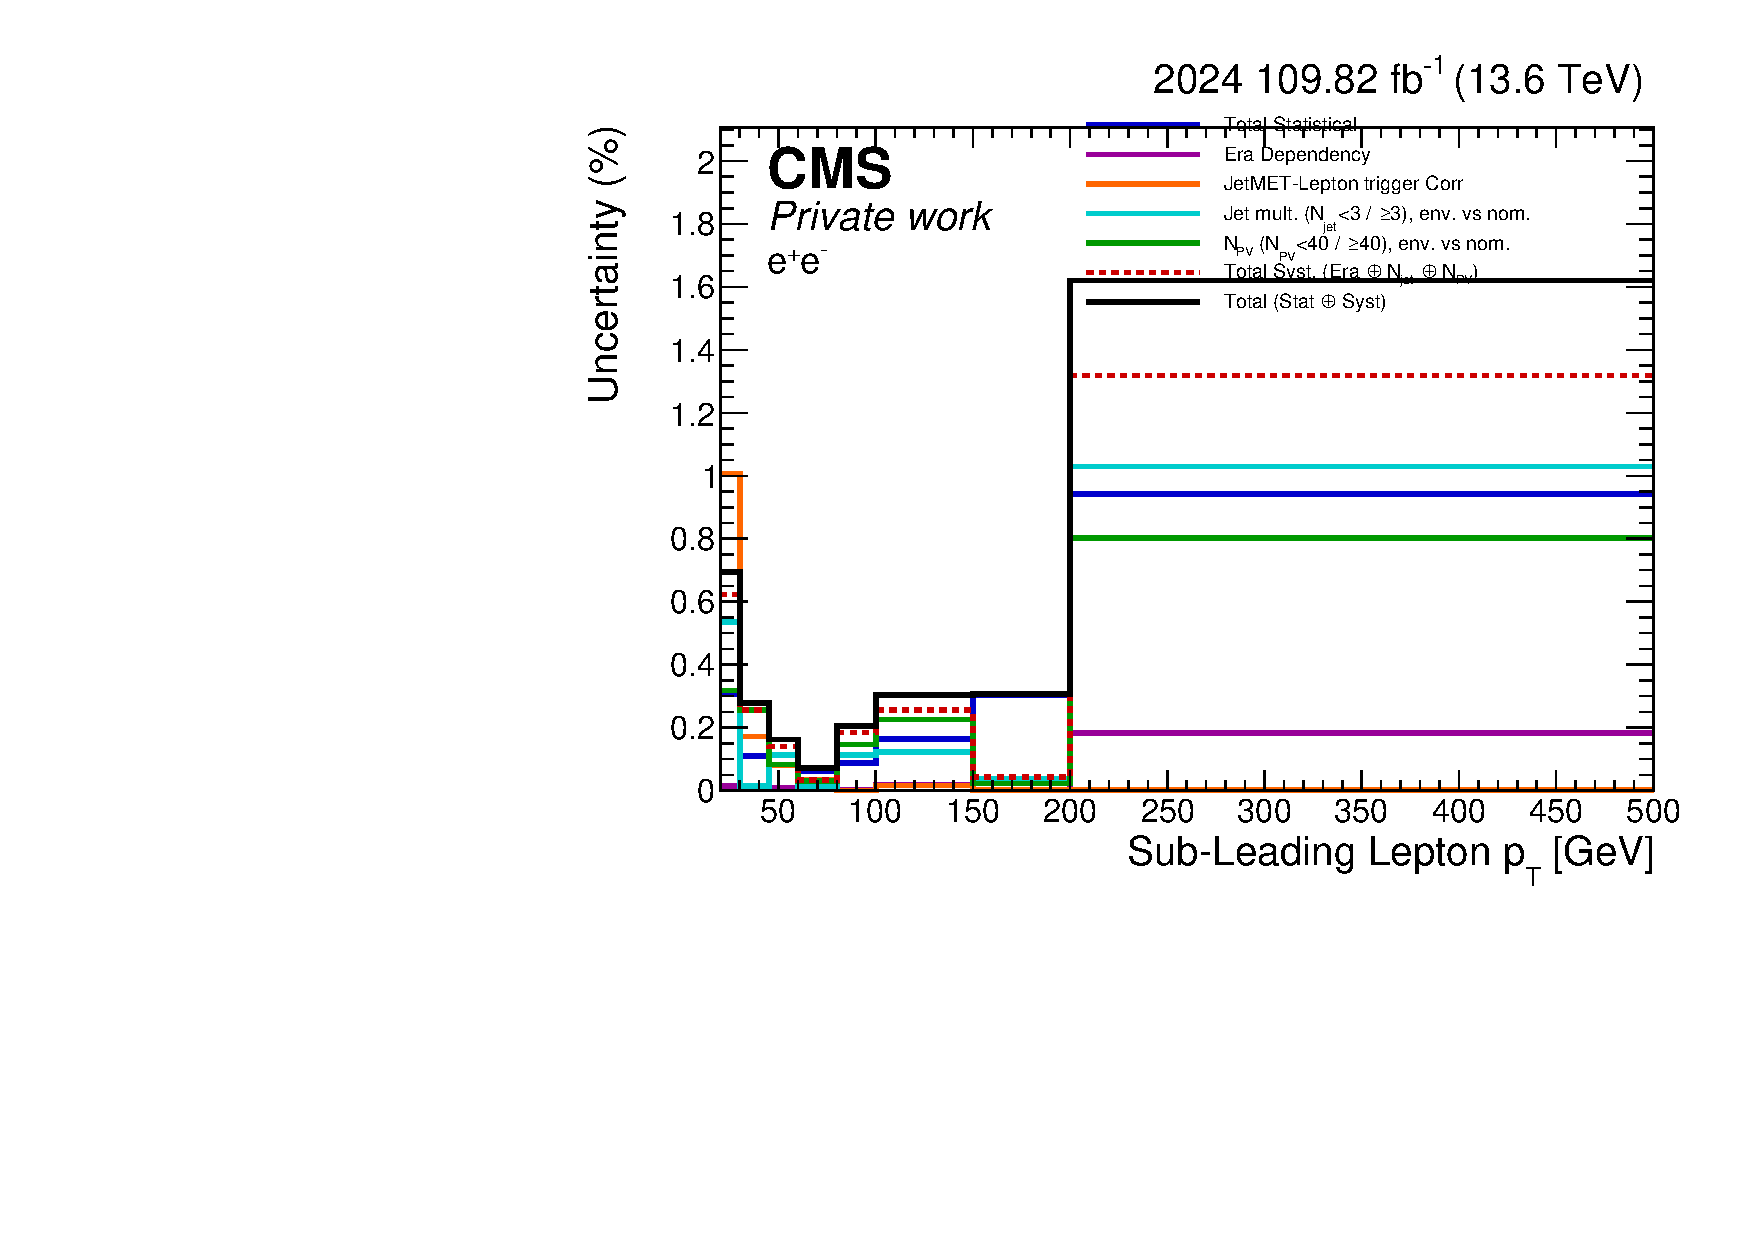
\includegraphics[width=0.48\linewidth]{figures/2024/ElEl/Uncertainty_Breakdown/Breakdown_Lep2pt.pdf}
\caption{Absolute uncertainty component breakdown in the $ee$ channel. Left and right: leading and subleading lepton $p_{\mathrm{T}}$.}\label{fig:extra-ElEl-Uncertainty-Breakdown-Lep1pt}\end{figure}
\begin{figure}[p]\centering
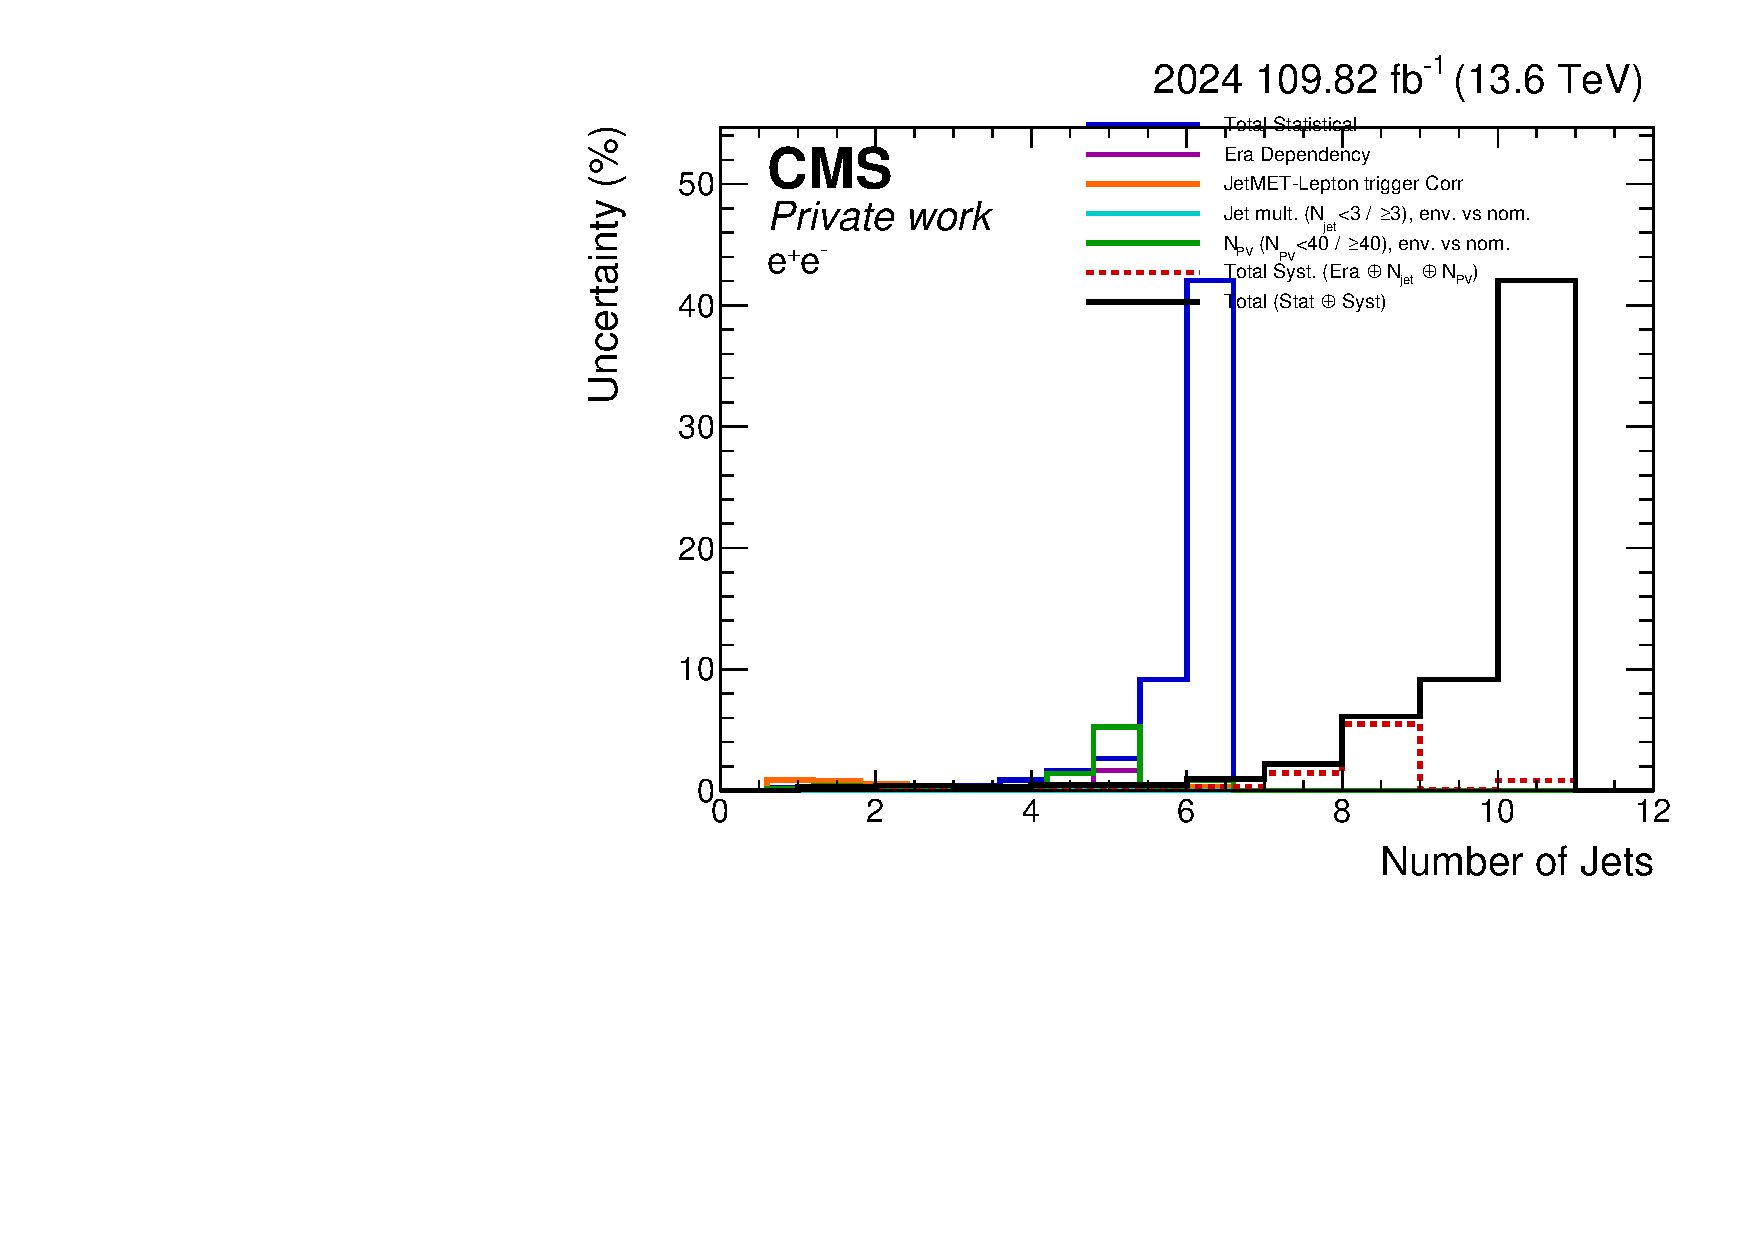
\includegraphics[width=0.48\linewidth]{figures/2024/ElEl/Uncertainty_Breakdown/Breakdown_Num_Jets.pdf}
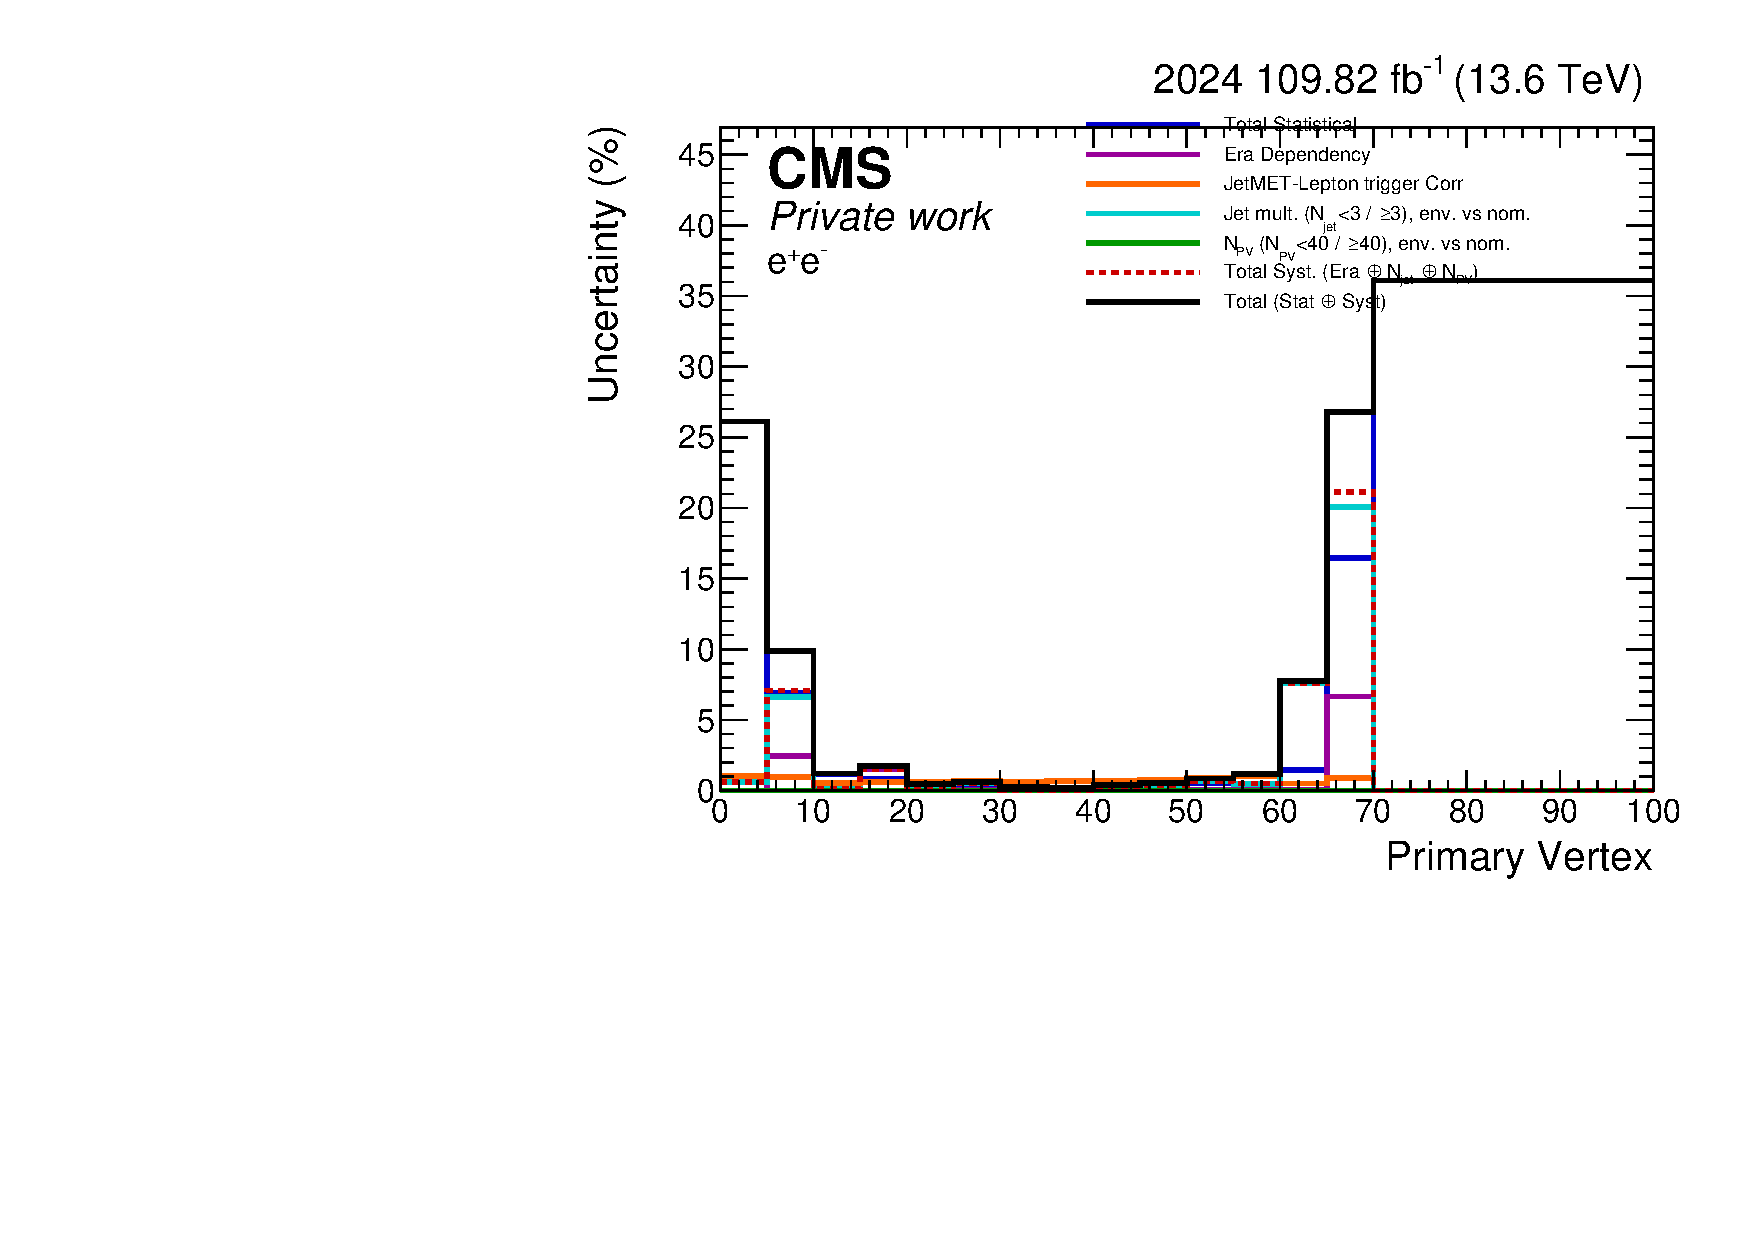
\includegraphics[width=0.48\linewidth]{figures/2024/ElEl/Uncertainty_Breakdown/Breakdown_Num_PV.pdf}
\caption{Absolute uncertainty component breakdown in the $ee$ channel. Left and right: jet and primary-vertex multiplicities.}\label{fig:extra-ElEl-Uncertainty-Breakdown-Num_Jets}\end{figure}
\begin{figure}[p]\centering
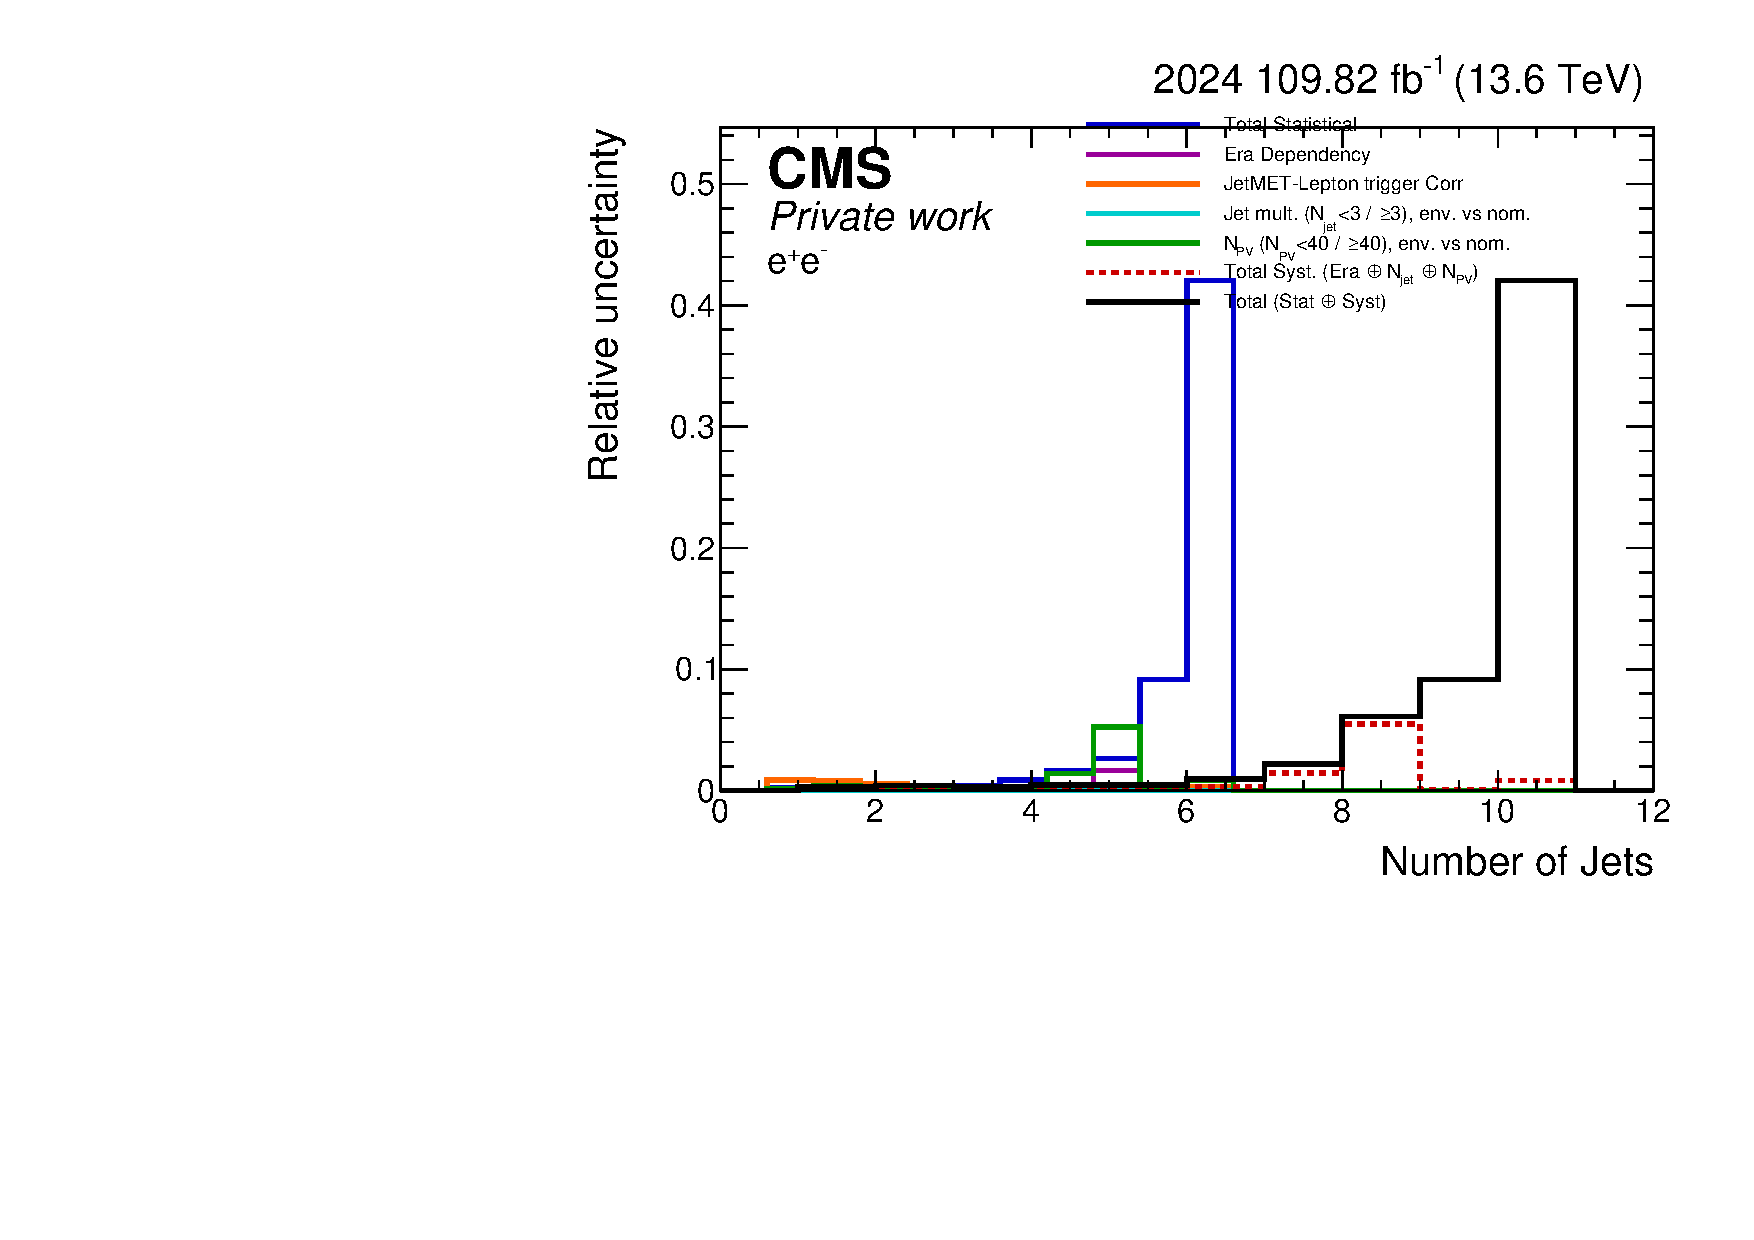
\includegraphics[width=0.48\linewidth]{figures/2024/ElEl/Relative_Uncertainty_Breakdown/Breakdown_Num_Jets.pdf}
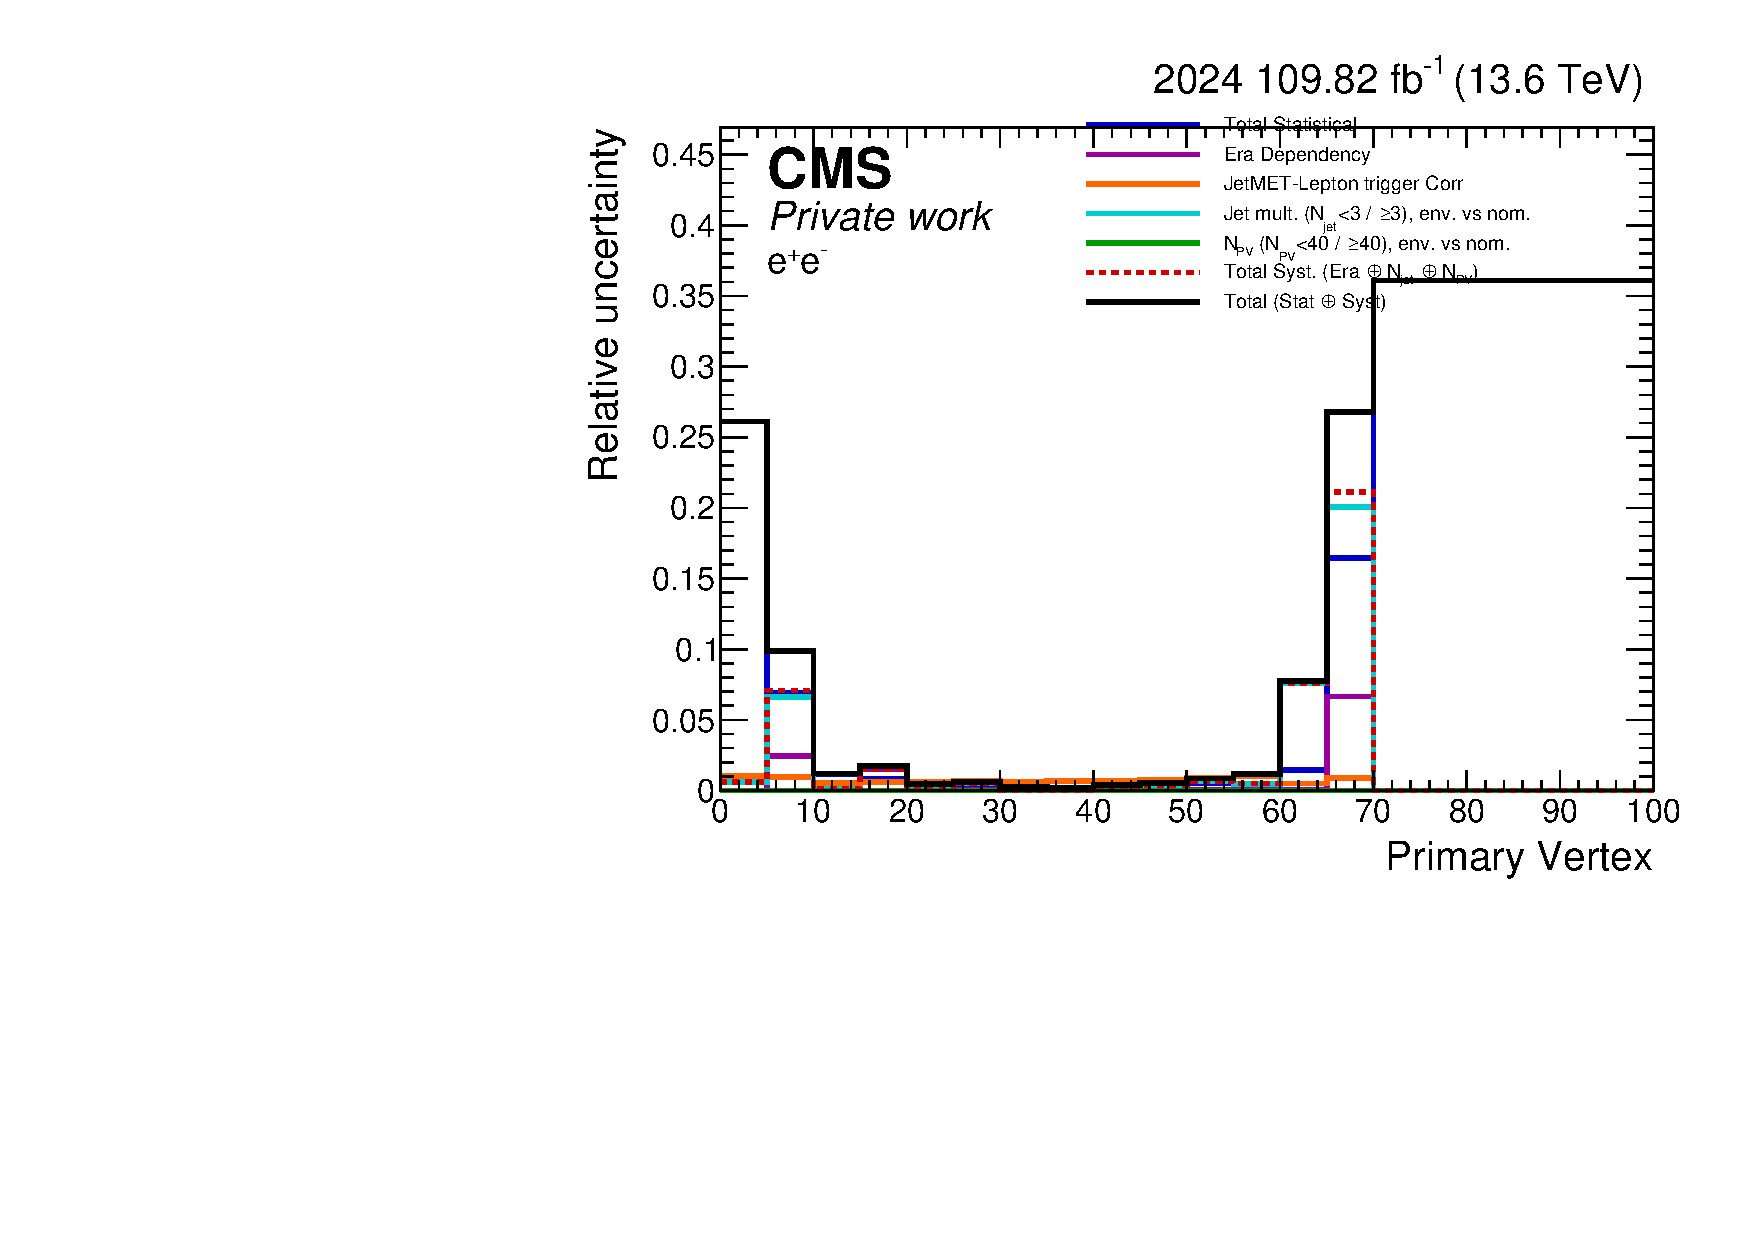
\includegraphics[width=0.48\linewidth]{figures/2024/ElEl/Relative_Uncertainty_Breakdown/Breakdown_Num_PV.pdf}
\caption{Relative uncertainty component breakdown versus event activity in the $ee$ channel. Left and right: jet and primary-vertex multiplicities.}\label{fig:extra-ElEl-Relative-Uncertainty-Breakdown-Num_Jets}\end{figure}
\begin{figure}[p]\centering
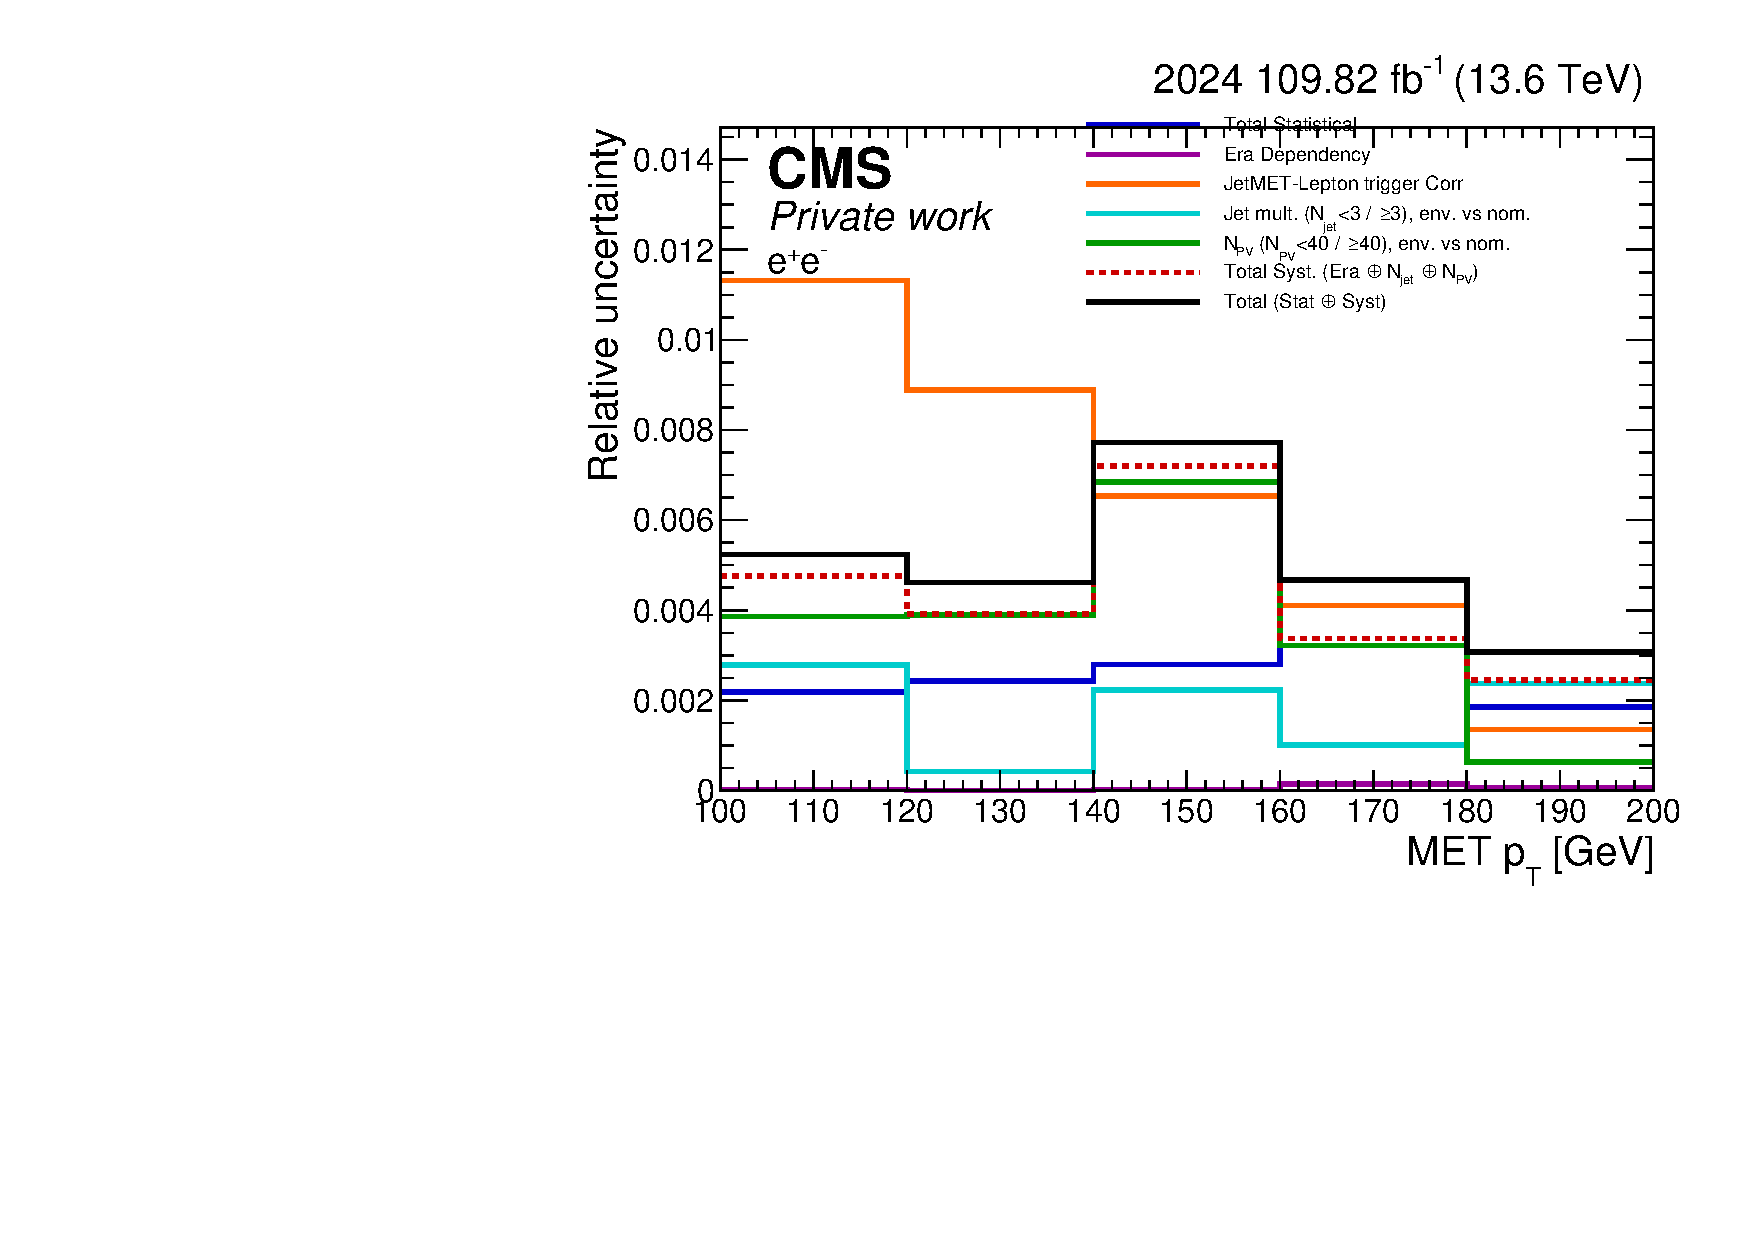
\includegraphics[width=0.48\linewidth]{figures/2024/ElEl/Relative_Uncertainty_Breakdown/Breakdown_METpt.pdf}
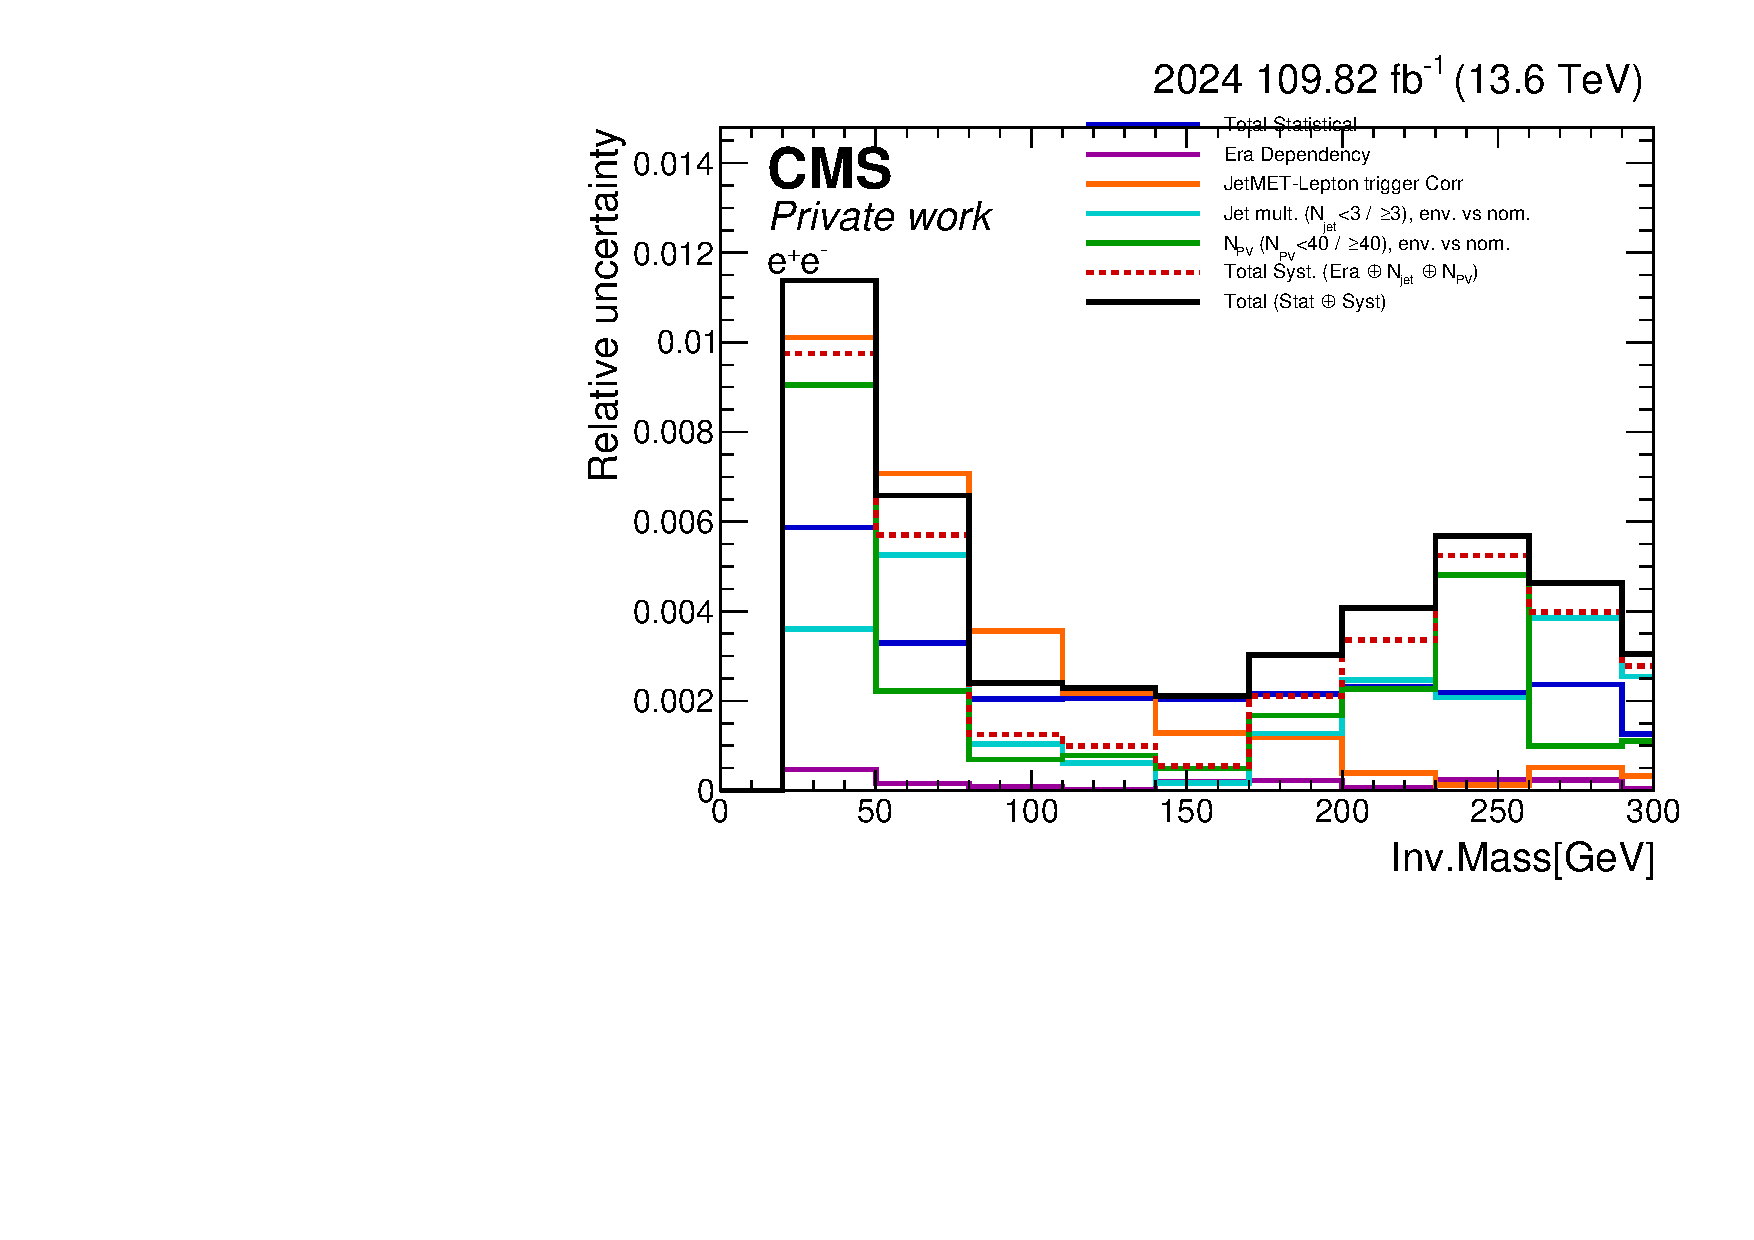
\includegraphics[width=0.48\linewidth]{figures/2024/ElEl/Relative_Uncertainty_Breakdown/Breakdown_DiLepMass.pdf}
\caption{Relative uncertainty component breakdown versus event kinematics in the $ee$ channel. Left and right: missing transverse momentum and dilepton invariant mass.}\label{fig:extra-ElEl-Relative-Uncertainty-Breakdown-METpt}\end{figure}
\begin{figure}[p]\centering
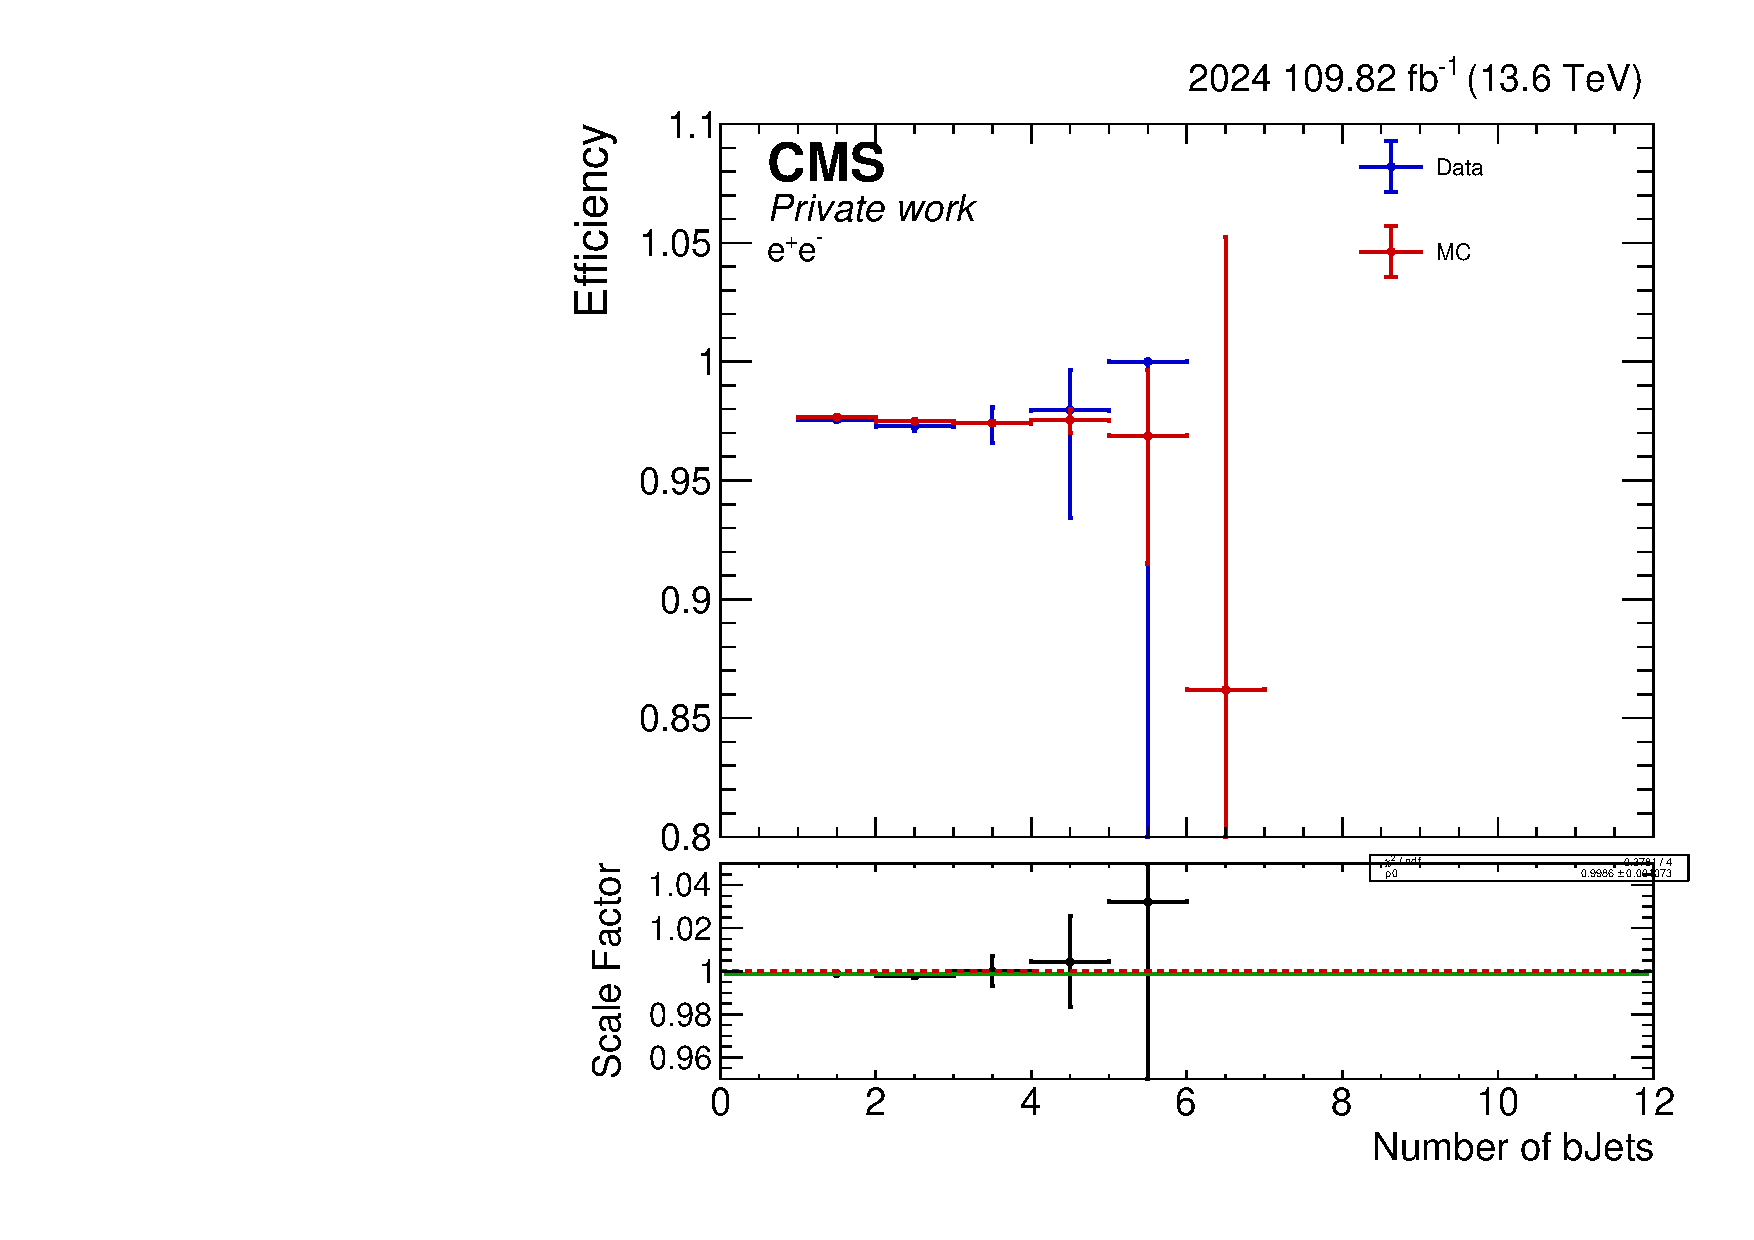
\includegraphics[width=0.48\linewidth]{figures/2024/ElEl/ScaleFactor/SF_Num_bJets.pdf}
\caption{Efficiency comparison and scale factor versus heavy-flavour activity in the $ee$ channel. $b$-tagged jet multiplicity.}\label{fig:extra-ElEl-ScaleFactor-Num_bJets}\end{figure}
\clearpage\subsection{$e\mu$ channel}
\begin{figure}[p]\centering
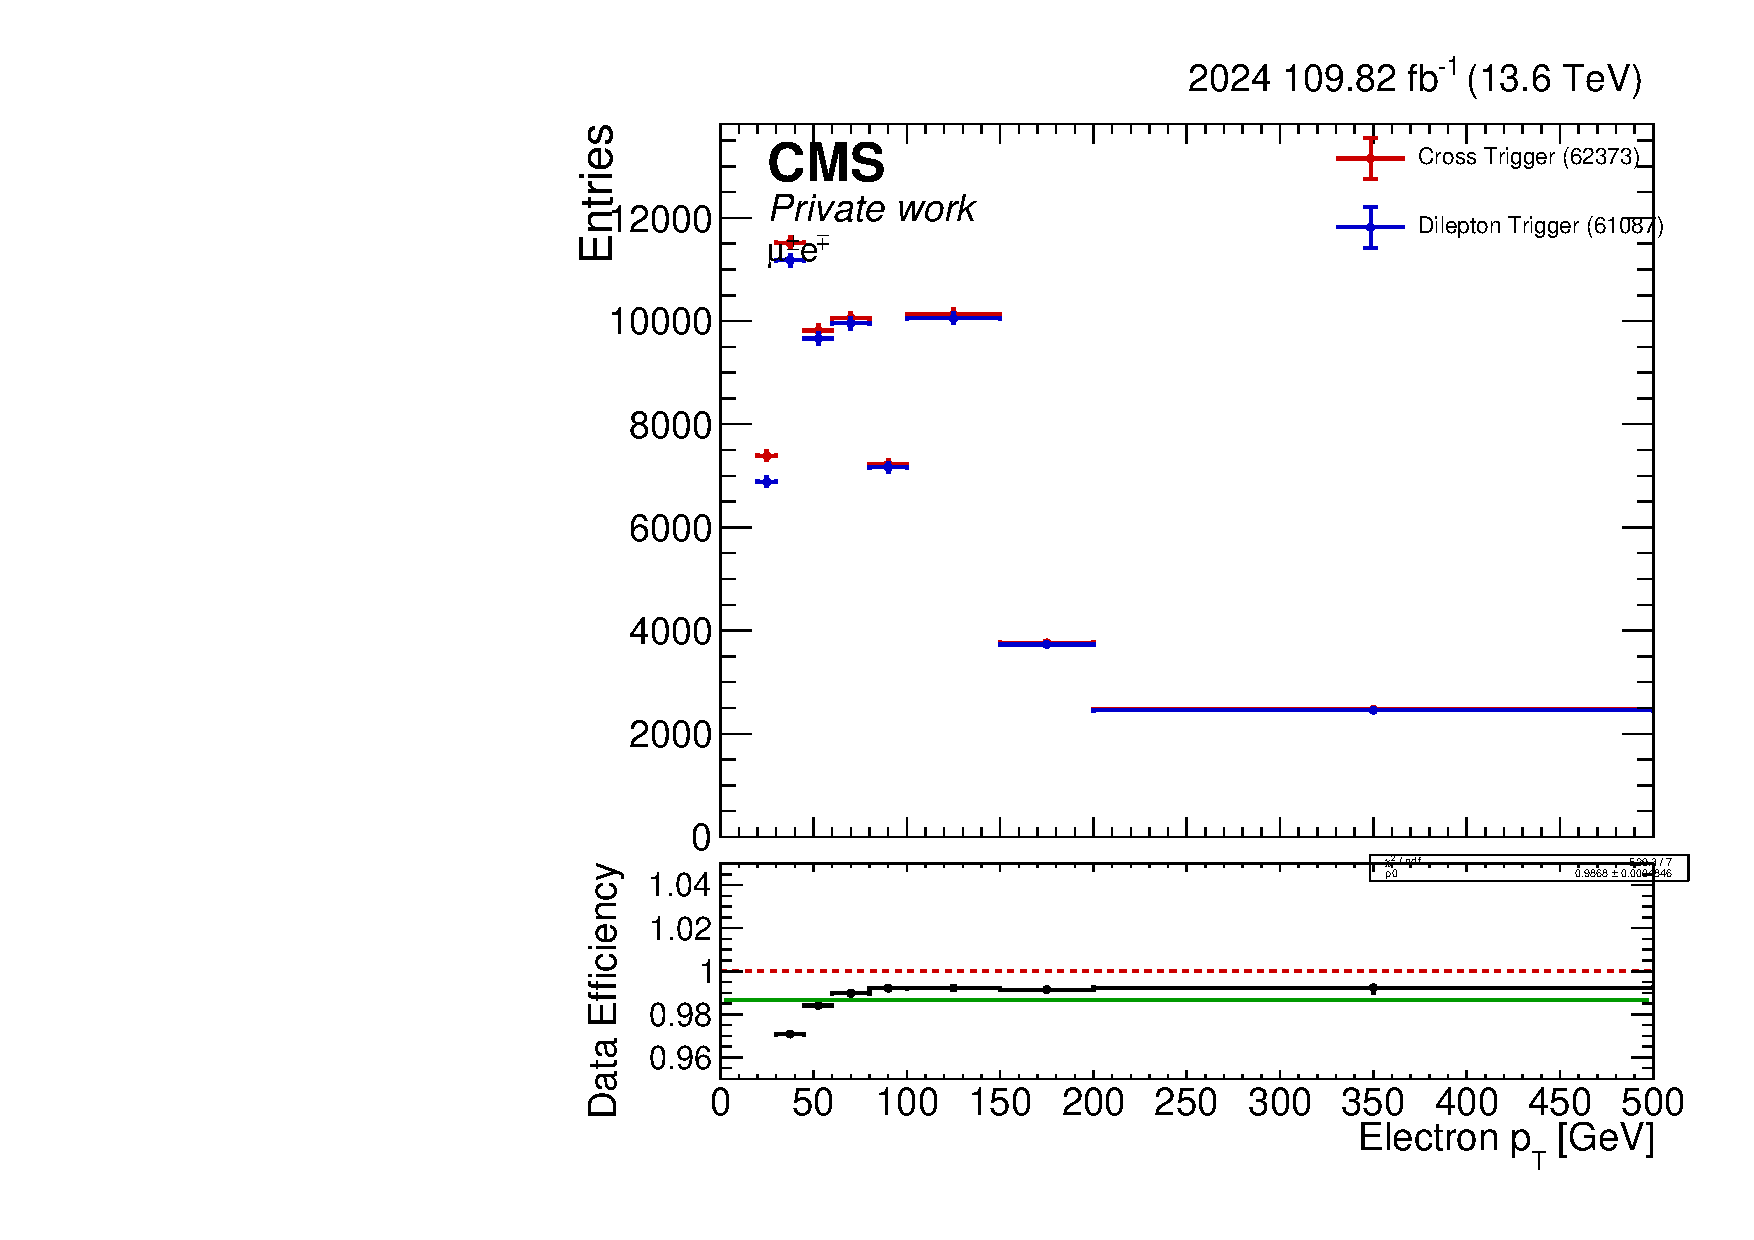
\includegraphics[width=0.48\linewidth]{figures/2024/MuEl/TrigEffData/TrigEff_ElPt.pdf}
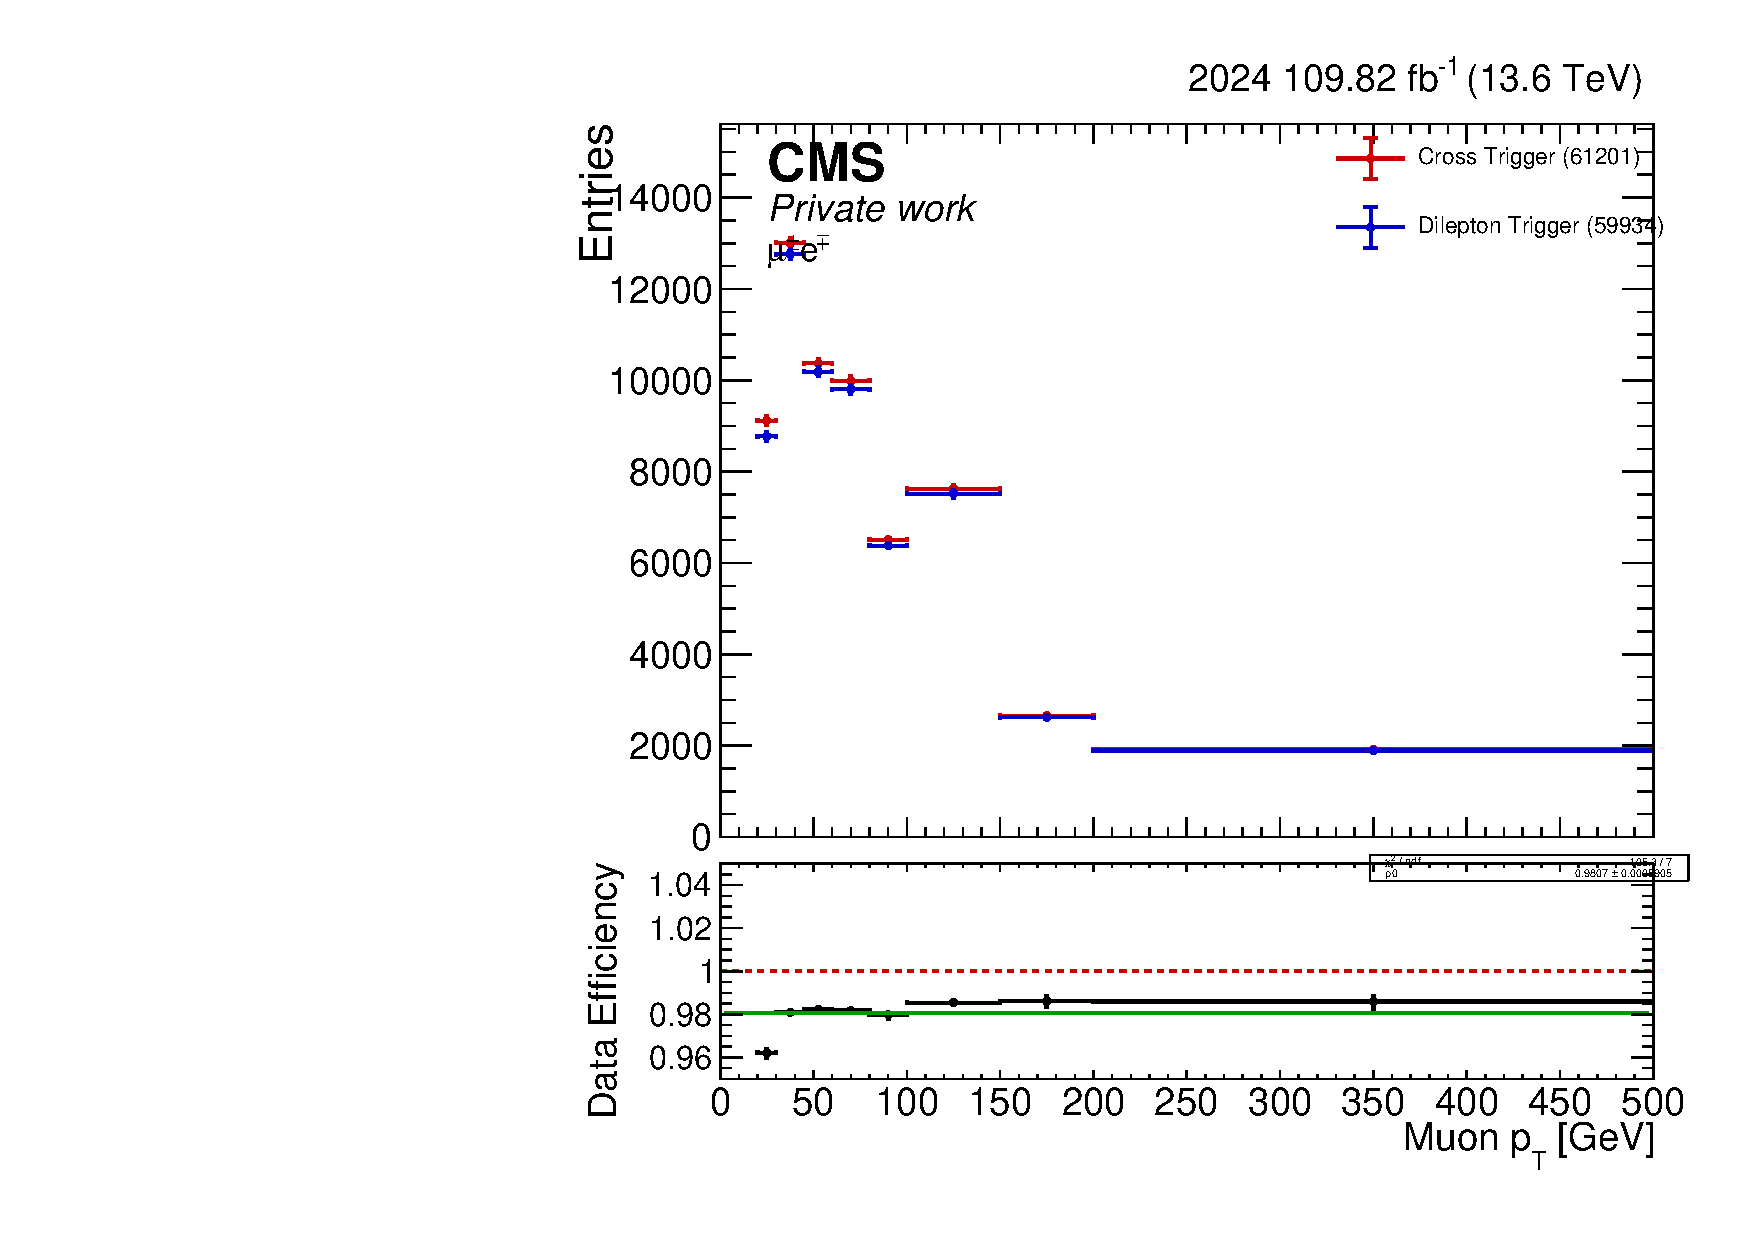
\includegraphics[width=0.48\linewidth]{figures/2024/MuEl/TrigEffData/TrigEff_MuPt.pdf}
\caption{Data trigger numerator and reference-sample distributions (upper panels), with their efficiency ratios (lower panels) in the $e\mu$ channel. Left and right: electron and muon $p_{\mathrm{T}}$.}\label{fig:extra-MuEl-TrigEffData-ElPt}\end{figure}
\begin{figure}[p]\centering
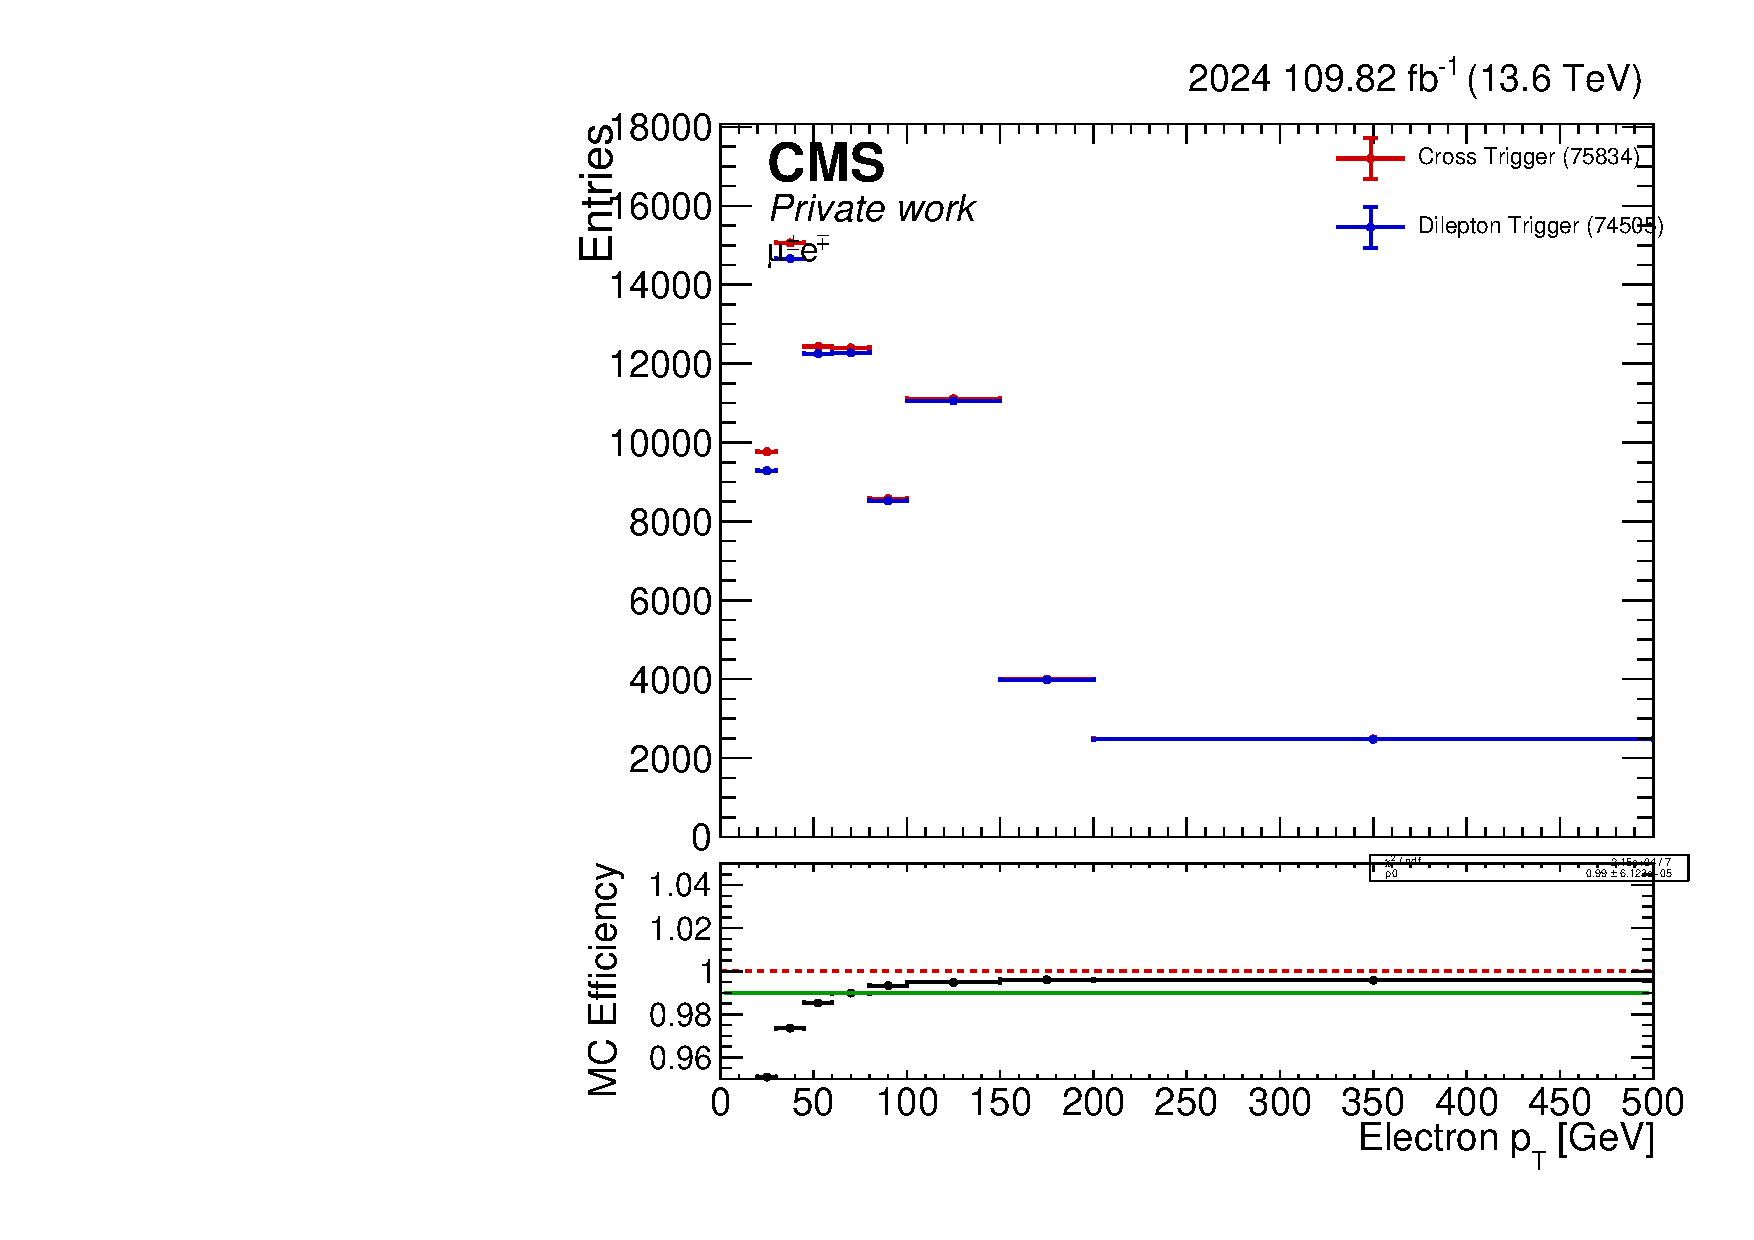
\includegraphics[width=0.48\linewidth]{figures/2024/MuEl/TrigEffMC/TrigEff_ElPt.pdf}
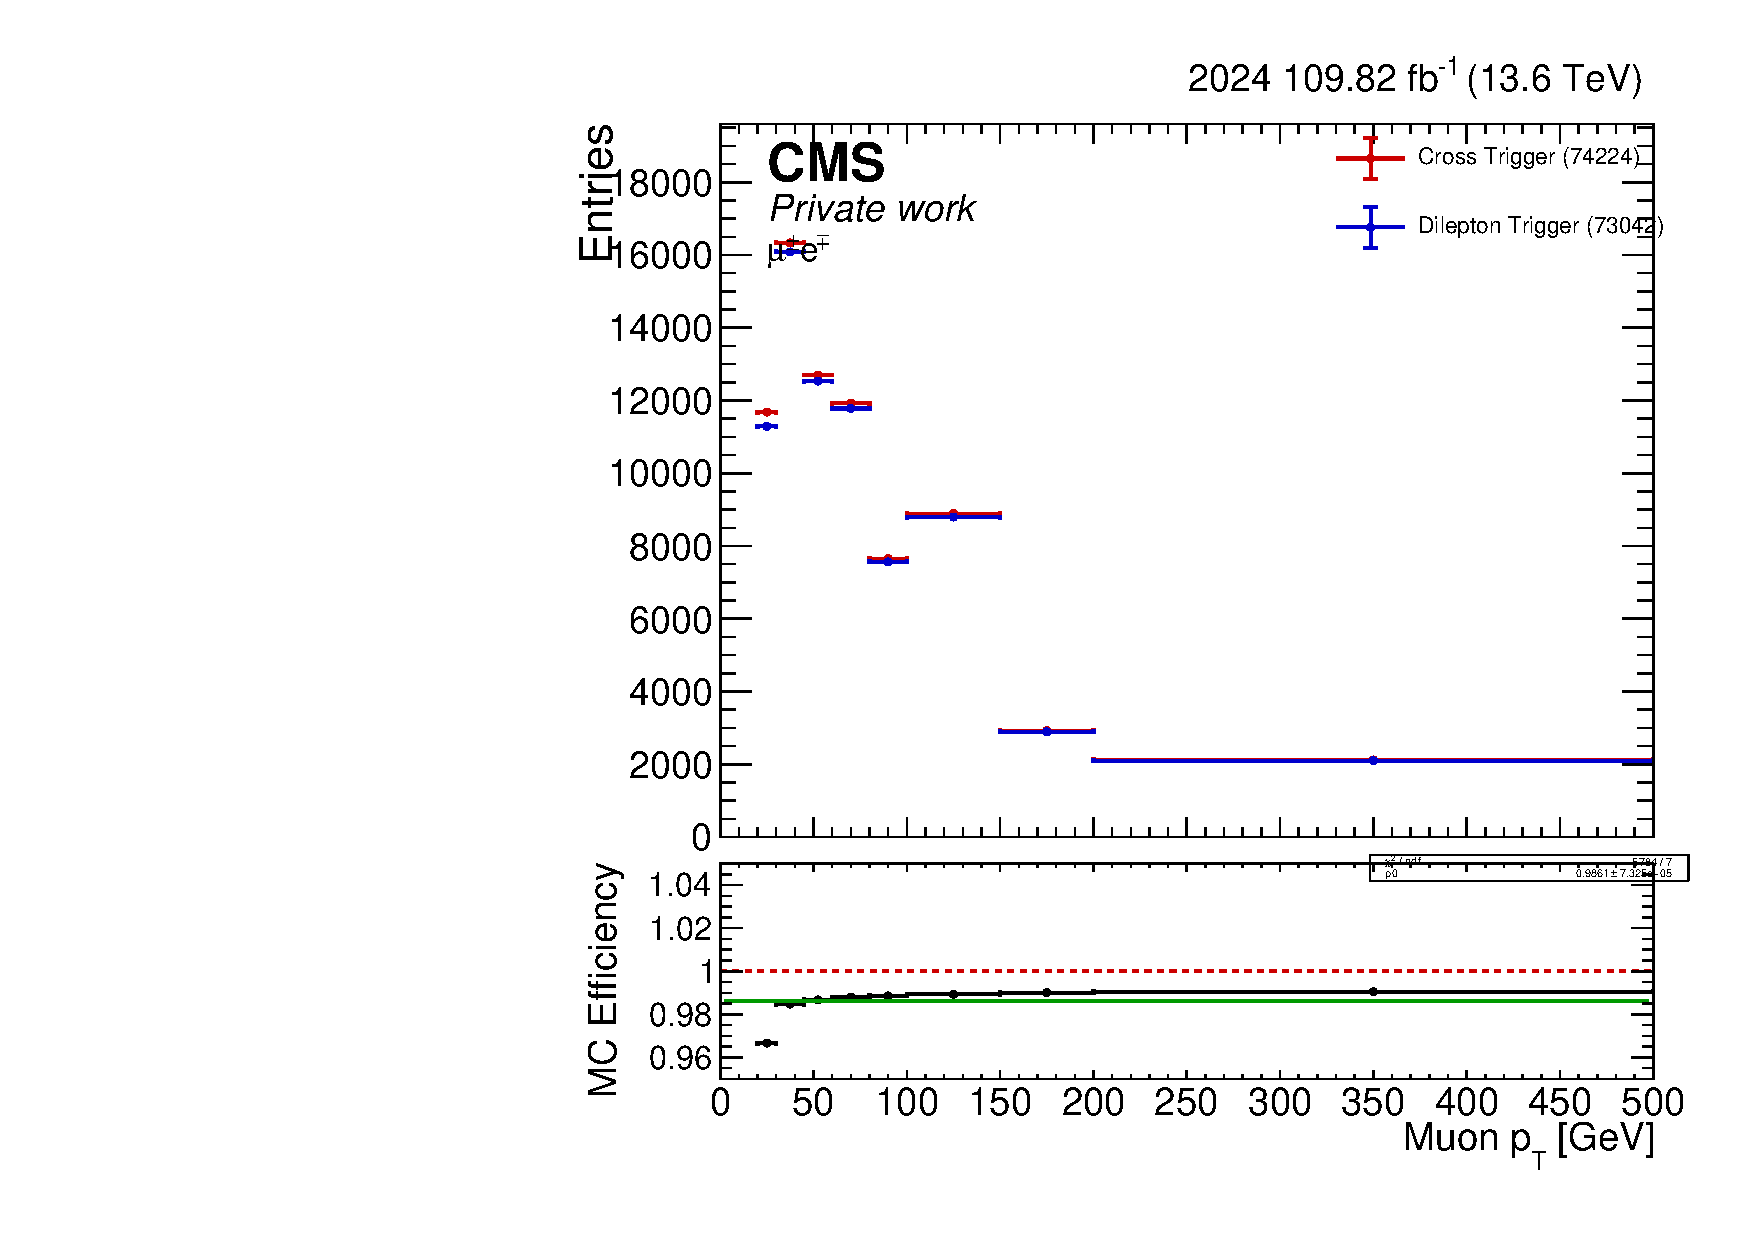
\includegraphics[width=0.48\linewidth]{figures/2024/MuEl/TrigEffMC/TrigEff_MuPt.pdf}
\caption{Simulated trigger numerator and reference-sample distributions (upper panels), with their efficiency ratios (lower panels) in the $e\mu$ channel. Left and right: electron and muon $p_{\mathrm{T}}$.}\label{fig:extra-MuEl-TrigEffMC-ElPt}\end{figure}
\begin{figure}[p]\centering
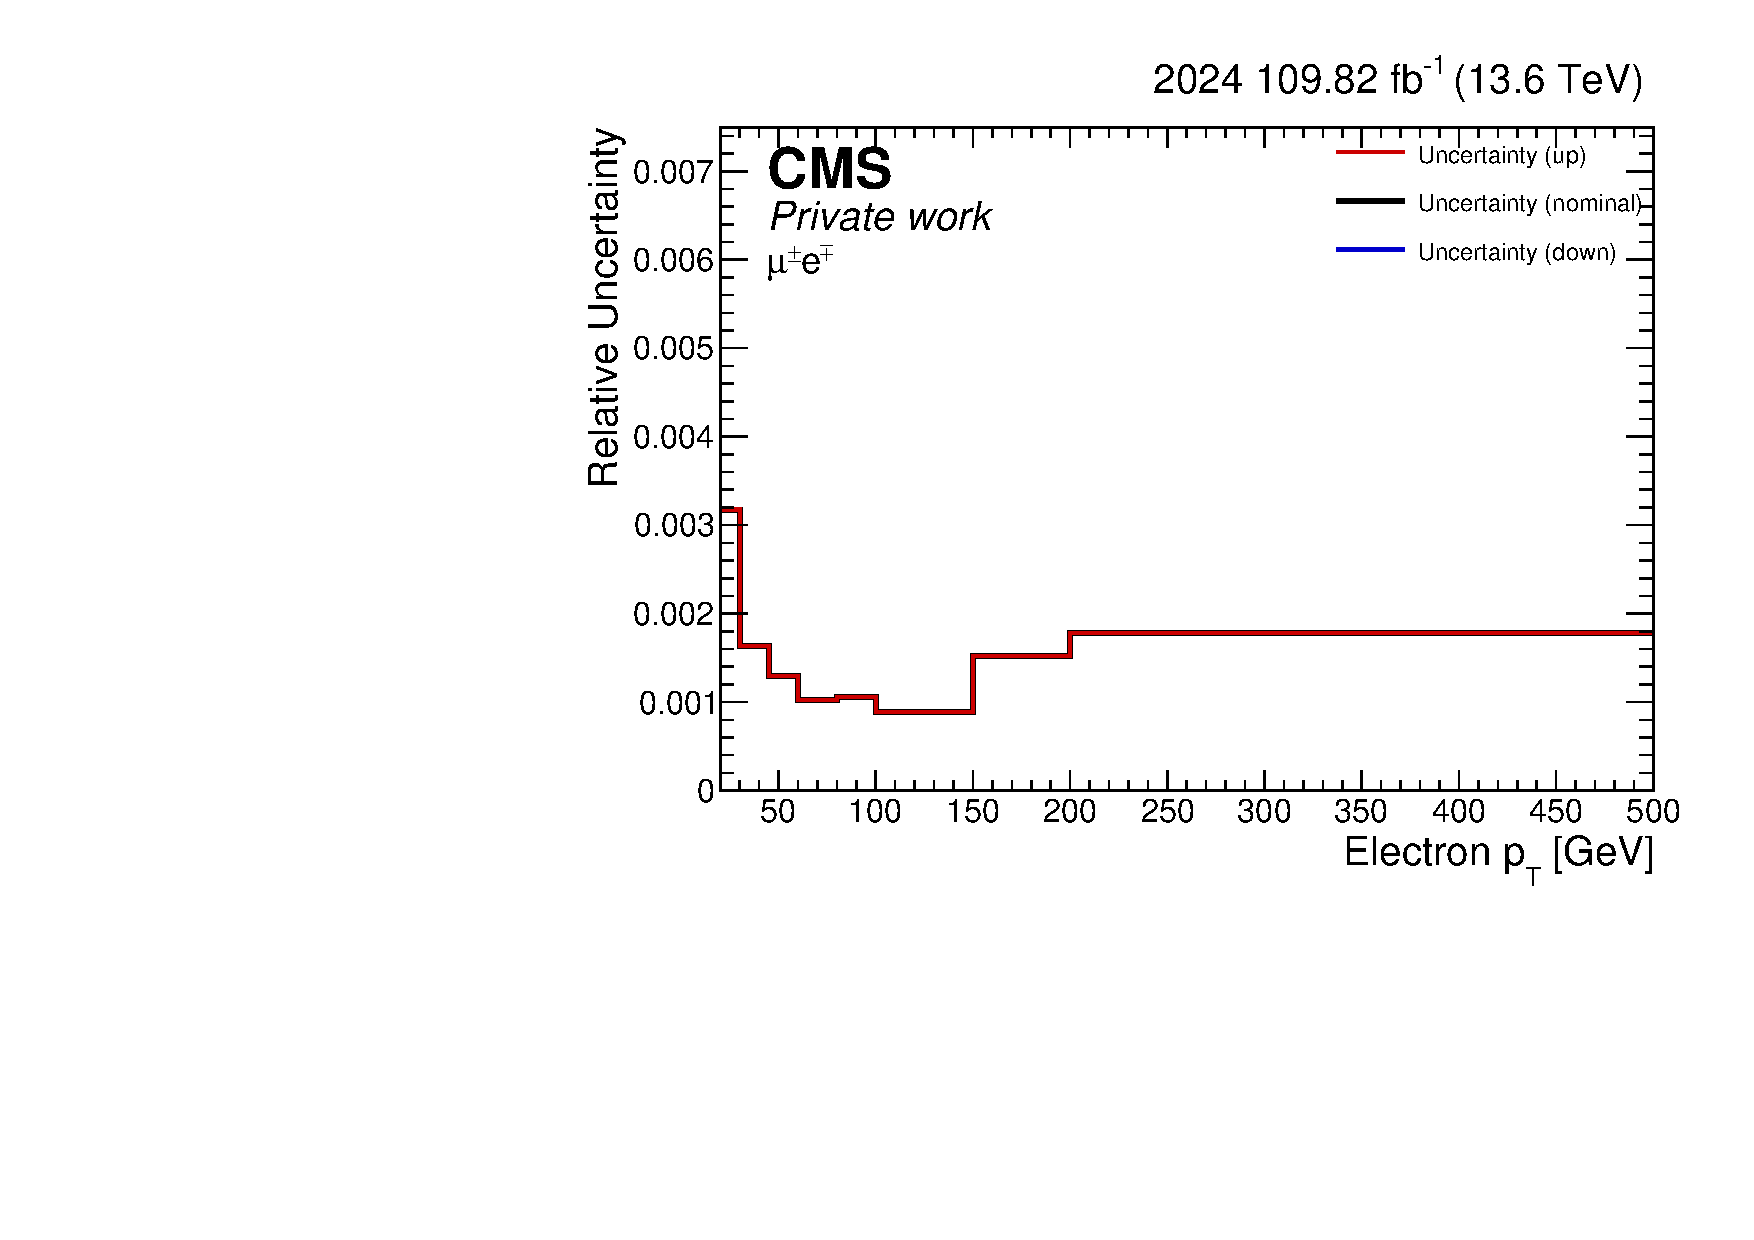
\includegraphics[width=0.48\linewidth]{figures/2024/MuEl/Statistical_Uncertainty/UncRatio_ElPt.pdf}
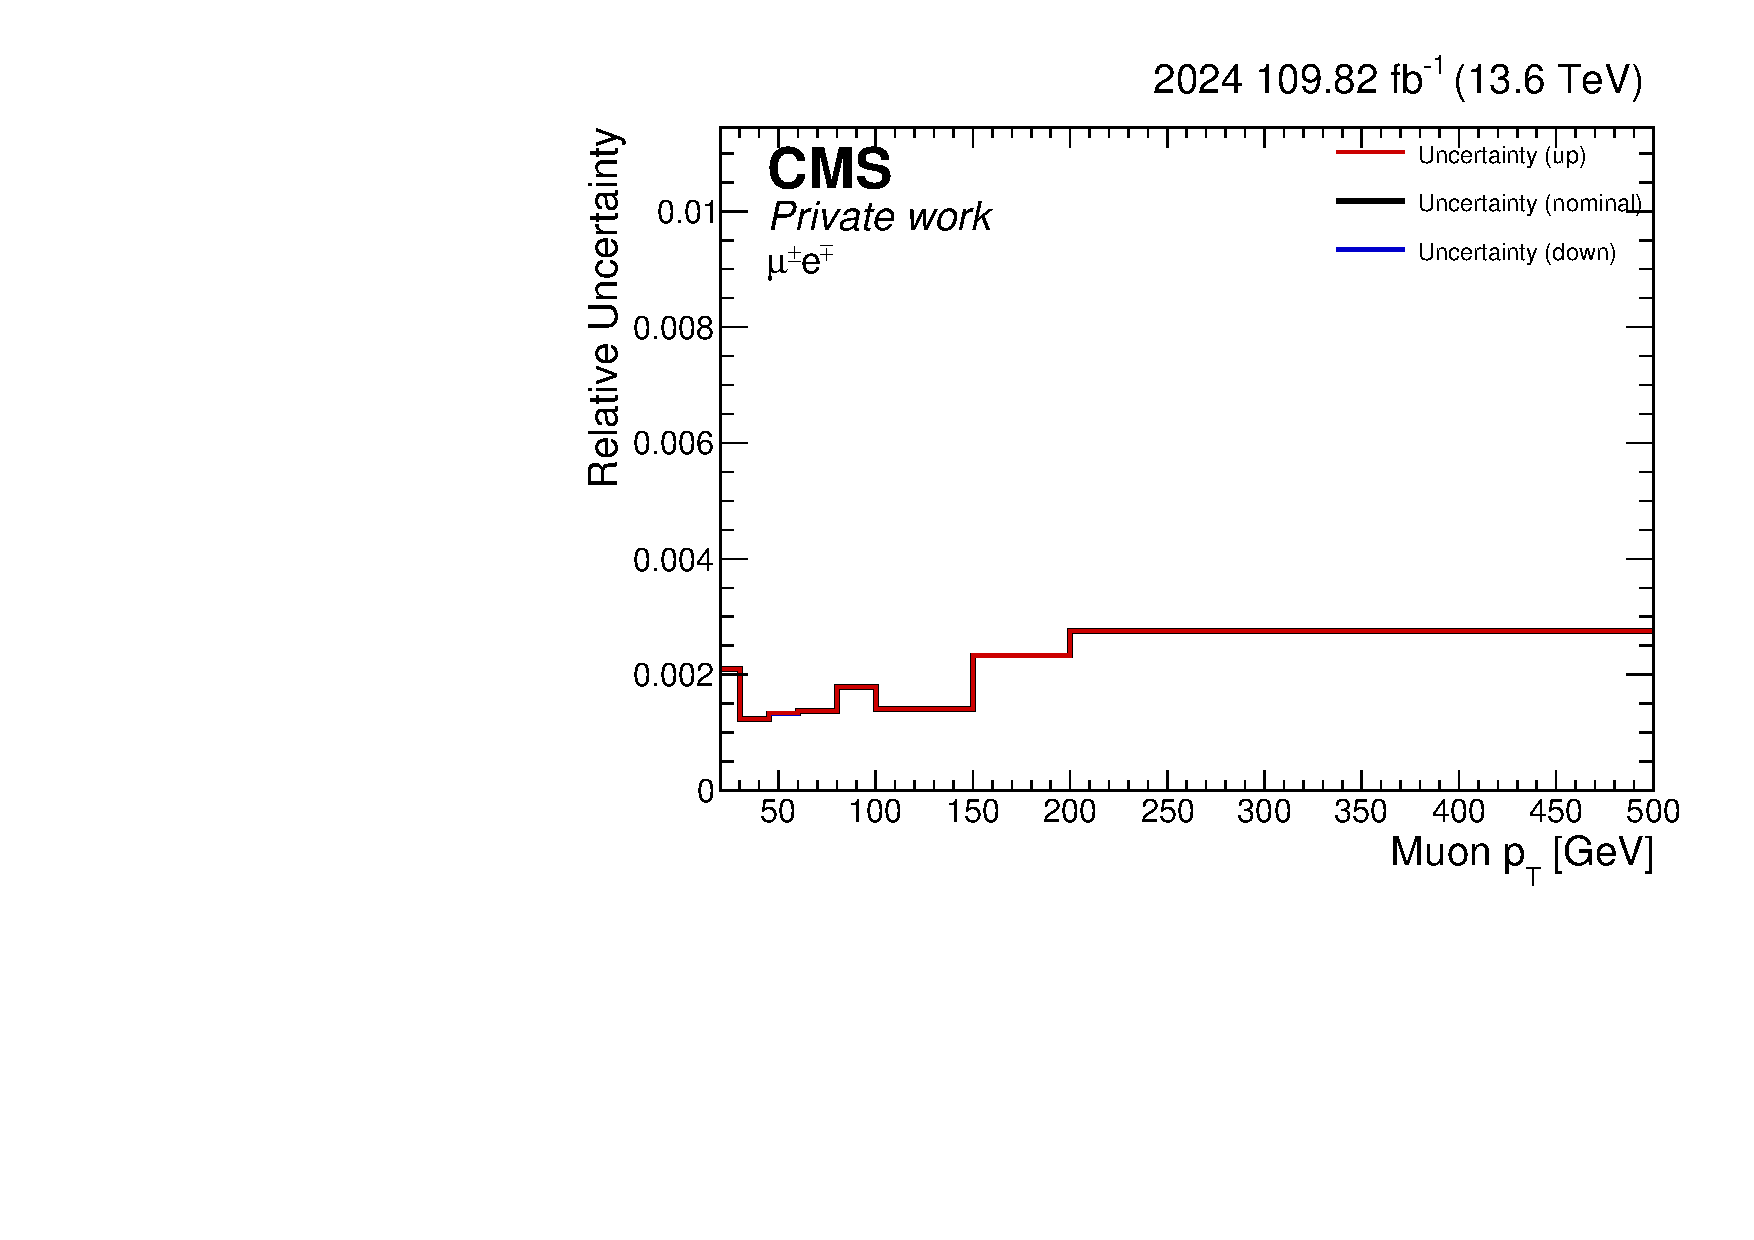
\includegraphics[width=0.48\linewidth]{figures/2024/MuEl/Statistical_Uncertainty/UncRatio_MuPt.pdf}
\caption{Relative statistical uncertainty diagnostics, retaining the nominal, upward, and downward curves of the supplied production in the $e\mu$ channel. Left and right: electron and muon $p_{\mathrm{T}}$.}\label{fig:extra-MuEl-Statistical-Uncertainty-ElPt}\end{figure}
\begin{figure}[p]\centering
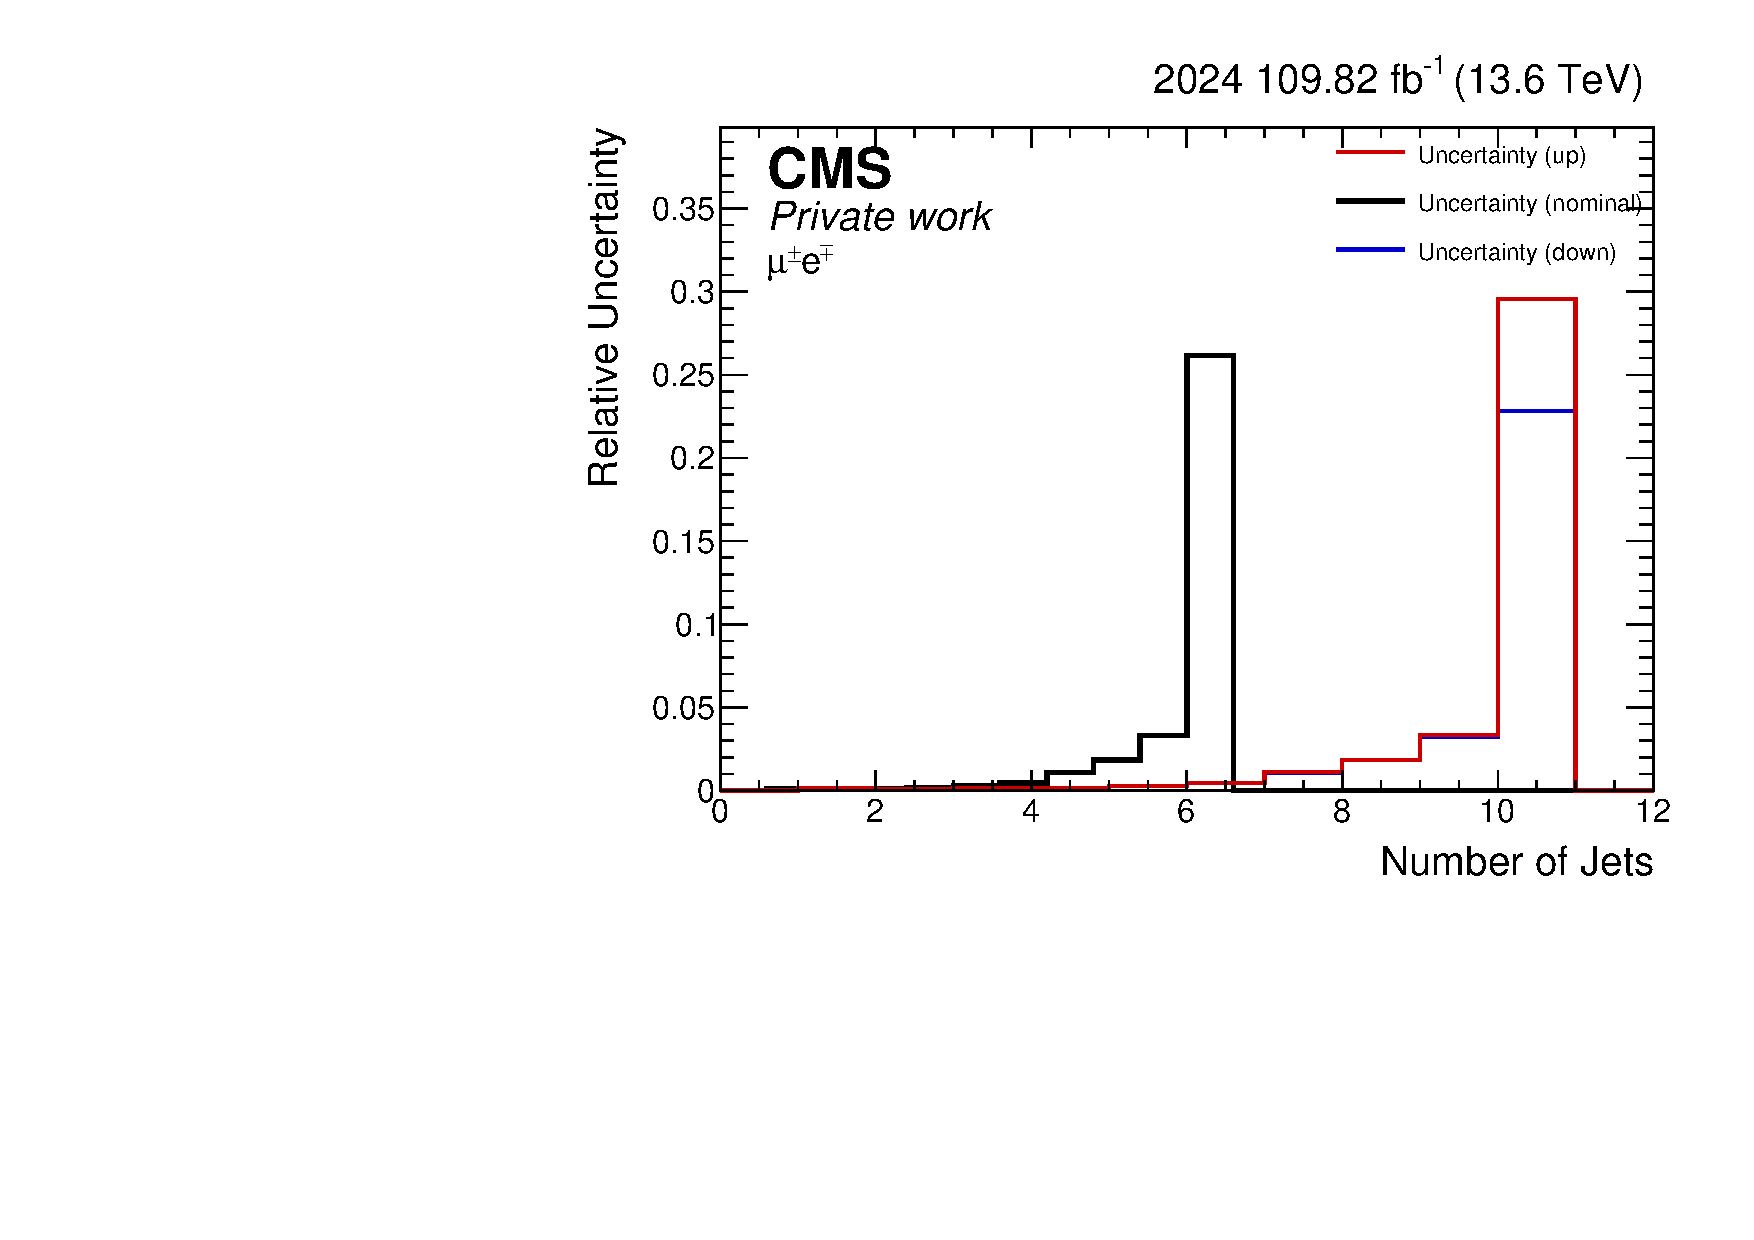
\includegraphics[width=0.48\linewidth]{figures/2024/MuEl/Statistical_Uncertainty/UncRatio_Num_Jets.pdf}
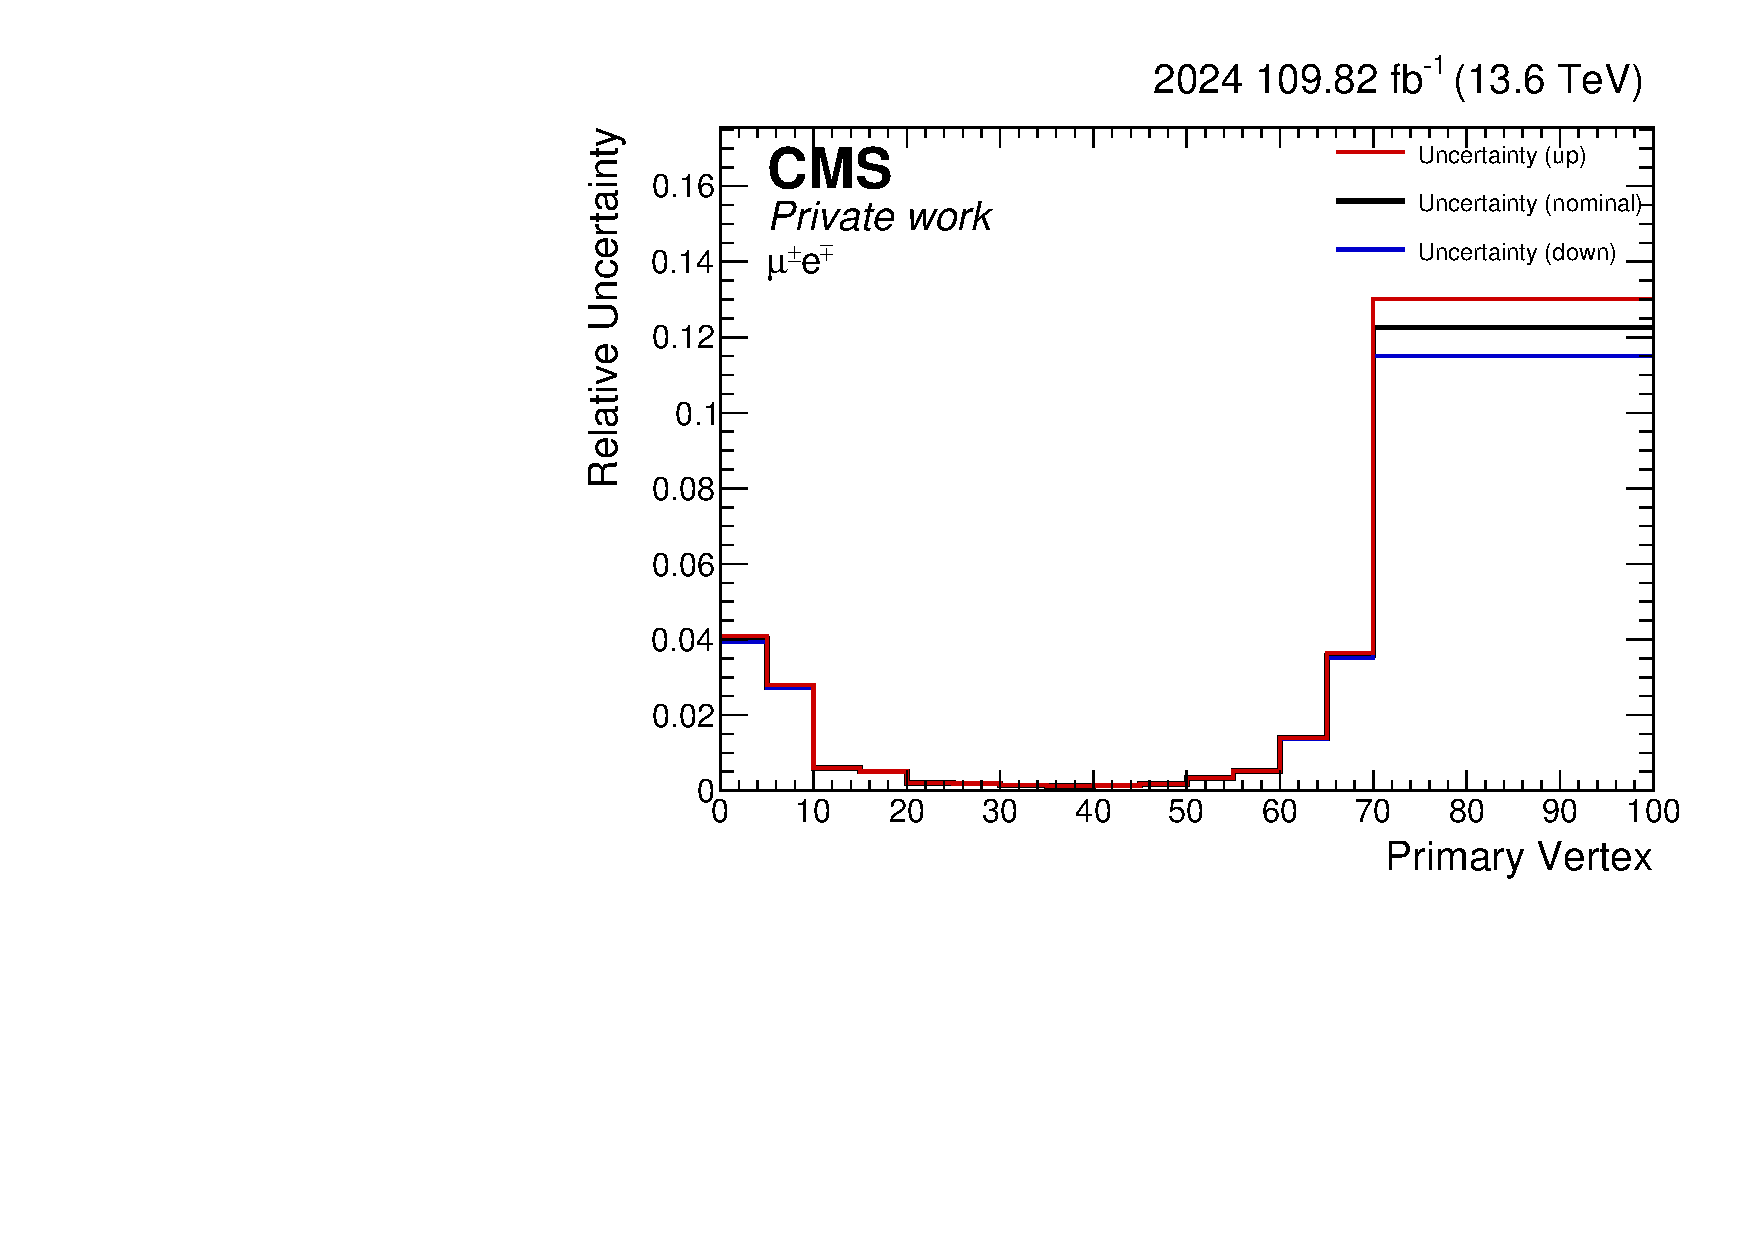
\includegraphics[width=0.48\linewidth]{figures/2024/MuEl/Statistical_Uncertainty/UncRatio_Num_PV.pdf}
\caption{Relative statistical uncertainty diagnostics, retaining the nominal, upward, and downward curves of the supplied production in the $e\mu$ channel. Left and right: jet and primary-vertex multiplicities.}\label{fig:extra-MuEl-Statistical-Uncertainty-Num_Jets}\end{figure}
\begin{figure}[p]\centering
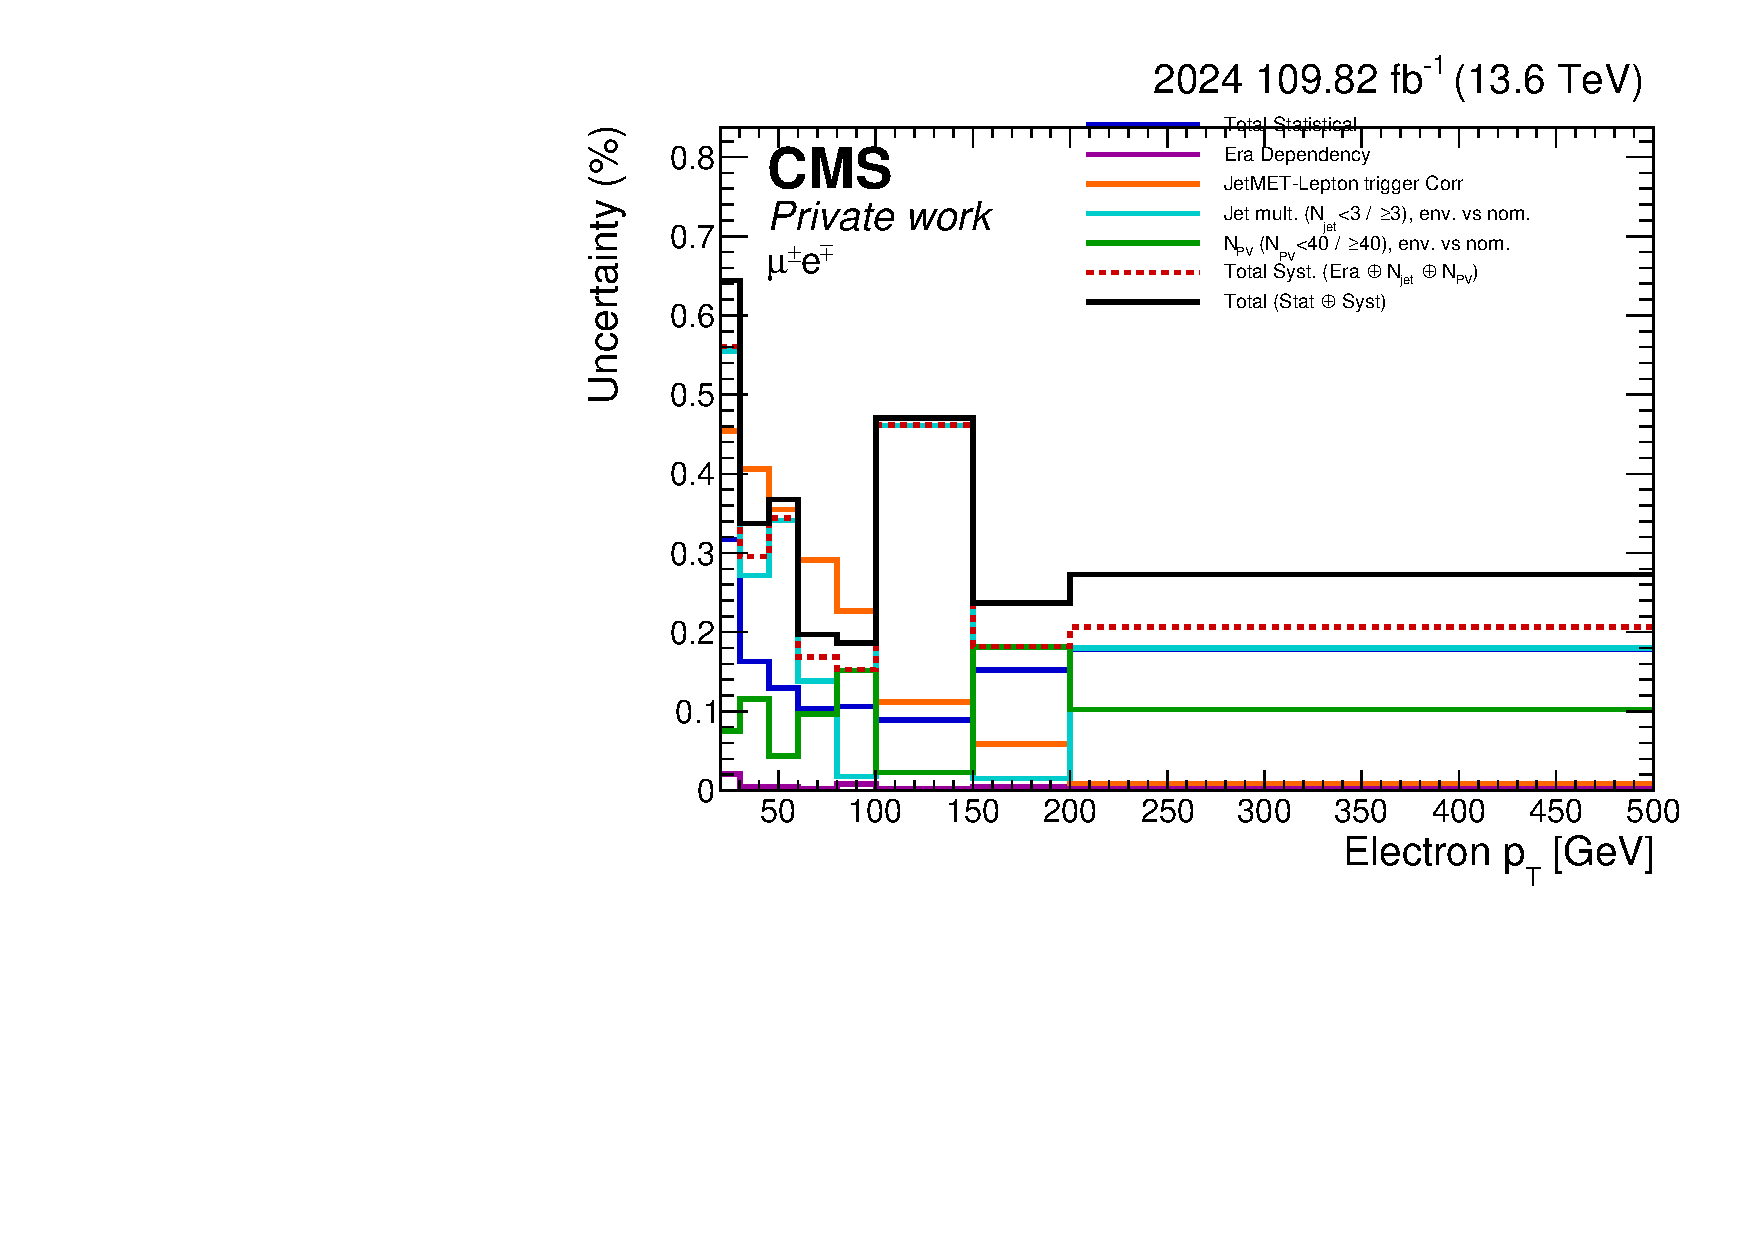
\includegraphics[width=0.48\linewidth]{figures/2024/MuEl/Uncertainty_Breakdown/Breakdown_ElPt.pdf}
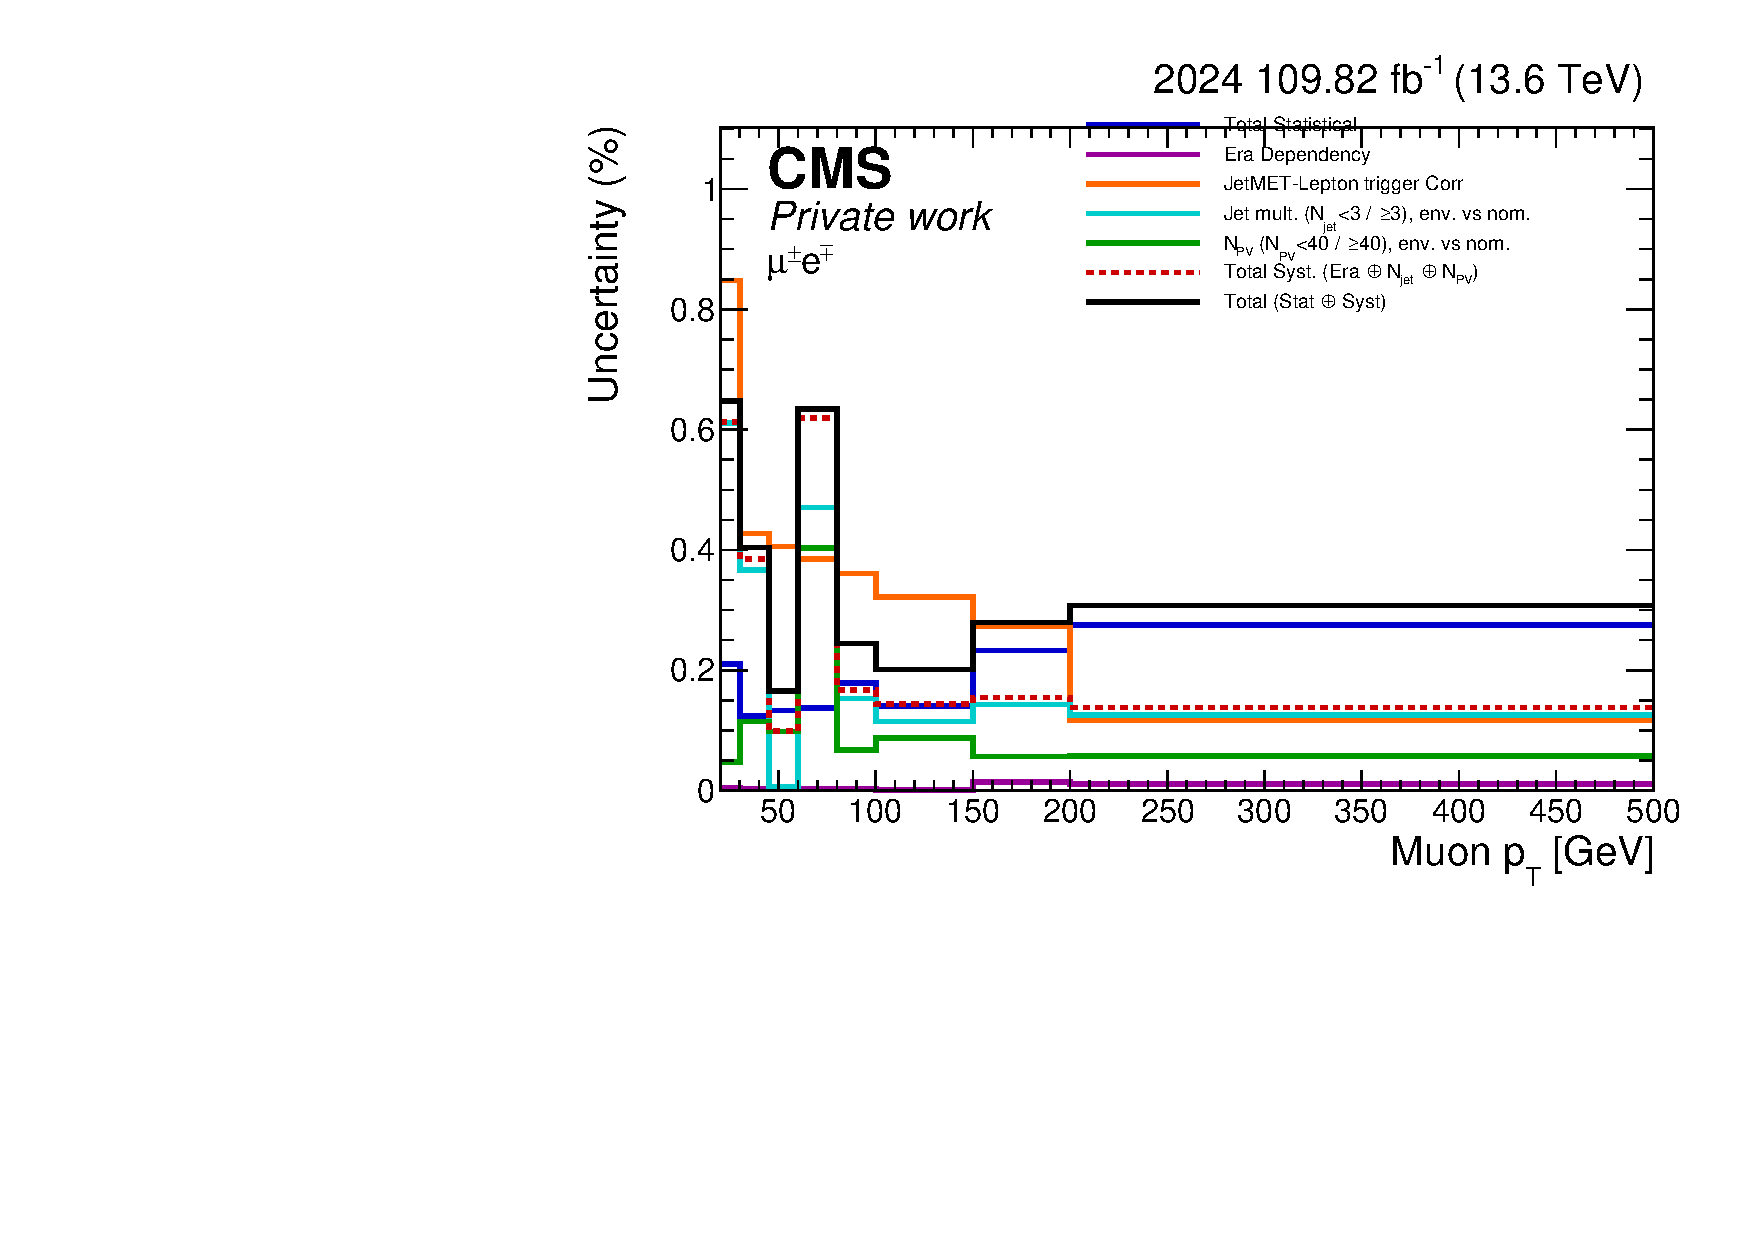
\includegraphics[width=0.48\linewidth]{figures/2024/MuEl/Uncertainty_Breakdown/Breakdown_MuPt.pdf}
\caption{Absolute uncertainty component breakdown in the $e\mu$ channel. Left and right: electron and muon $p_{\mathrm{T}}$.}\label{fig:extra-MuEl-Uncertainty-Breakdown-ElPt}\end{figure}
\begin{figure}[p]\centering
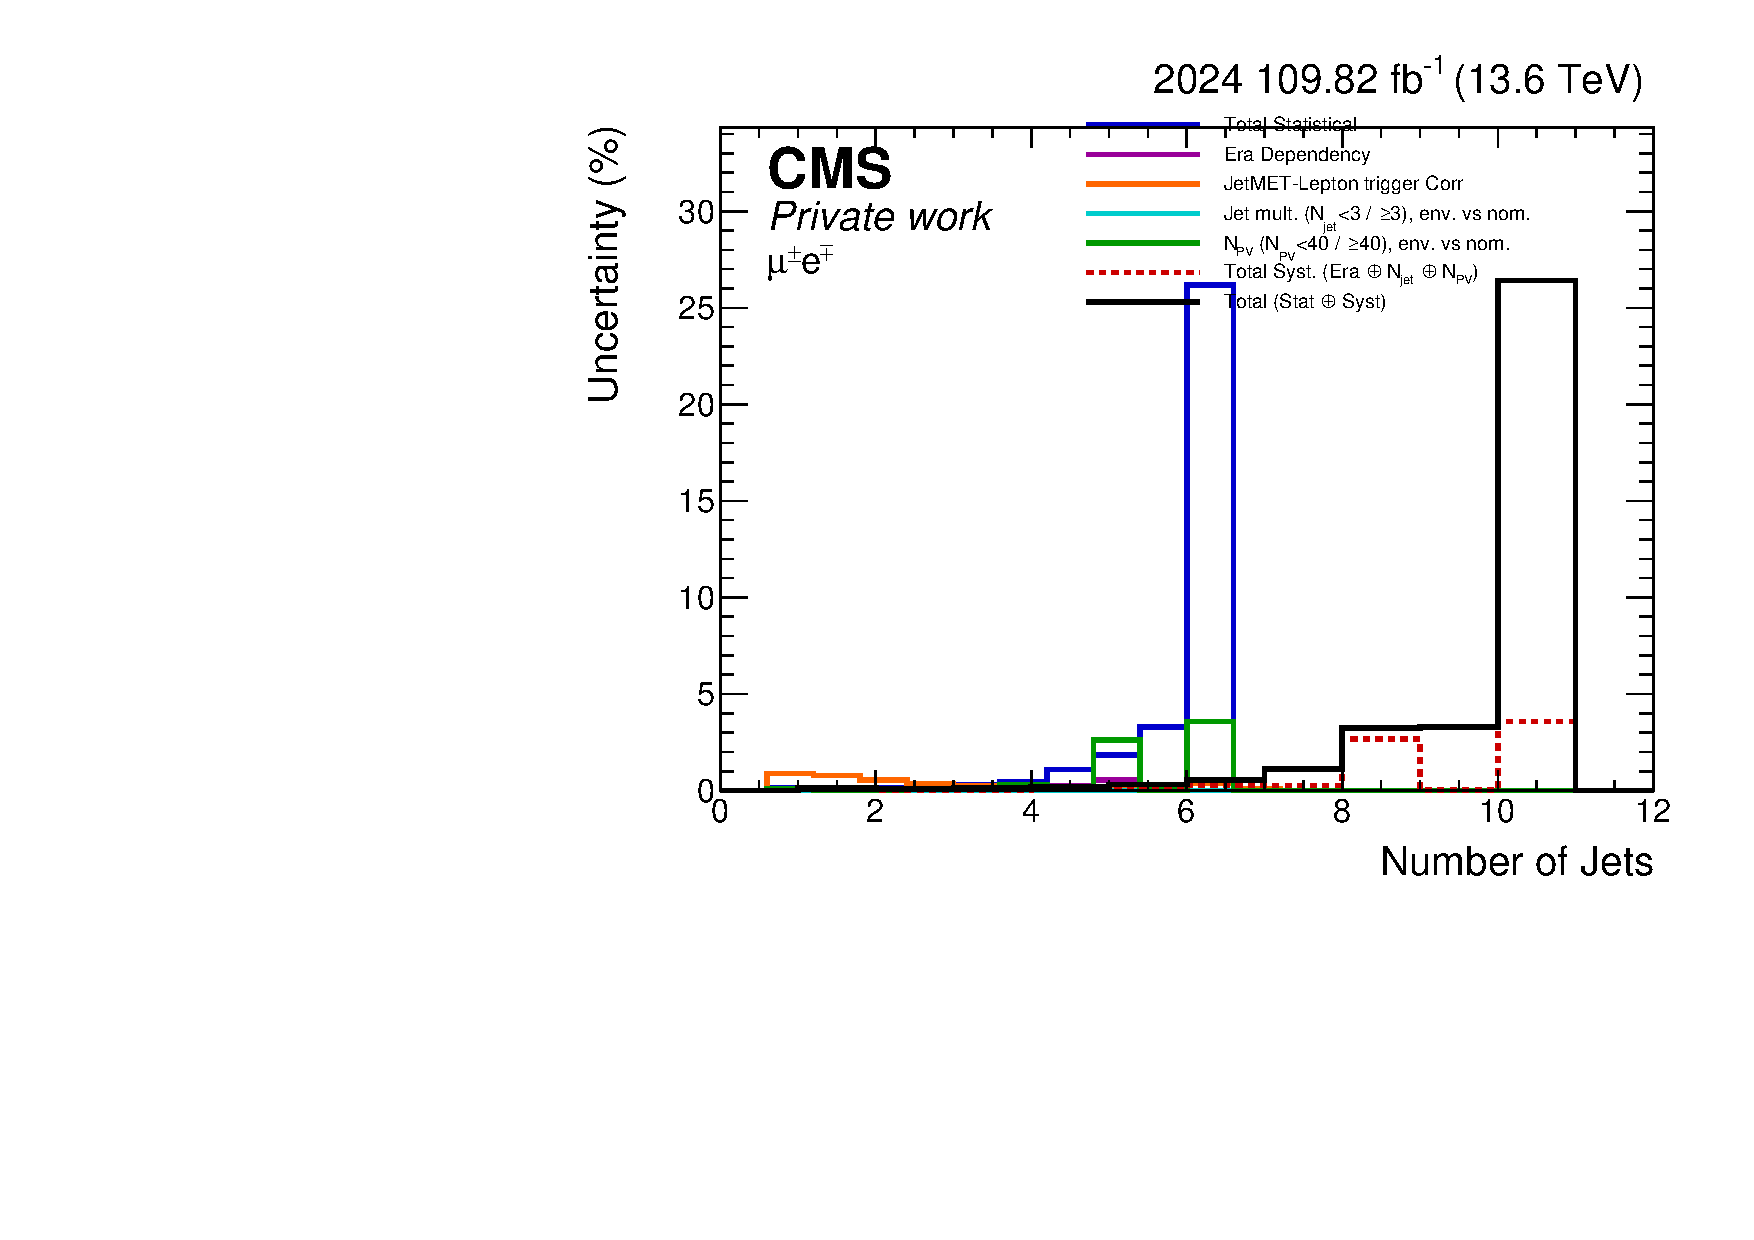
\includegraphics[width=0.48\linewidth]{figures/2024/MuEl/Uncertainty_Breakdown/Breakdown_Num_Jets.pdf}
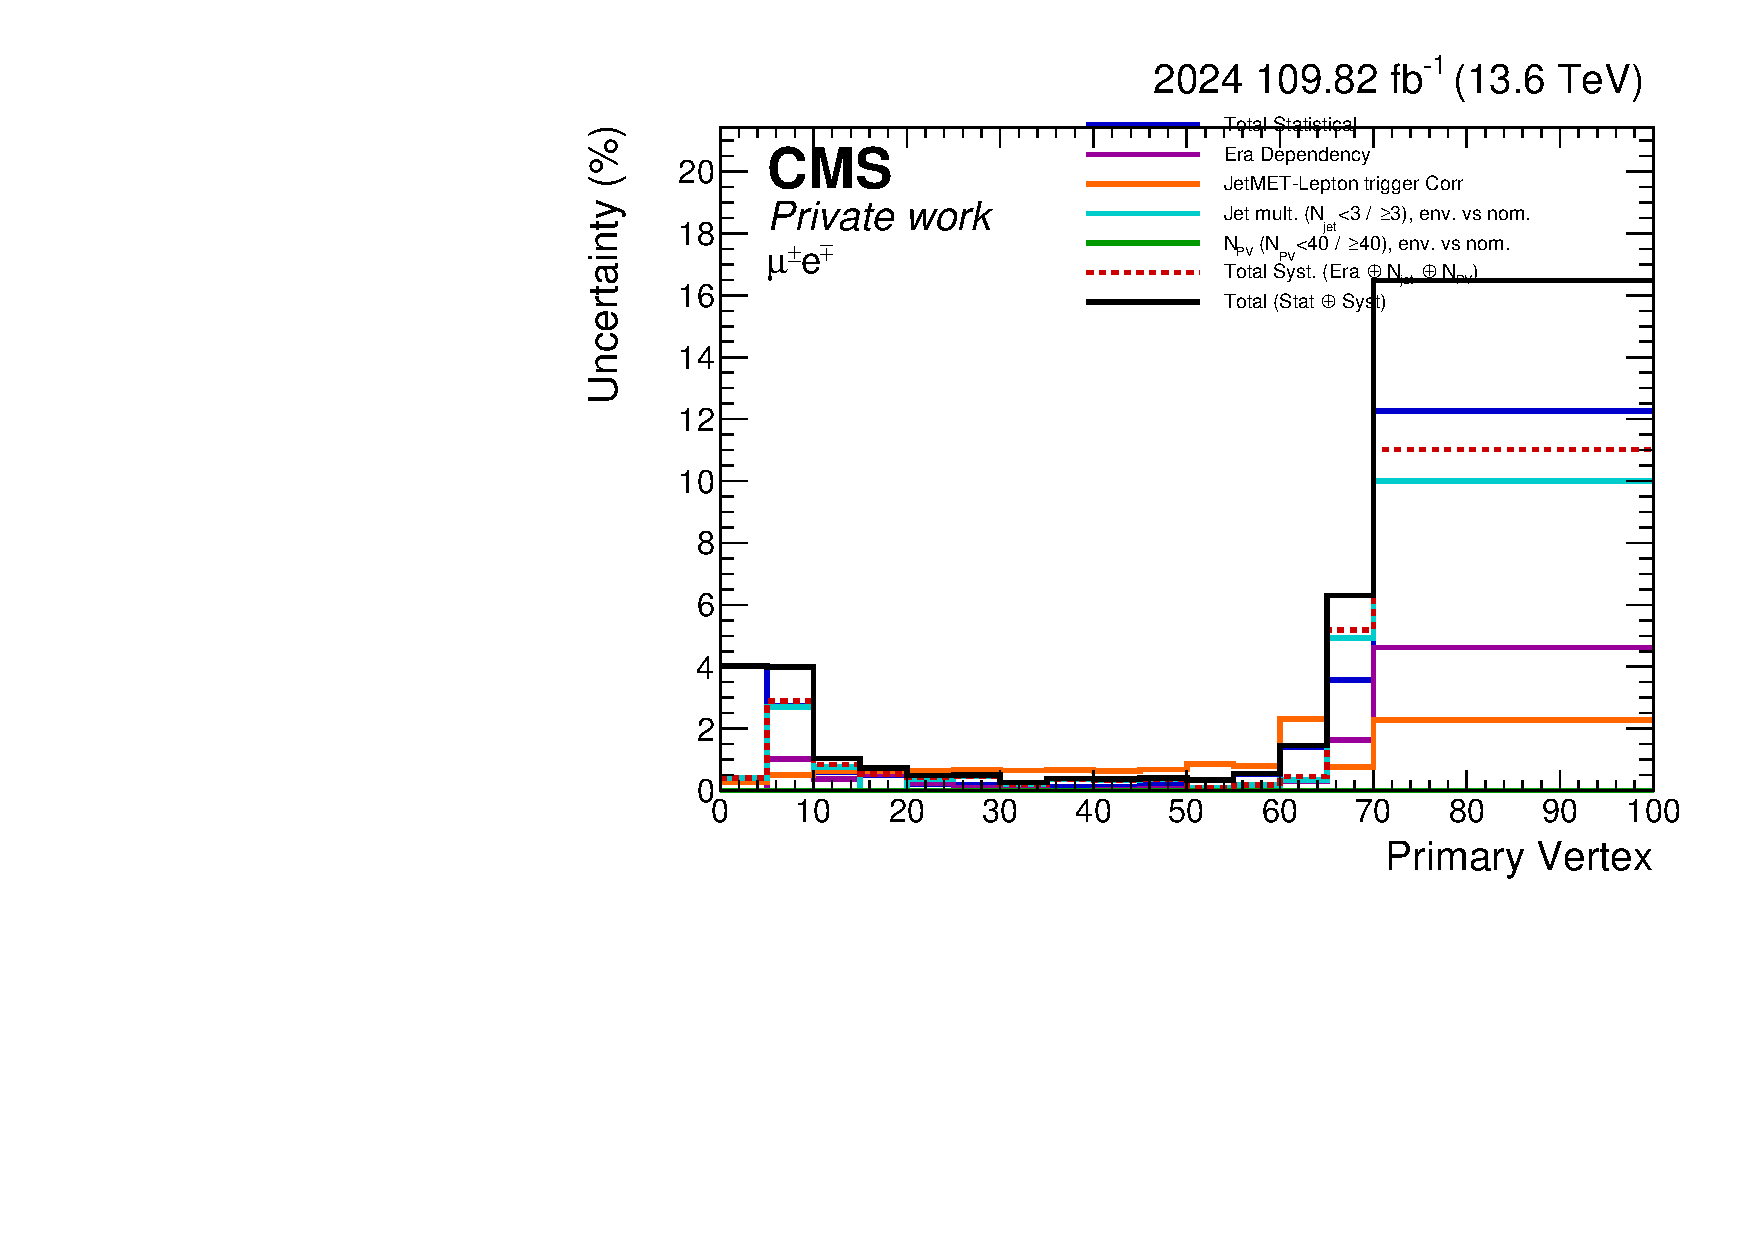
\includegraphics[width=0.48\linewidth]{figures/2024/MuEl/Uncertainty_Breakdown/Breakdown_Num_PV.pdf}
\caption{Absolute uncertainty component breakdown in the $e\mu$ channel. Left and right: jet and primary-vertex multiplicities.}\label{fig:extra-MuEl-Uncertainty-Breakdown-Num_Jets}\end{figure}
\begin{figure}[p]\centering
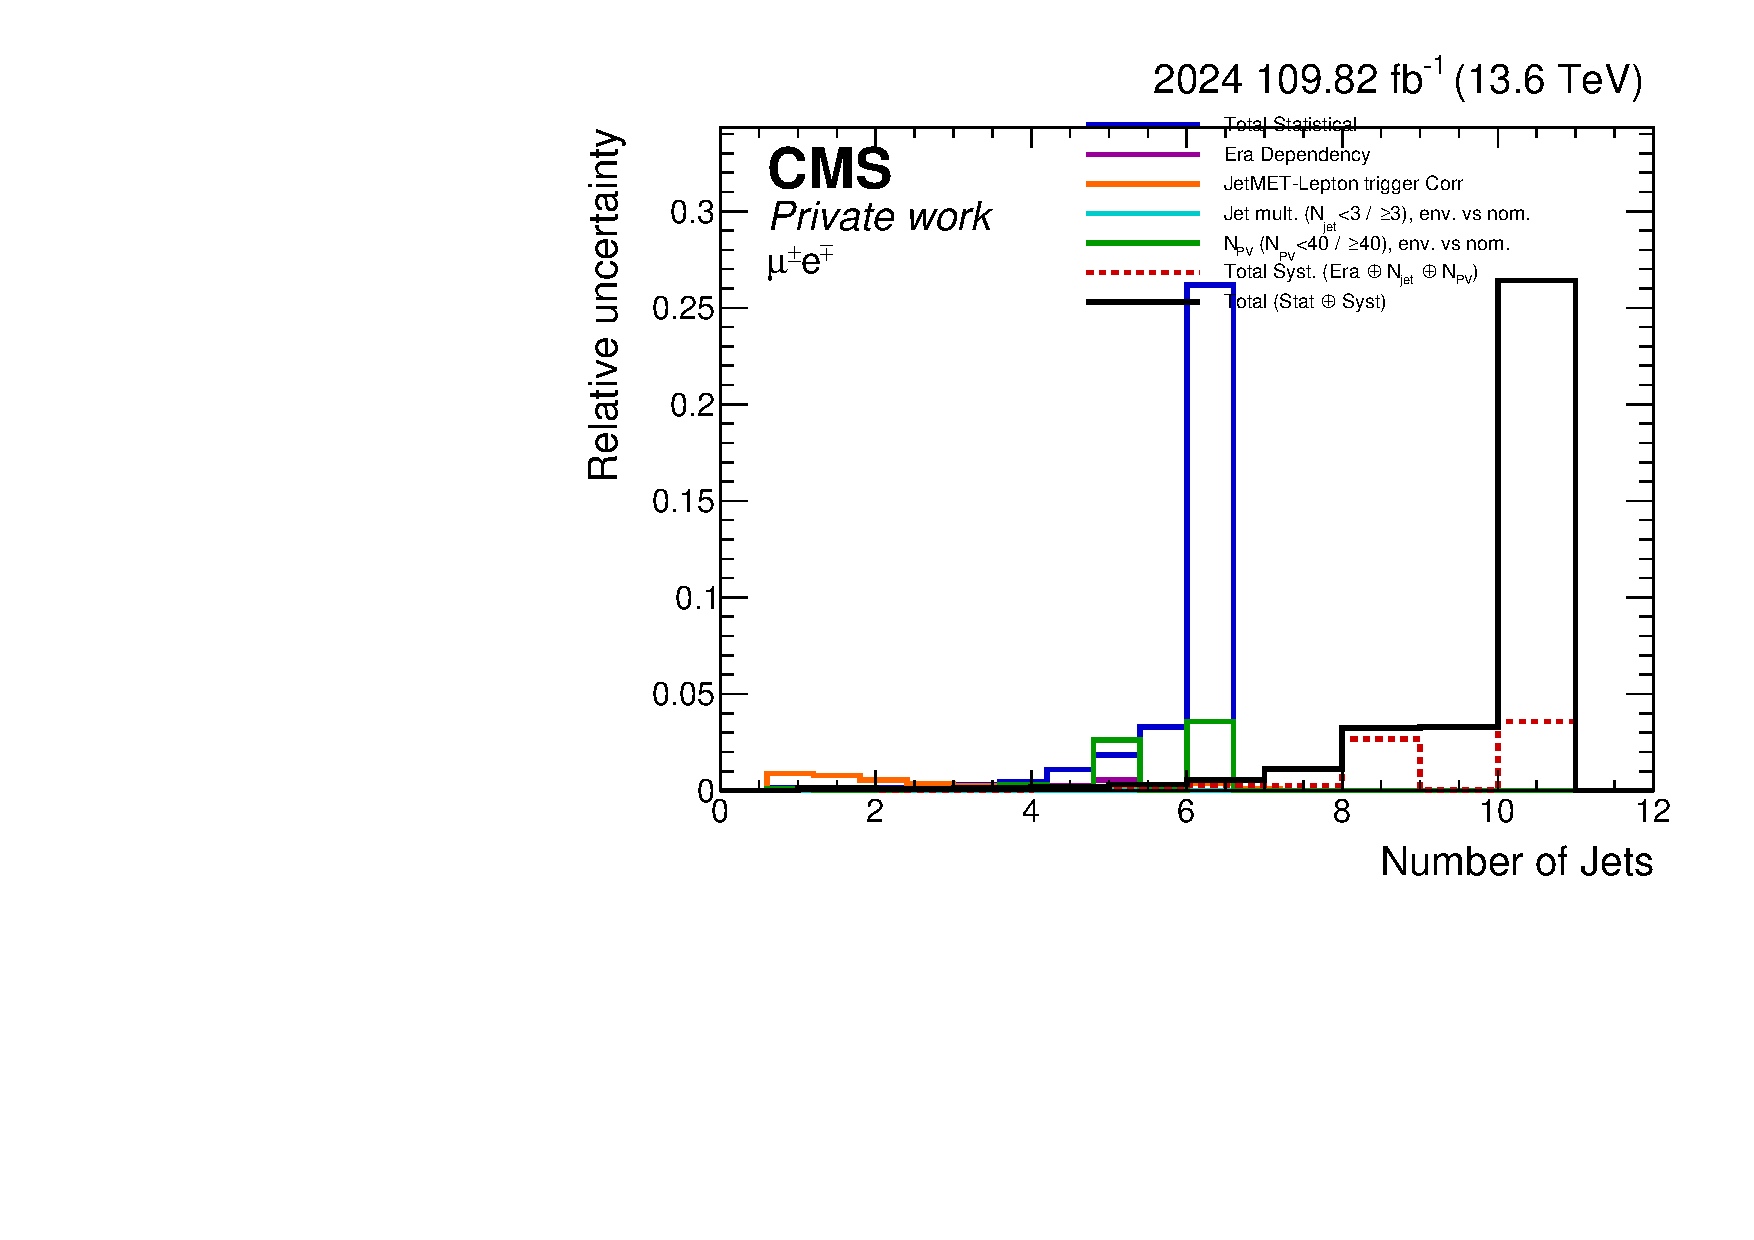
\includegraphics[width=0.48\linewidth]{figures/2024/MuEl/Relative_Uncertainty_Breakdown/Breakdown_Num_Jets.pdf}
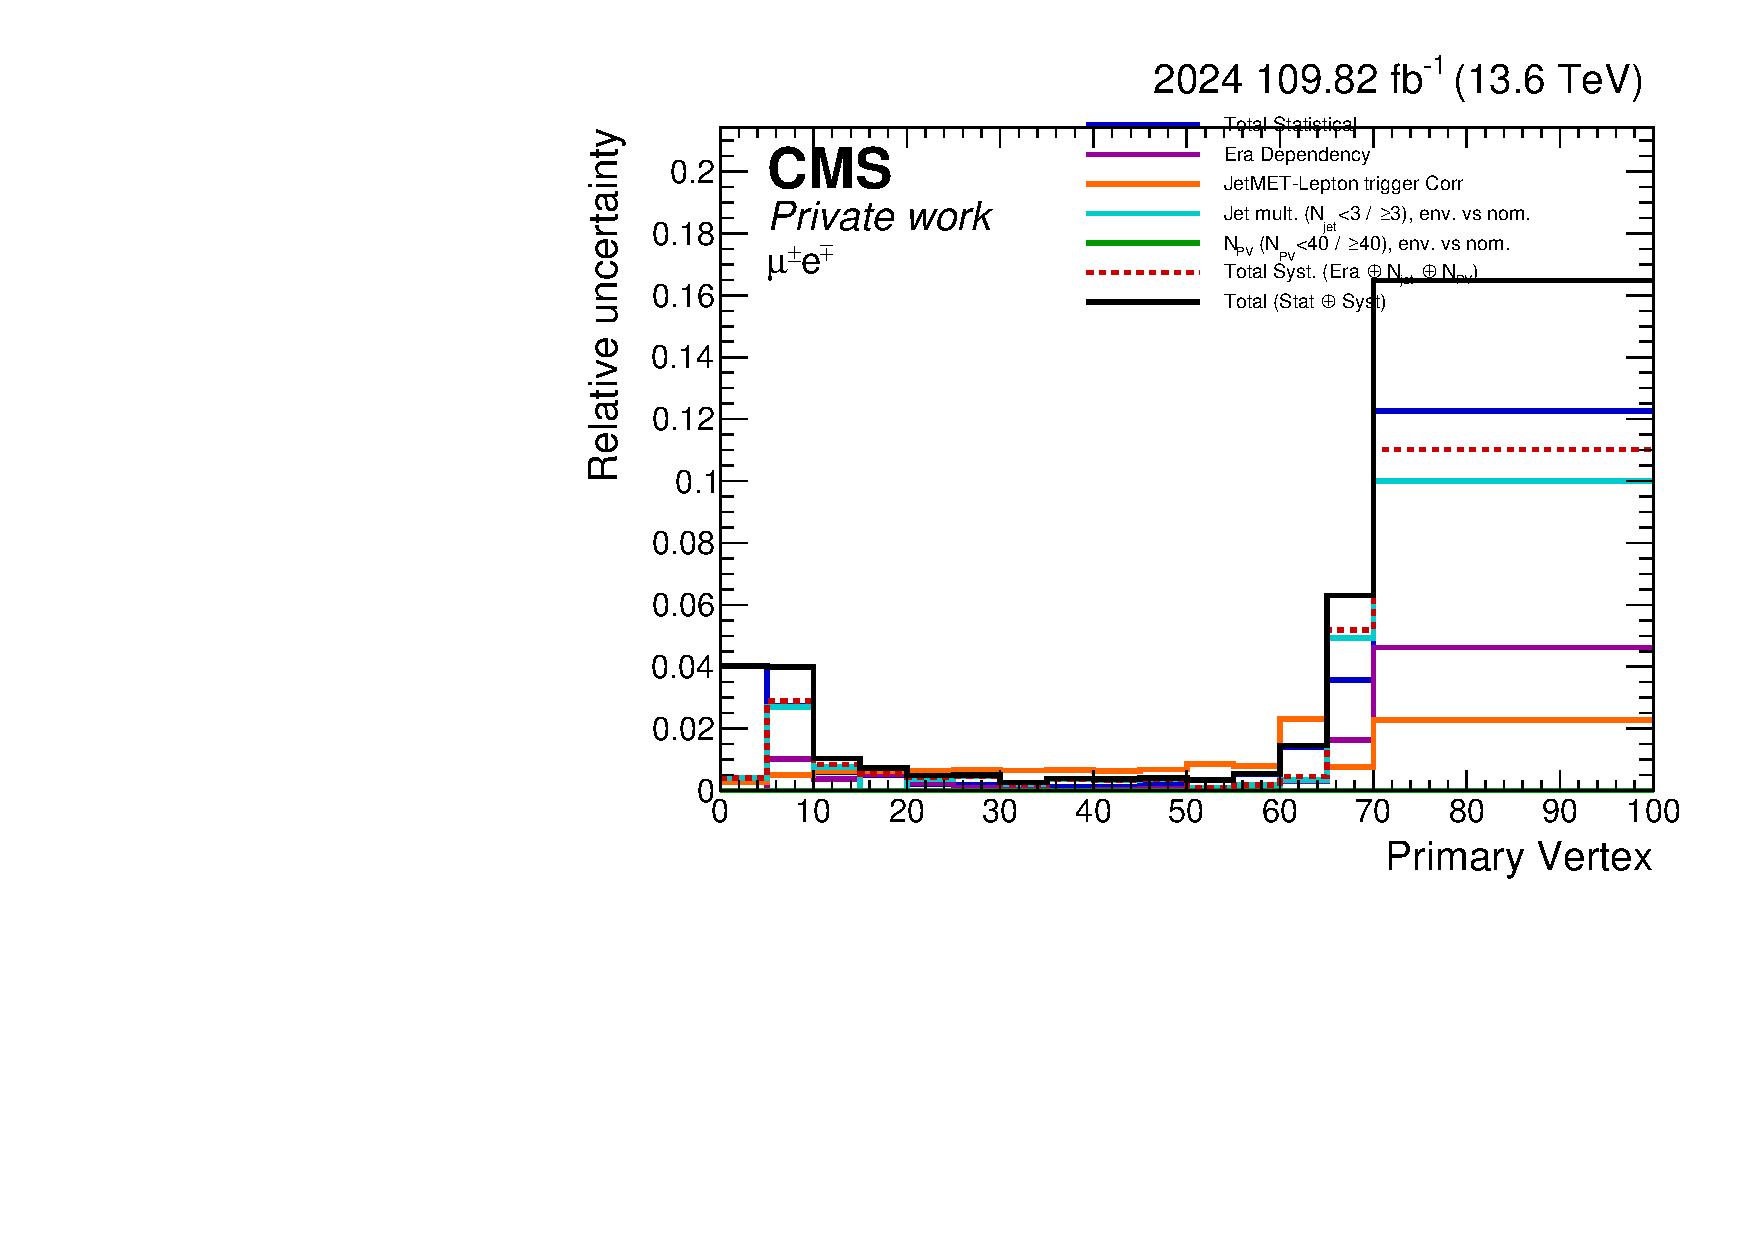
\includegraphics[width=0.48\linewidth]{figures/2024/MuEl/Relative_Uncertainty_Breakdown/Breakdown_Num_PV.pdf}
\caption{Relative uncertainty component breakdown versus event activity in the $e\mu$ channel. Left and right: jet and primary-vertex multiplicities.}\label{fig:extra-MuEl-Relative-Uncertainty-Breakdown-Num_Jets}\end{figure}
\begin{figure}[p]\centering
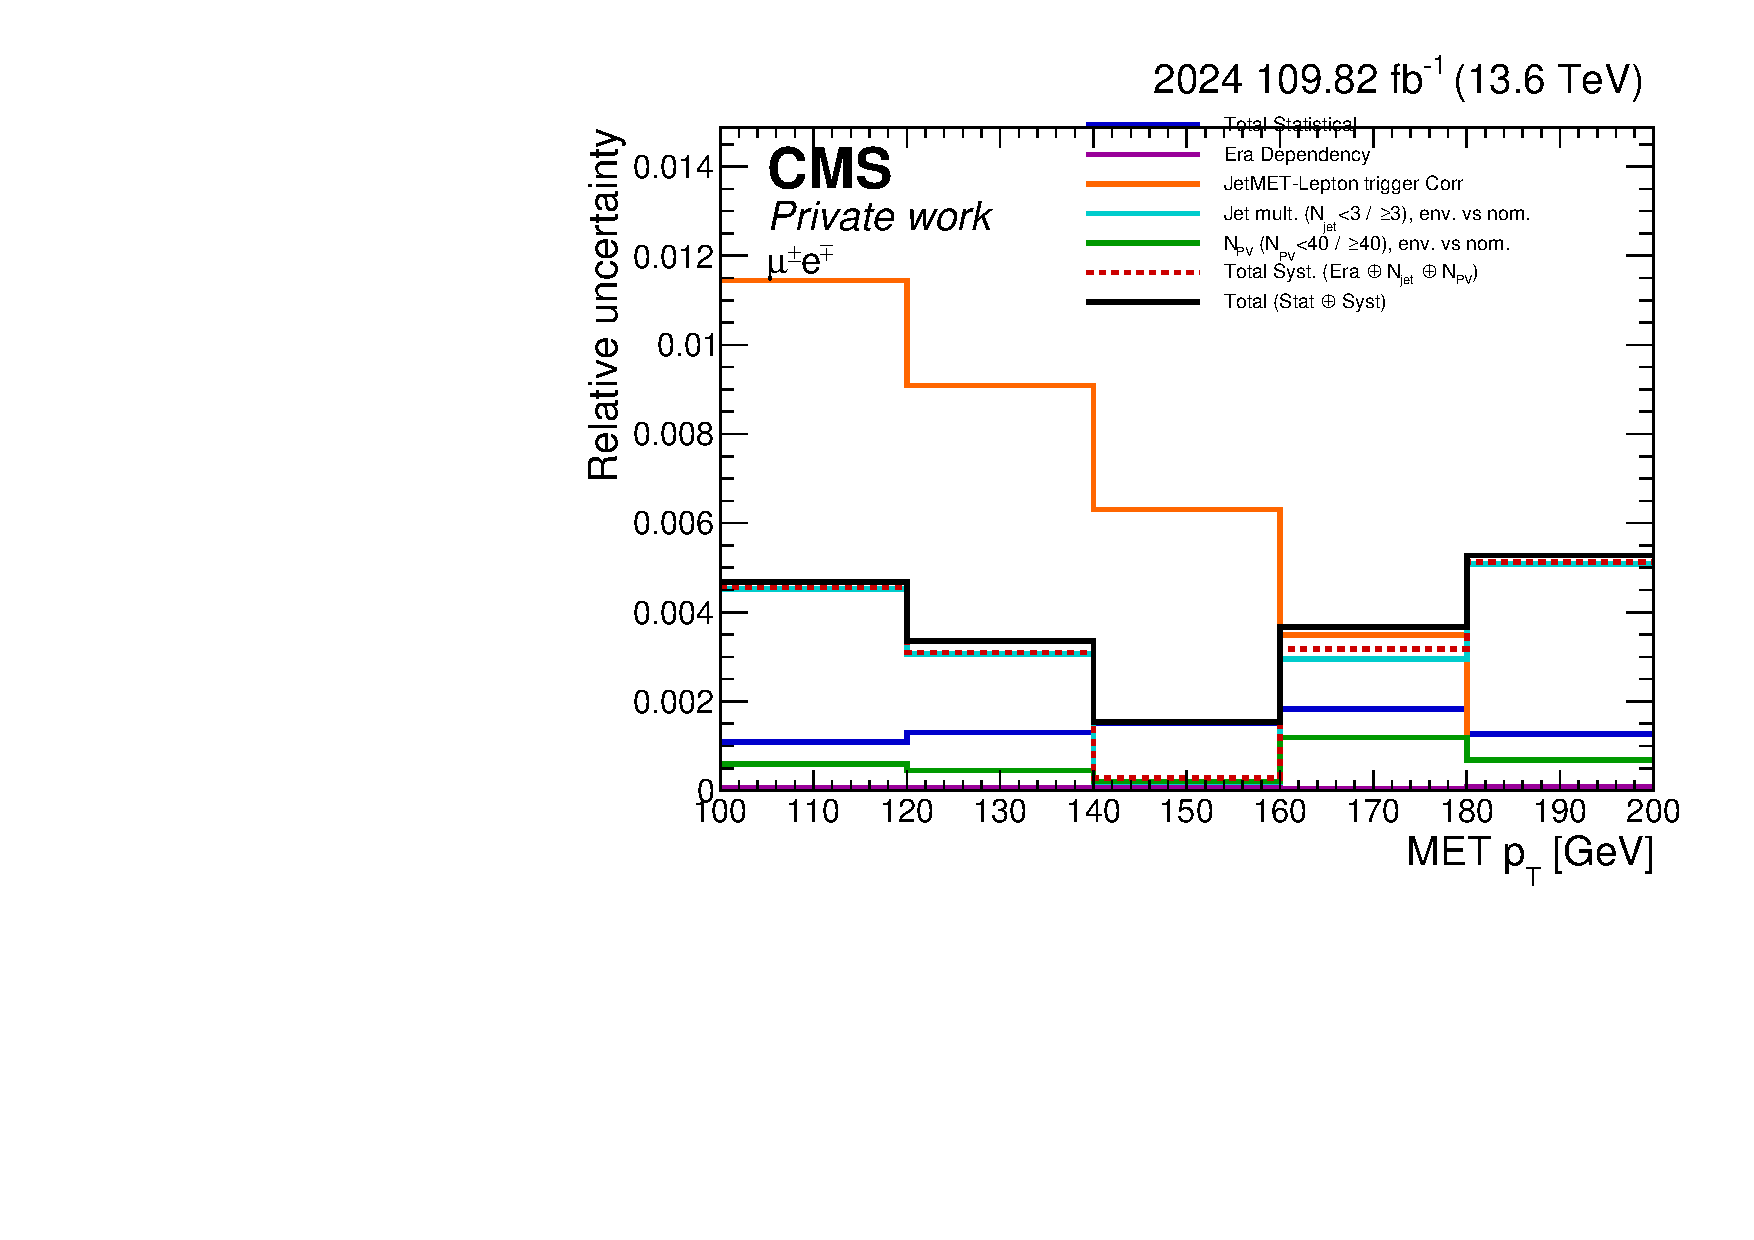
\includegraphics[width=0.48\linewidth]{figures/2024/MuEl/Relative_Uncertainty_Breakdown/Breakdown_METpt.pdf}
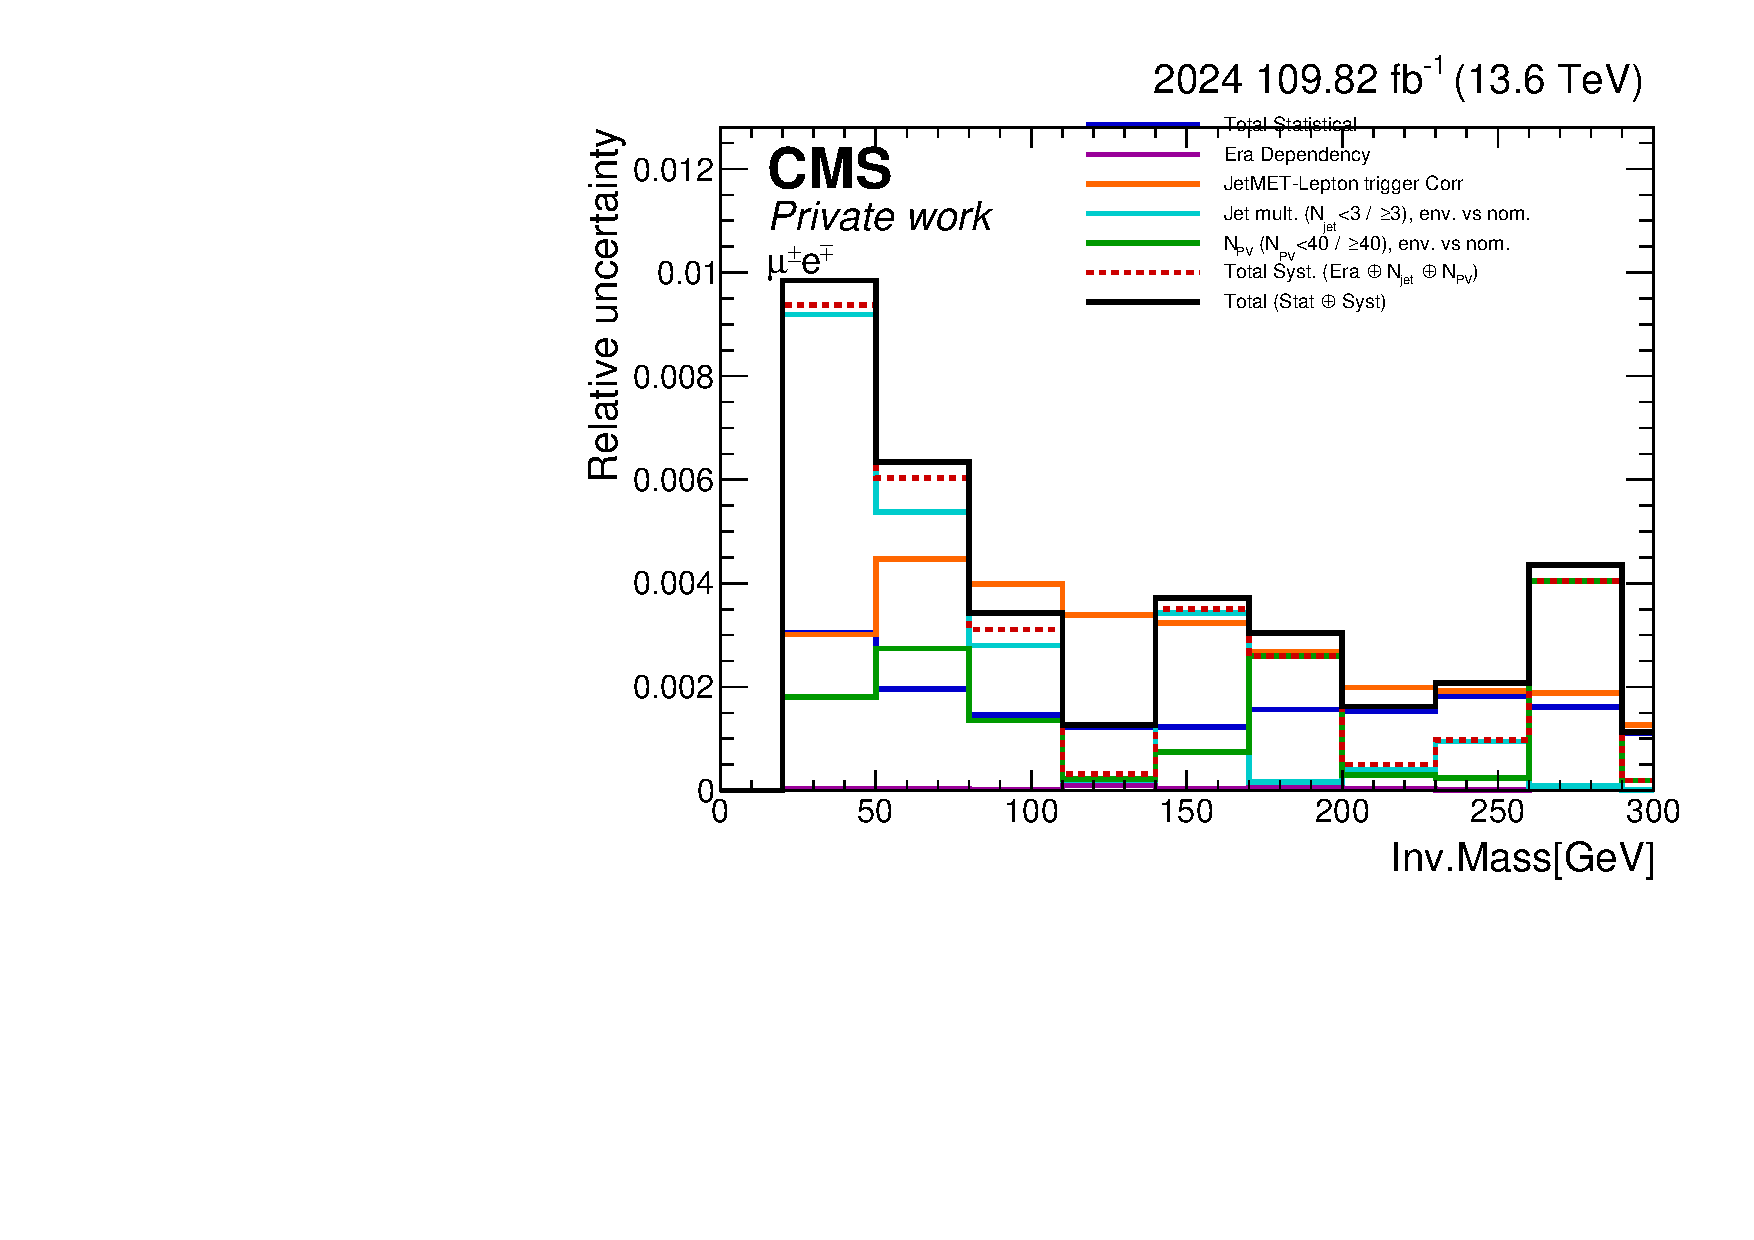
\includegraphics[width=0.48\linewidth]{figures/2024/MuEl/Relative_Uncertainty_Breakdown/Breakdown_DiLepMass.pdf}
\caption{Relative uncertainty component breakdown versus event kinematics in the $e\mu$ channel. Left and right: missing transverse momentum and dilepton invariant mass.}\label{fig:extra-MuEl-Relative-Uncertainty-Breakdown-METpt}\end{figure}
\begin{figure}[p]\centering
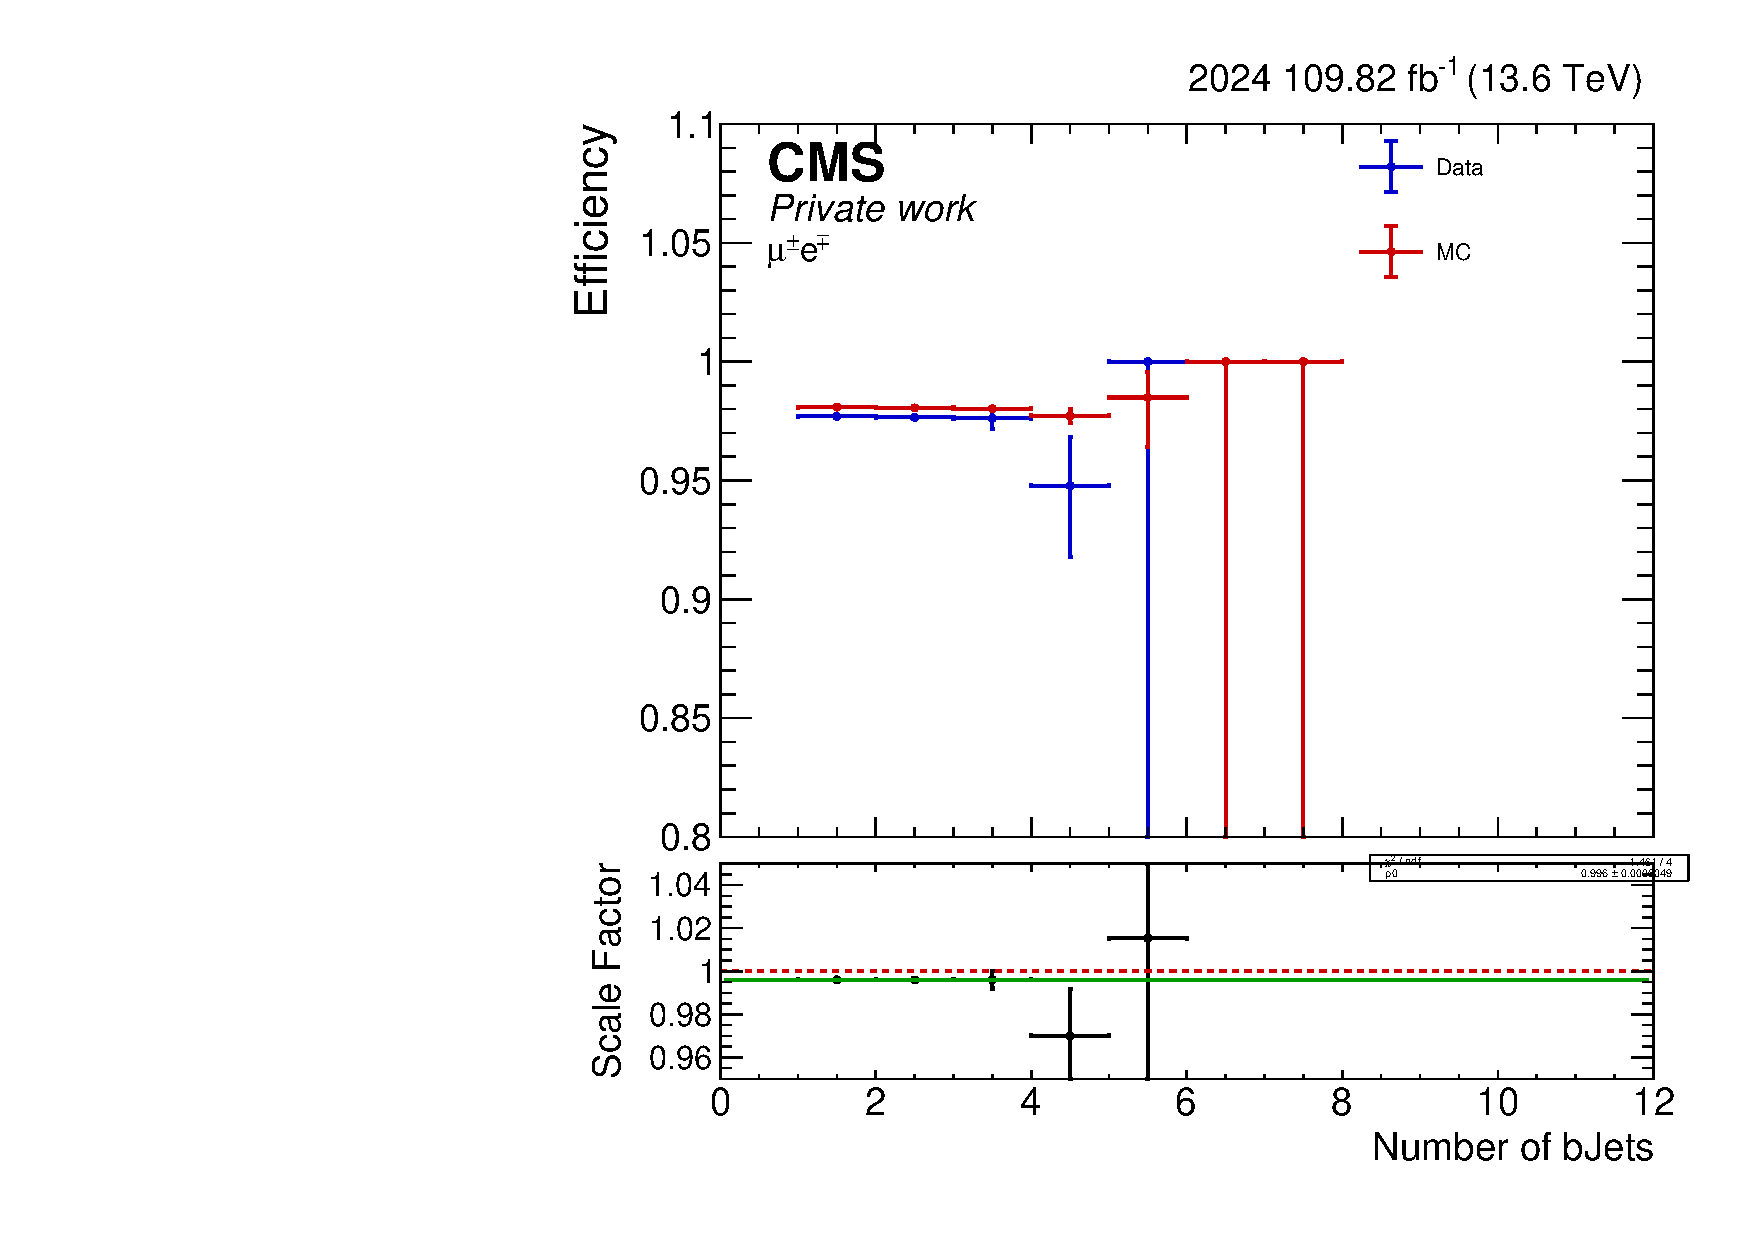
\includegraphics[width=0.48\linewidth]{figures/2024/MuEl/ScaleFactor/SF_Num_bJets.pdf}
\caption{Efficiency comparison and scale factor versus heavy-flavour activity in the $e\mu$ channel. $b$-tagged jet multiplicity.}\label{fig:extra-MuEl-ScaleFactor-Num_bJets}\end{figure}
\begin{figure}[p]\centering
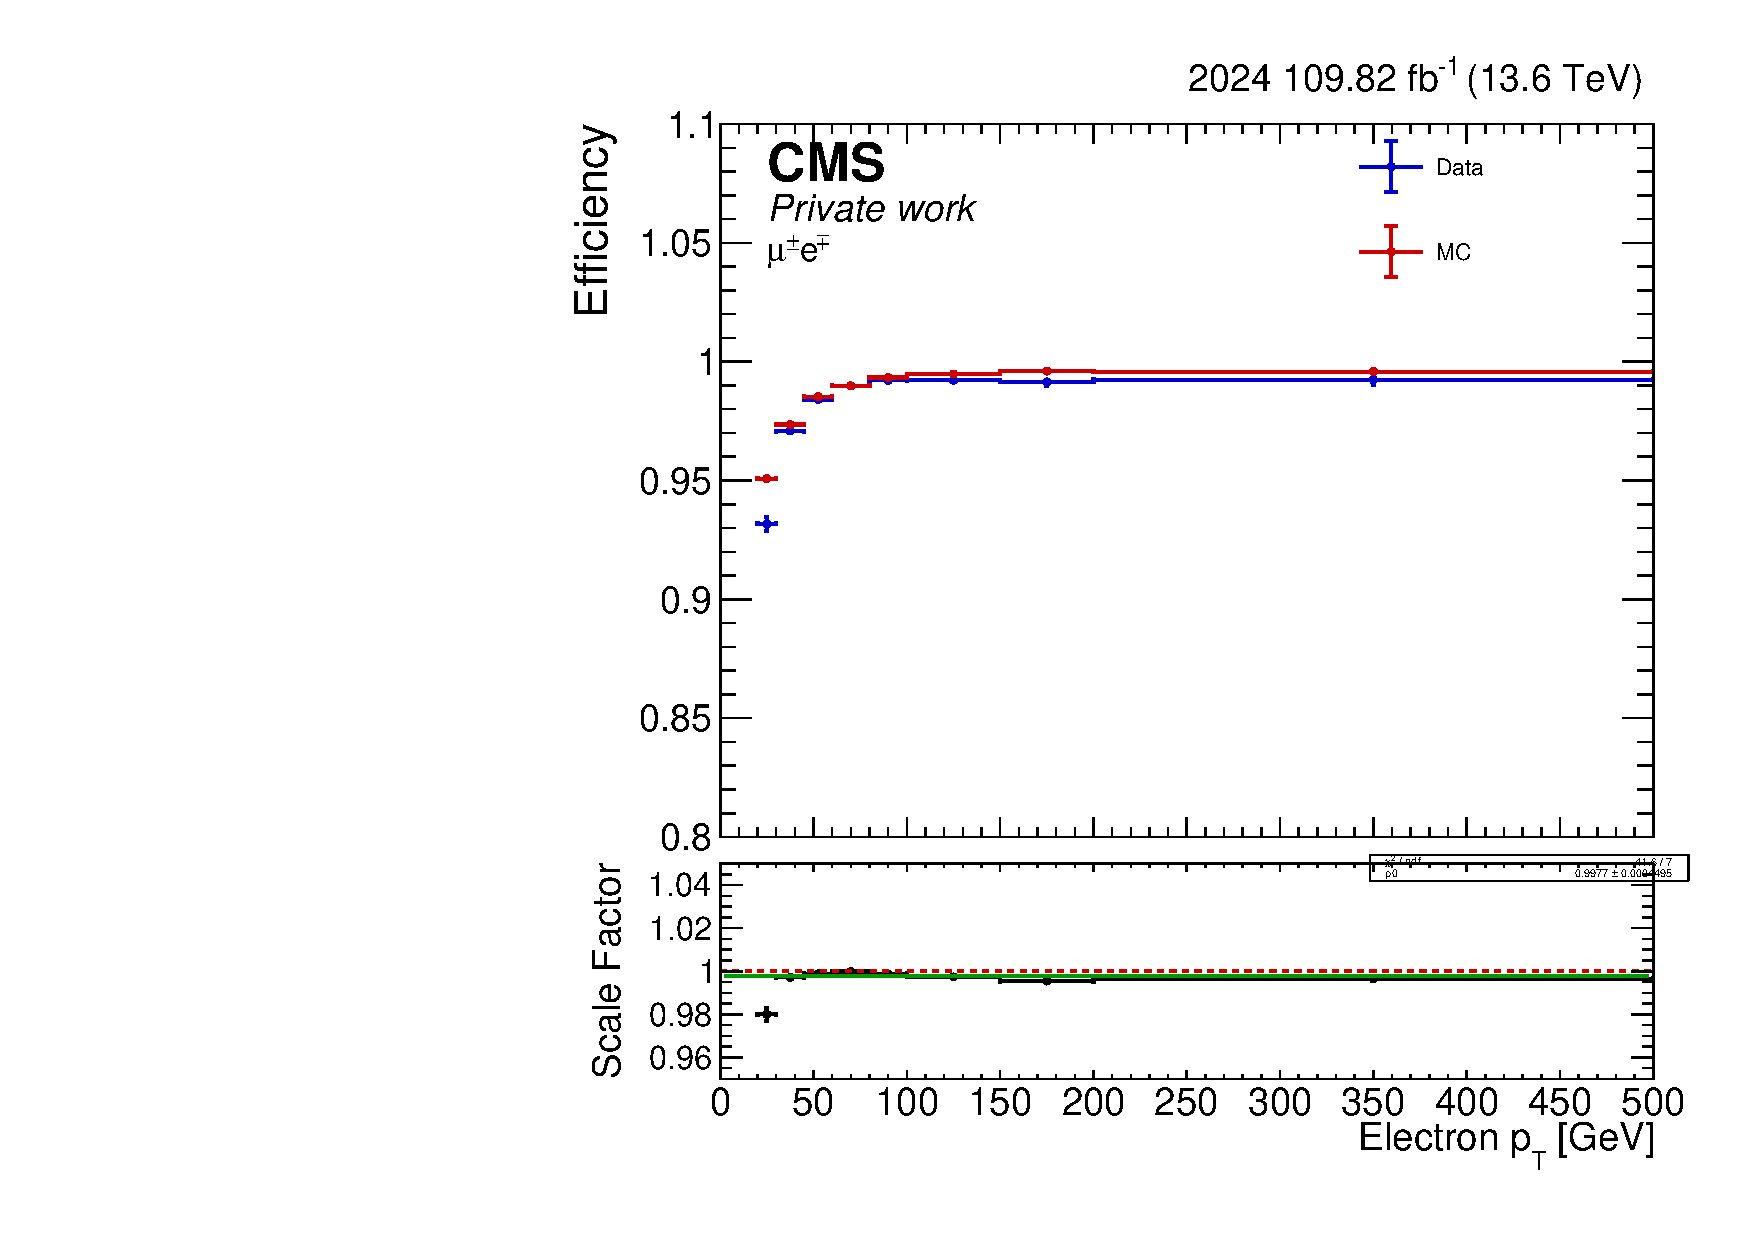
\includegraphics[width=0.48\linewidth]{figures/2024/MuEl/ScaleFactor/SF_ElPt.pdf}
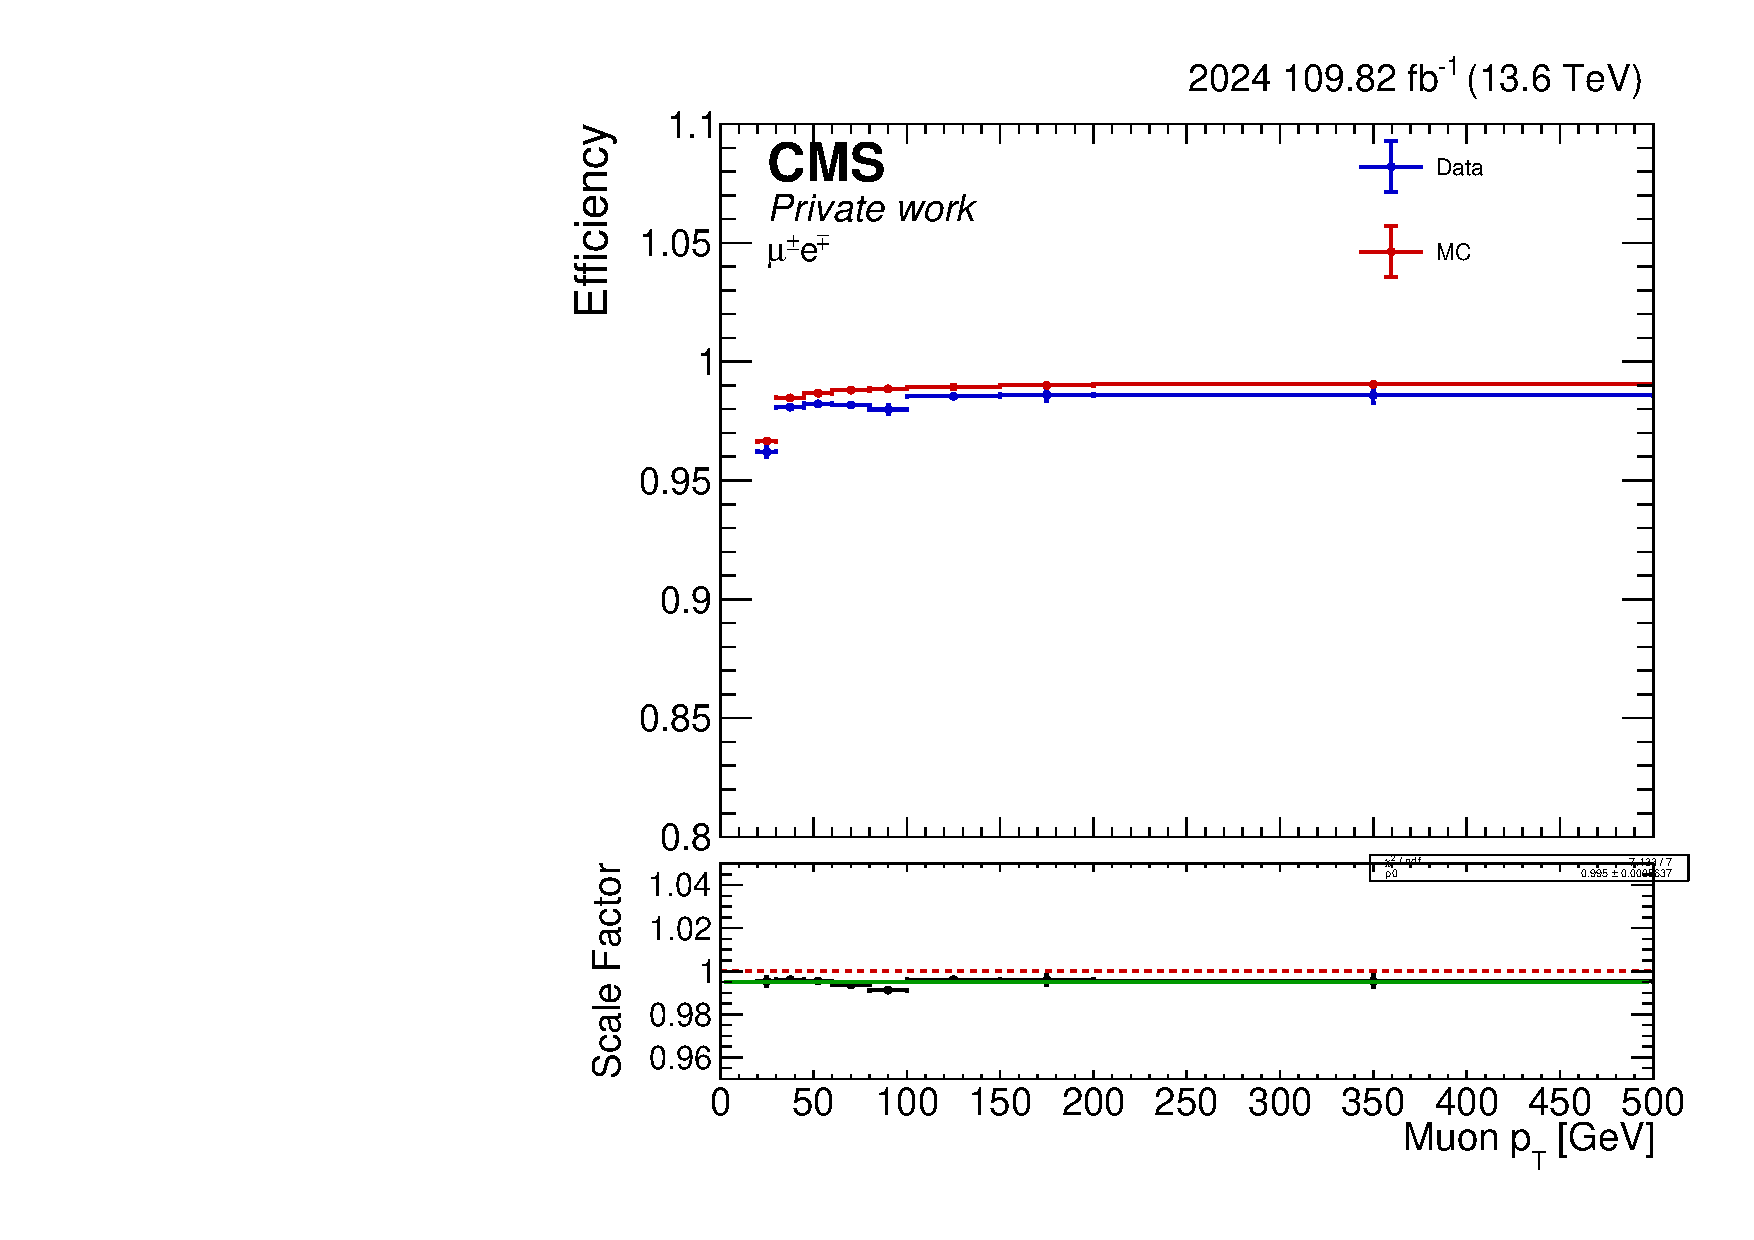
\includegraphics[width=0.48\linewidth]{figures/2024/MuEl/ScaleFactor/SF_MuPt.pdf}
\caption{Efficiency comparison and scale factor in the flavour-specific momentum variables used by the two-dimensional correction in the $e\mu$ channel. Left and right: electron and muon $p_{\mathrm{T}}$.}\label{fig:extra-MuEl-ScaleFactor-ElPt}\end{figure}
\clearpage\subsection{$\mu\mu$ channel}
\begin{figure}[p]\centering
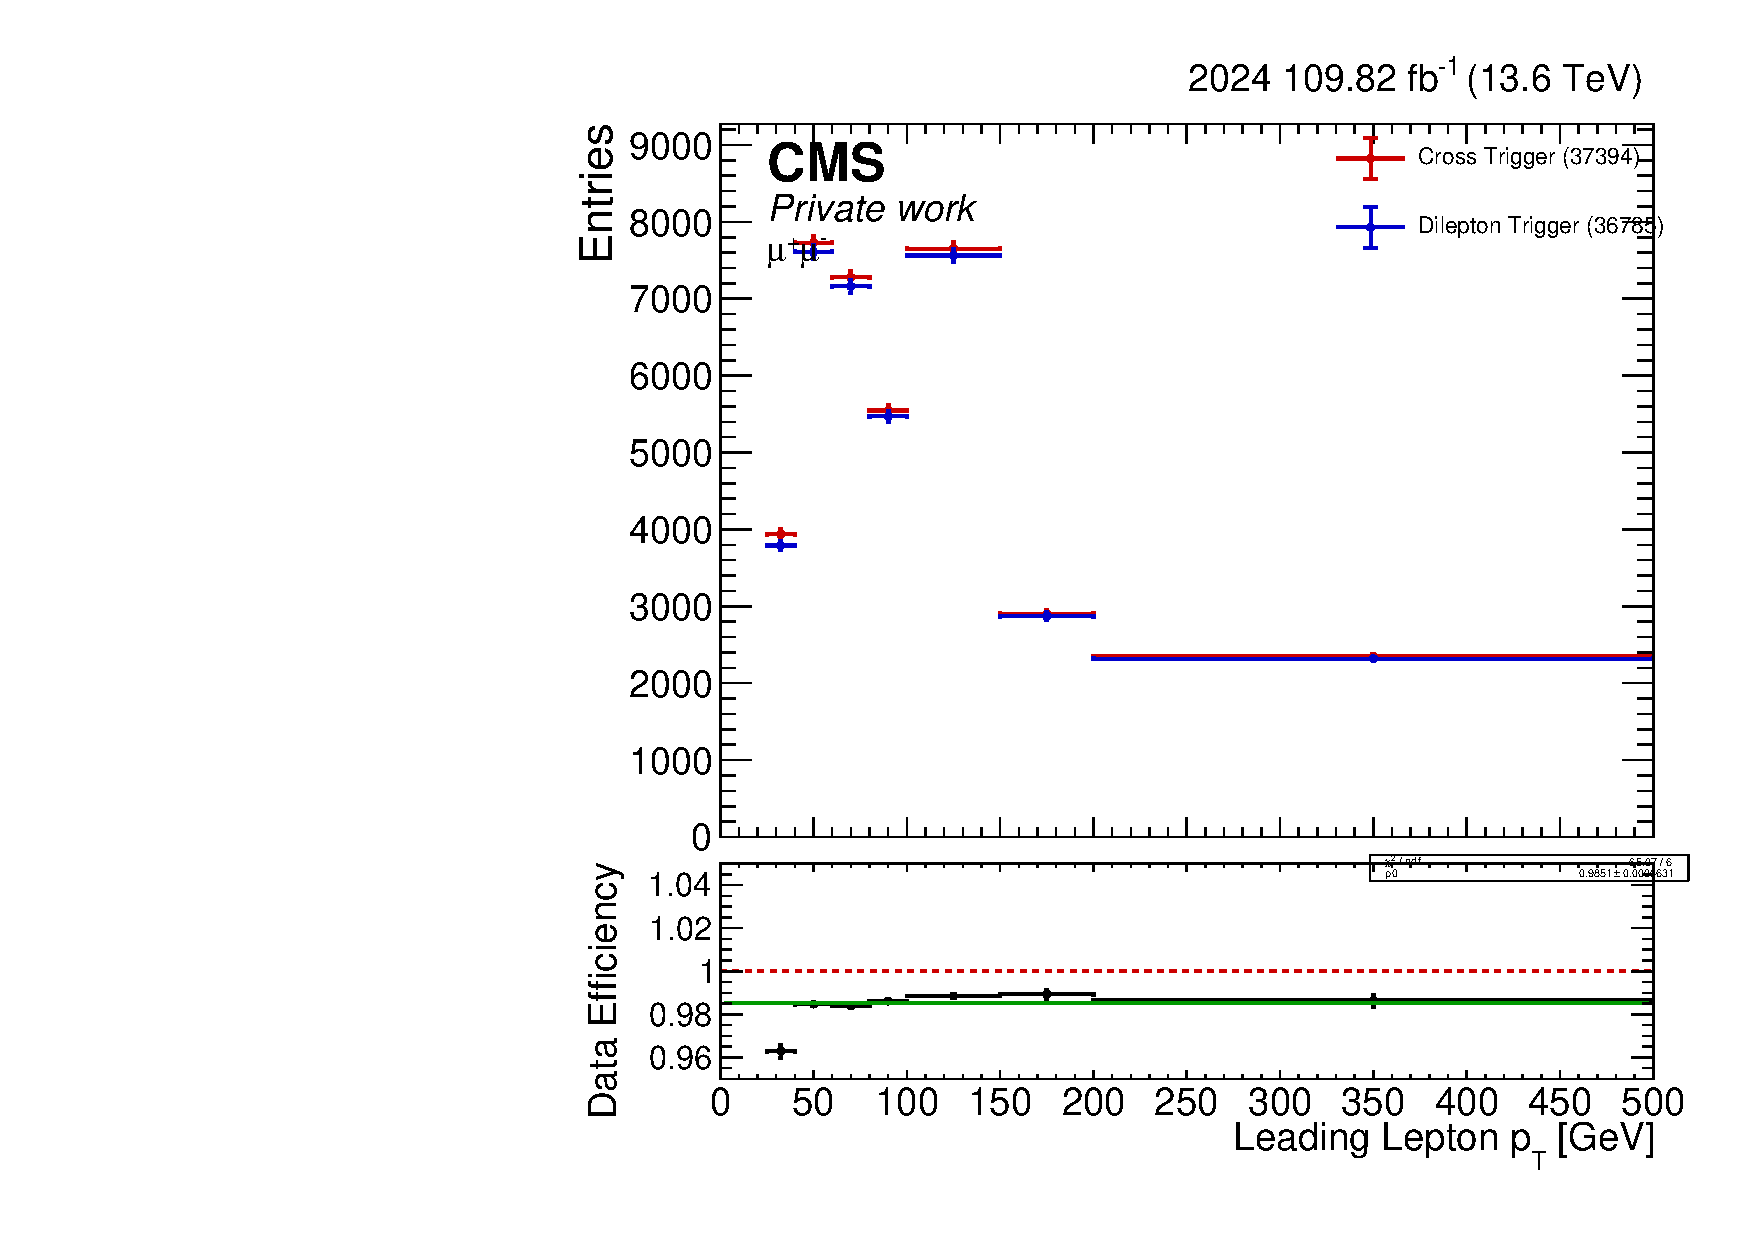
\includegraphics[width=0.48\linewidth]{figures/2024/MuMu/TrigEffData/TrigEff_Lep1pt.pdf}
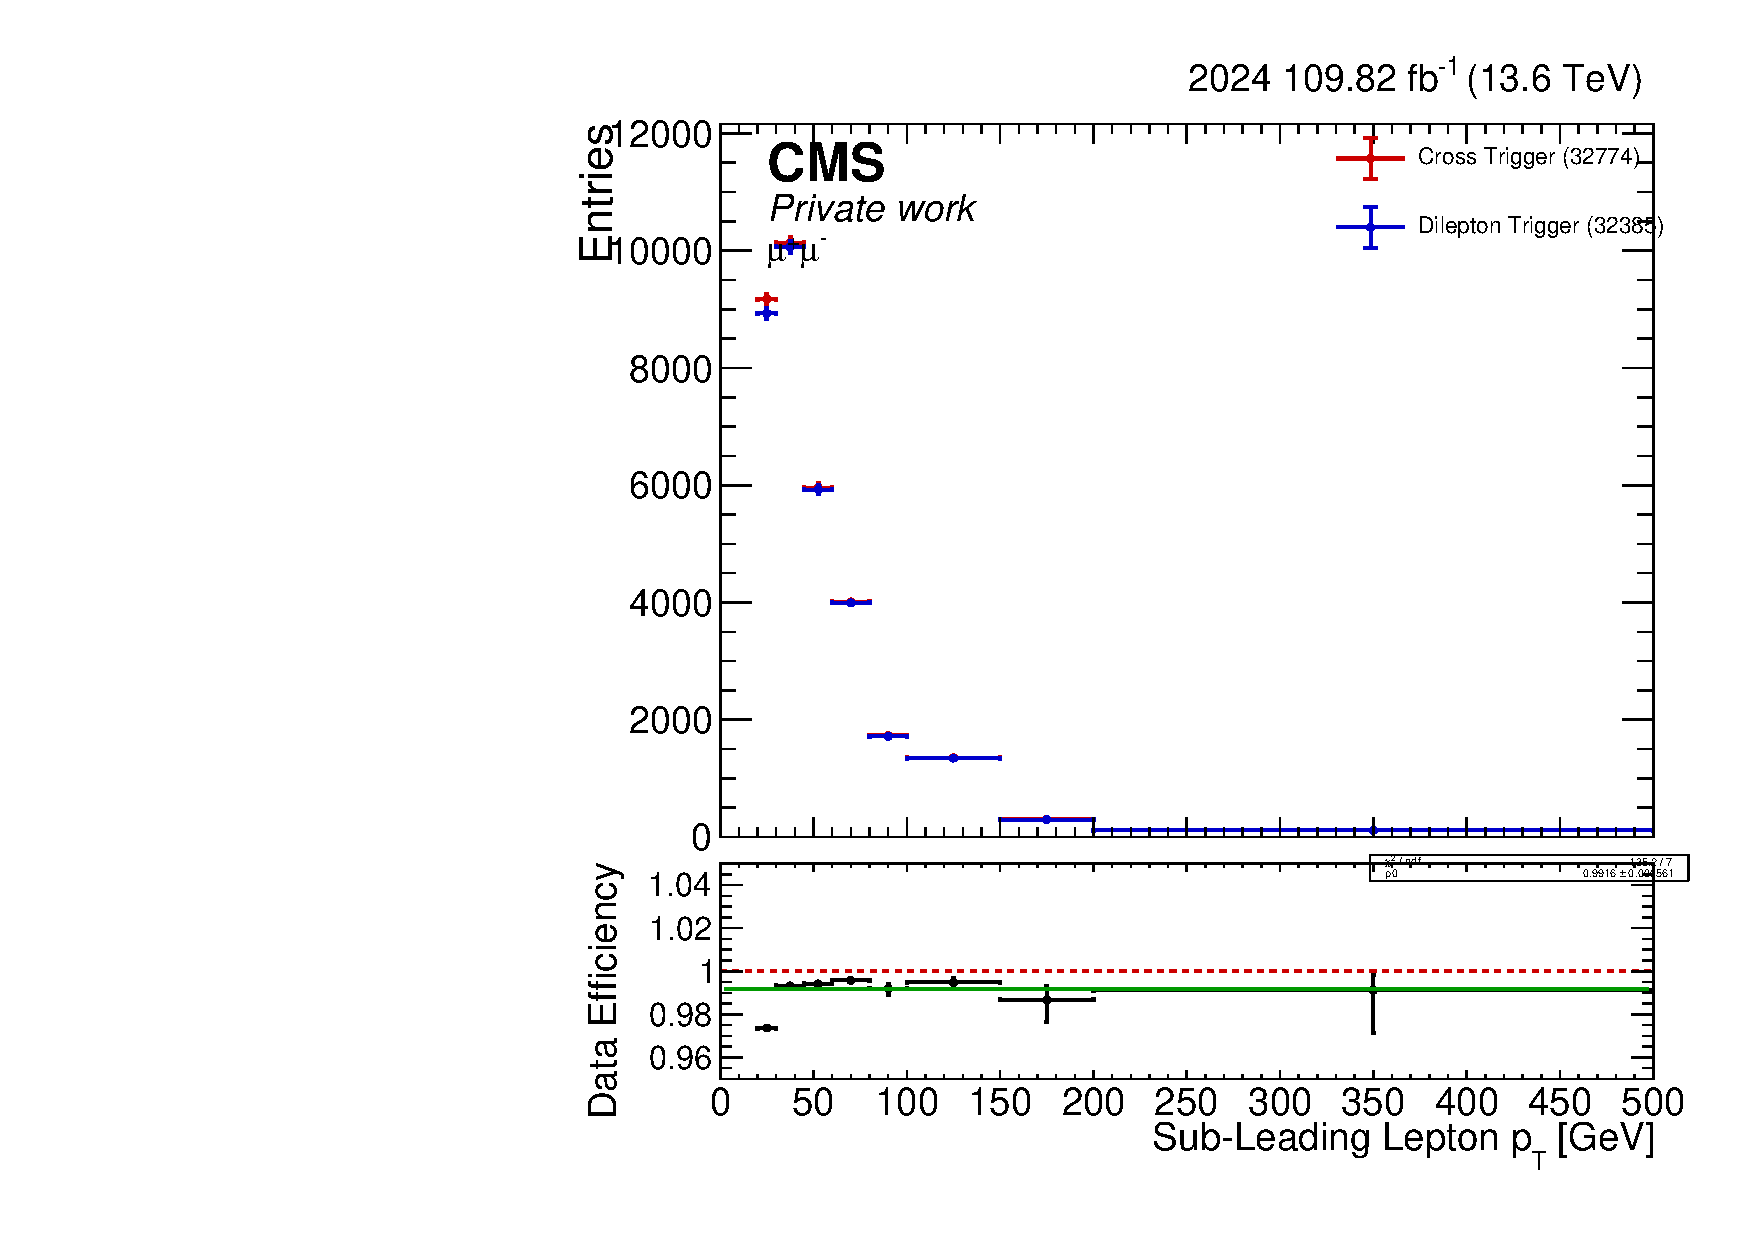
\includegraphics[width=0.48\linewidth]{figures/2024/MuMu/TrigEffData/TrigEff_Lep2pt.pdf}
\caption{Data trigger numerator and reference-sample distributions (upper panels), with their efficiency ratios (lower panels) in the $\mu\mu$ channel. Left and right: leading and subleading lepton $p_{\mathrm{T}}$.}\label{fig:extra-MuMu-TrigEffData-Lep1pt}\end{figure}
\begin{figure}[p]\centering
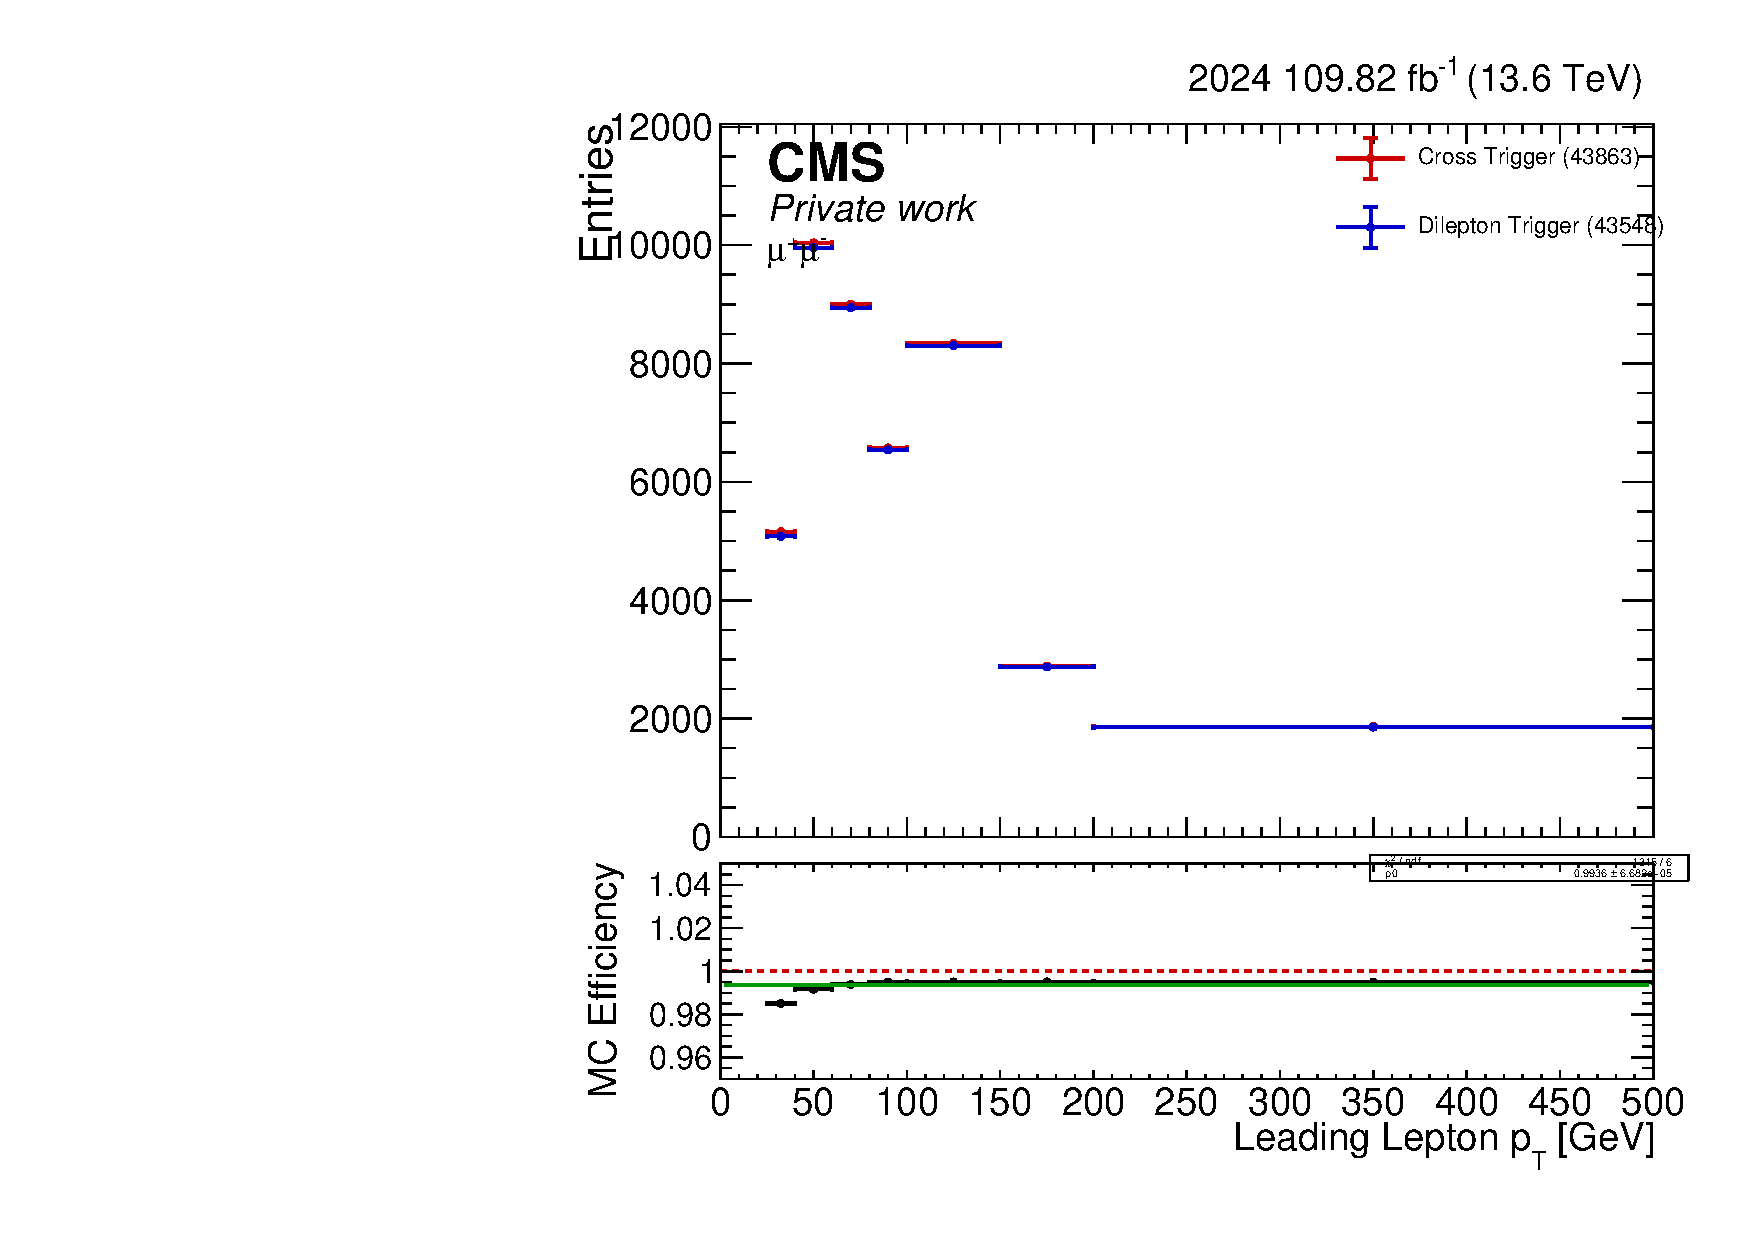
\includegraphics[width=0.48\linewidth]{figures/2024/MuMu/TrigEffMC/TrigEff_Lep1pt.pdf}
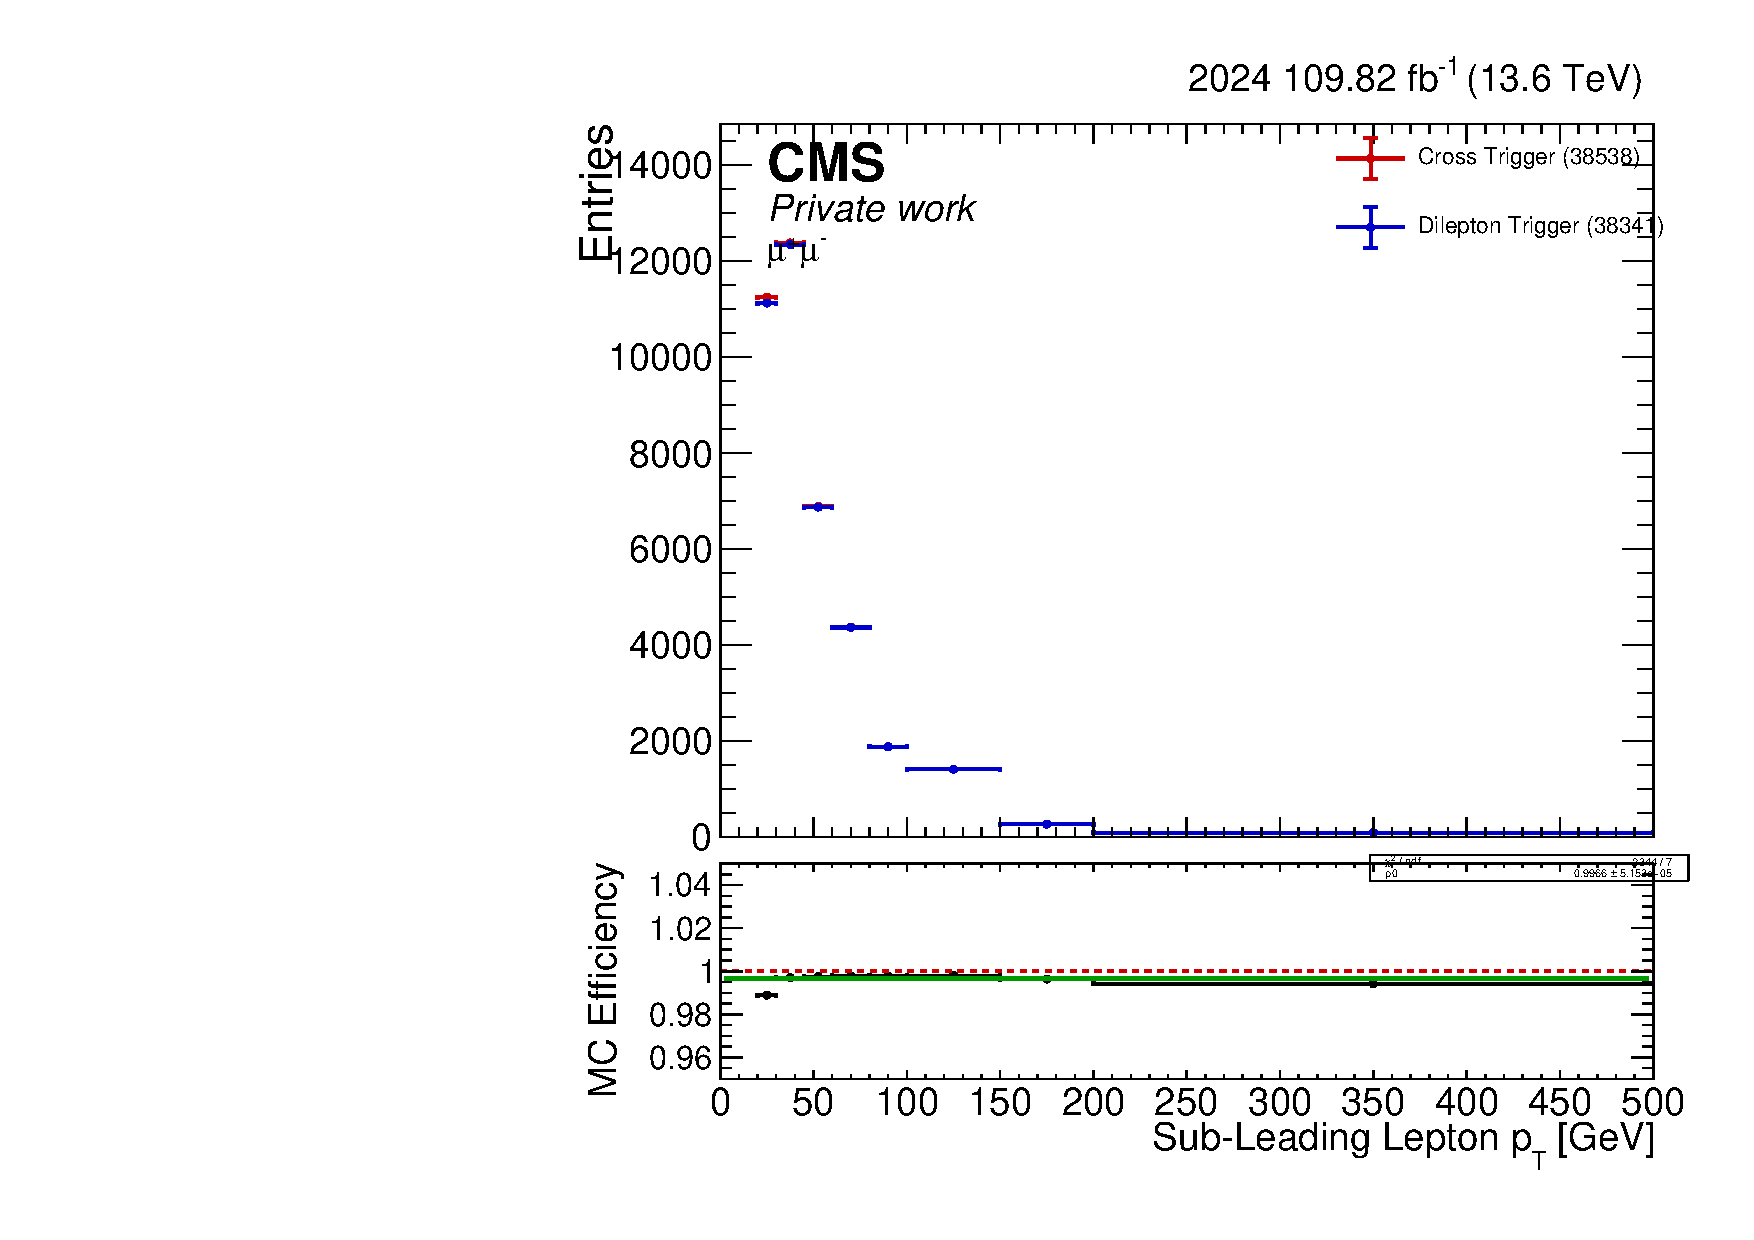
\includegraphics[width=0.48\linewidth]{figures/2024/MuMu/TrigEffMC/TrigEff_Lep2pt.pdf}
\caption{Simulated trigger numerator and reference-sample distributions (upper panels), with their efficiency ratios (lower panels) in the $\mu\mu$ channel. Left and right: leading and subleading lepton $p_{\mathrm{T}}$.}\label{fig:extra-MuMu-TrigEffMC-Lep1pt}\end{figure}
\begin{figure}[p]\centering
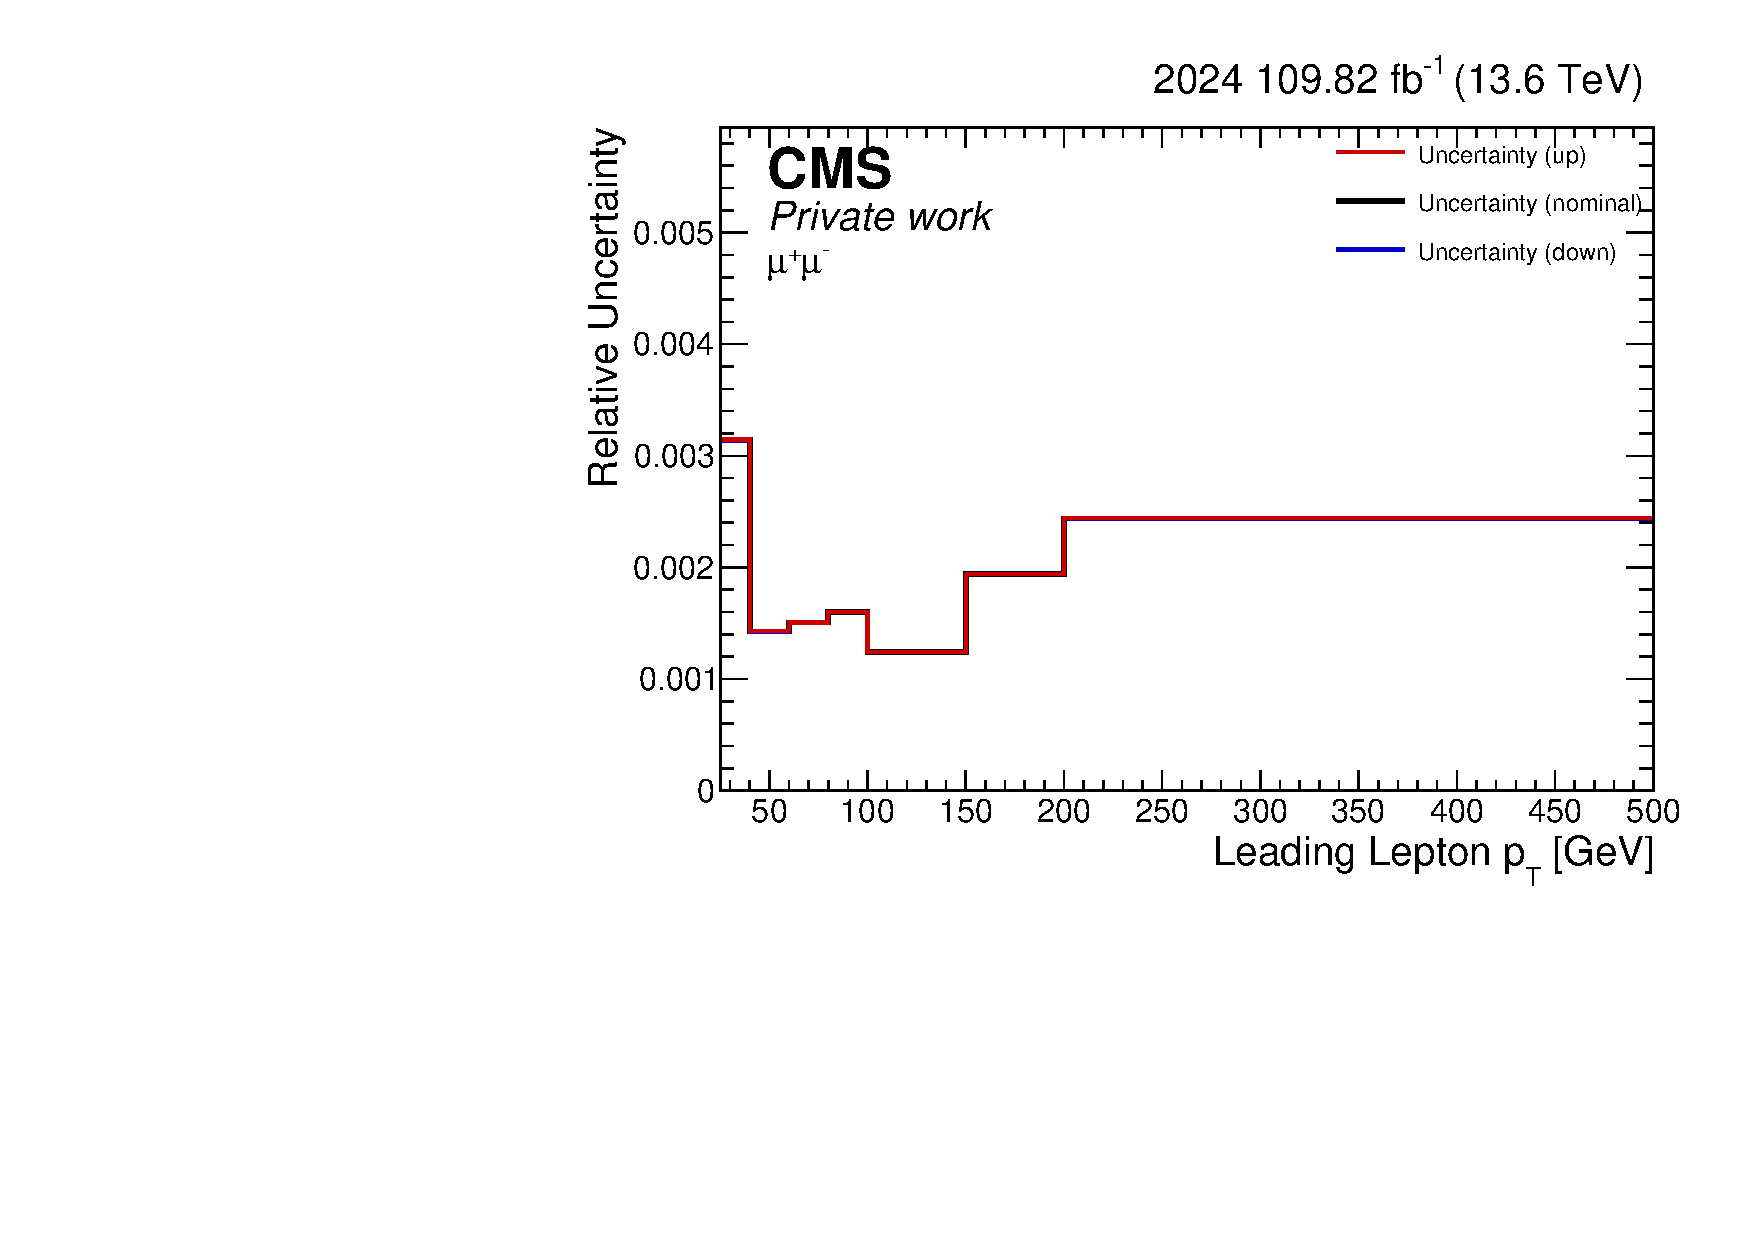
\includegraphics[width=0.48\linewidth]{figures/2024/MuMu/Statistical_Uncertainty/UncRatio_Lep1pt.pdf}
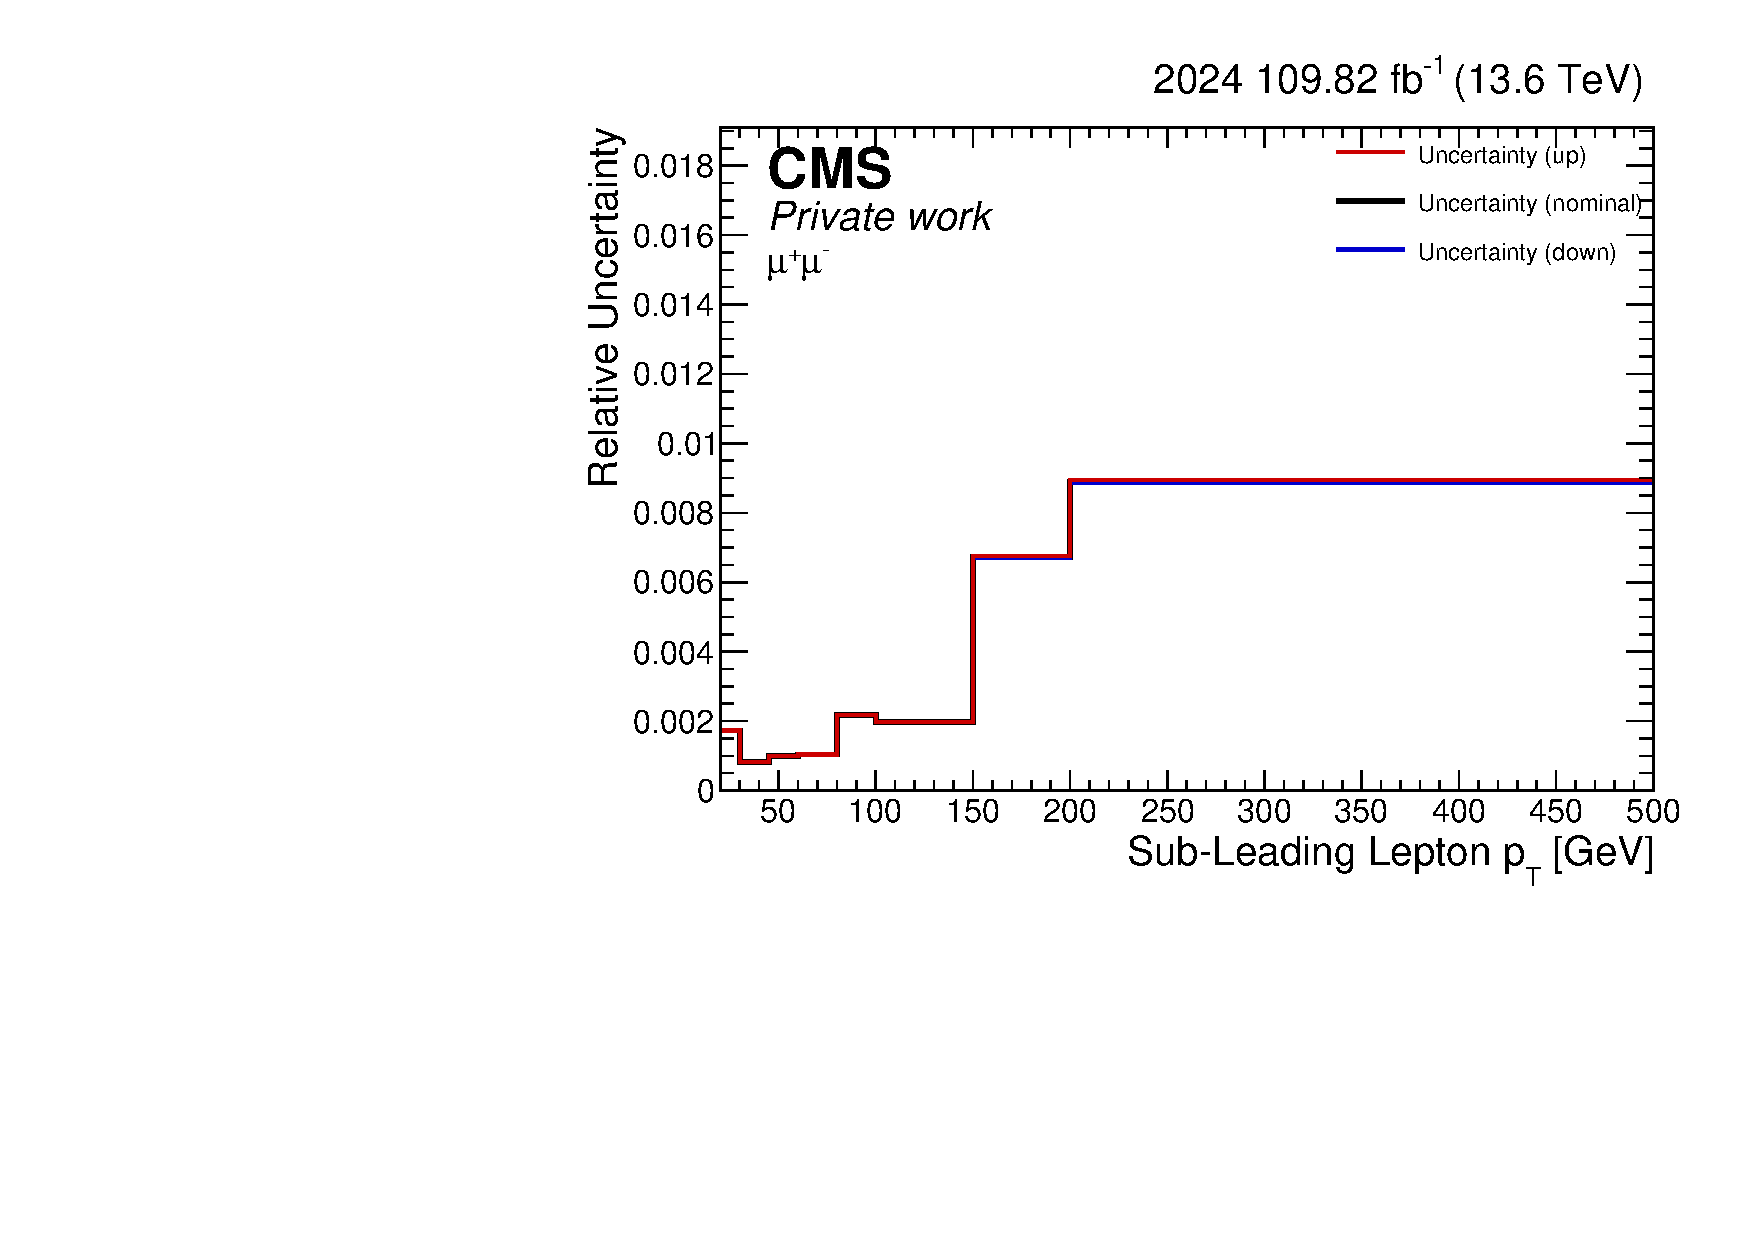
\includegraphics[width=0.48\linewidth]{figures/2024/MuMu/Statistical_Uncertainty/UncRatio_Lep2pt.pdf}
\caption{Relative statistical uncertainty diagnostics, retaining the nominal, upward, and downward curves of the supplied production in the $\mu\mu$ channel. Left and right: leading and subleading lepton $p_{\mathrm{T}}$.}\label{fig:extra-MuMu-Statistical-Uncertainty-Lep1pt}\end{figure}
\begin{figure}[p]\centering
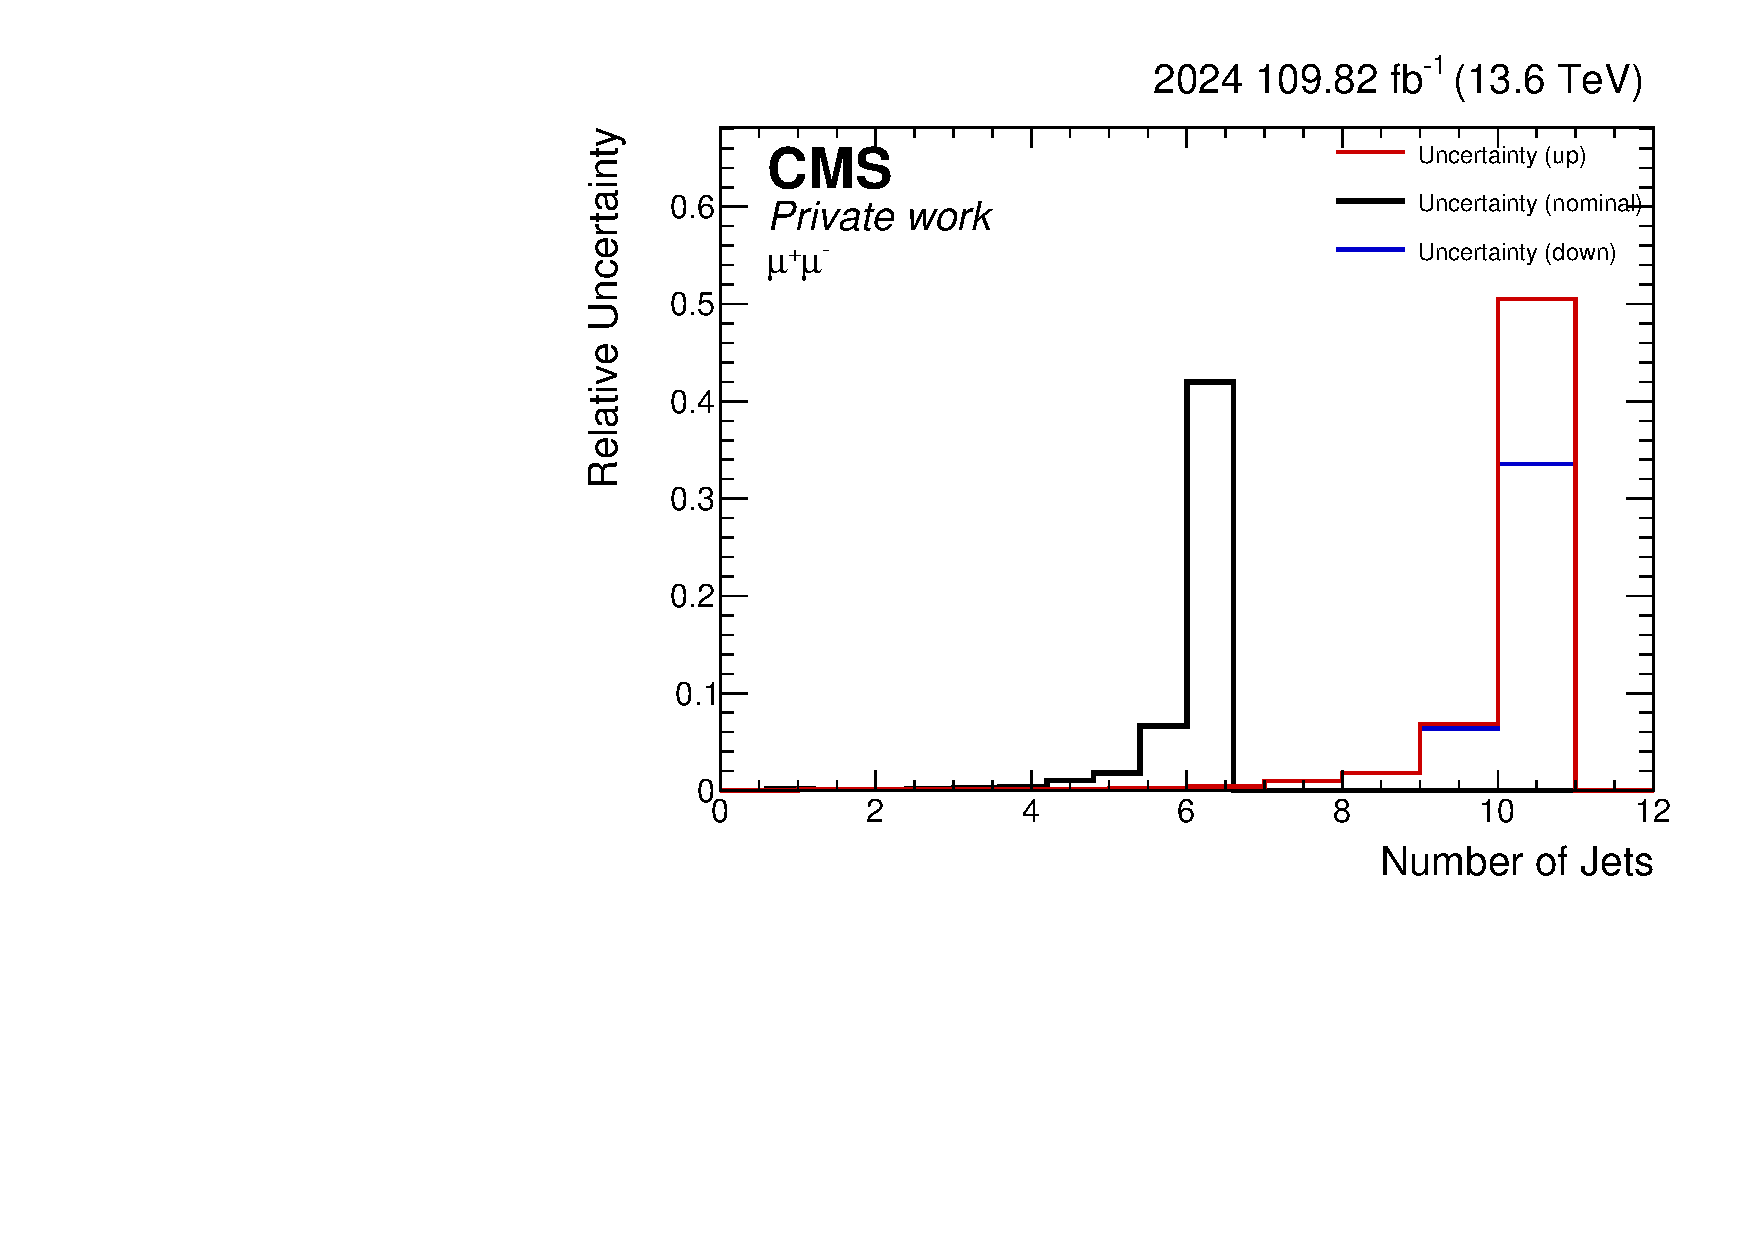
\includegraphics[width=0.48\linewidth]{figures/2024/MuMu/Statistical_Uncertainty/UncRatio_Num_Jets.pdf}
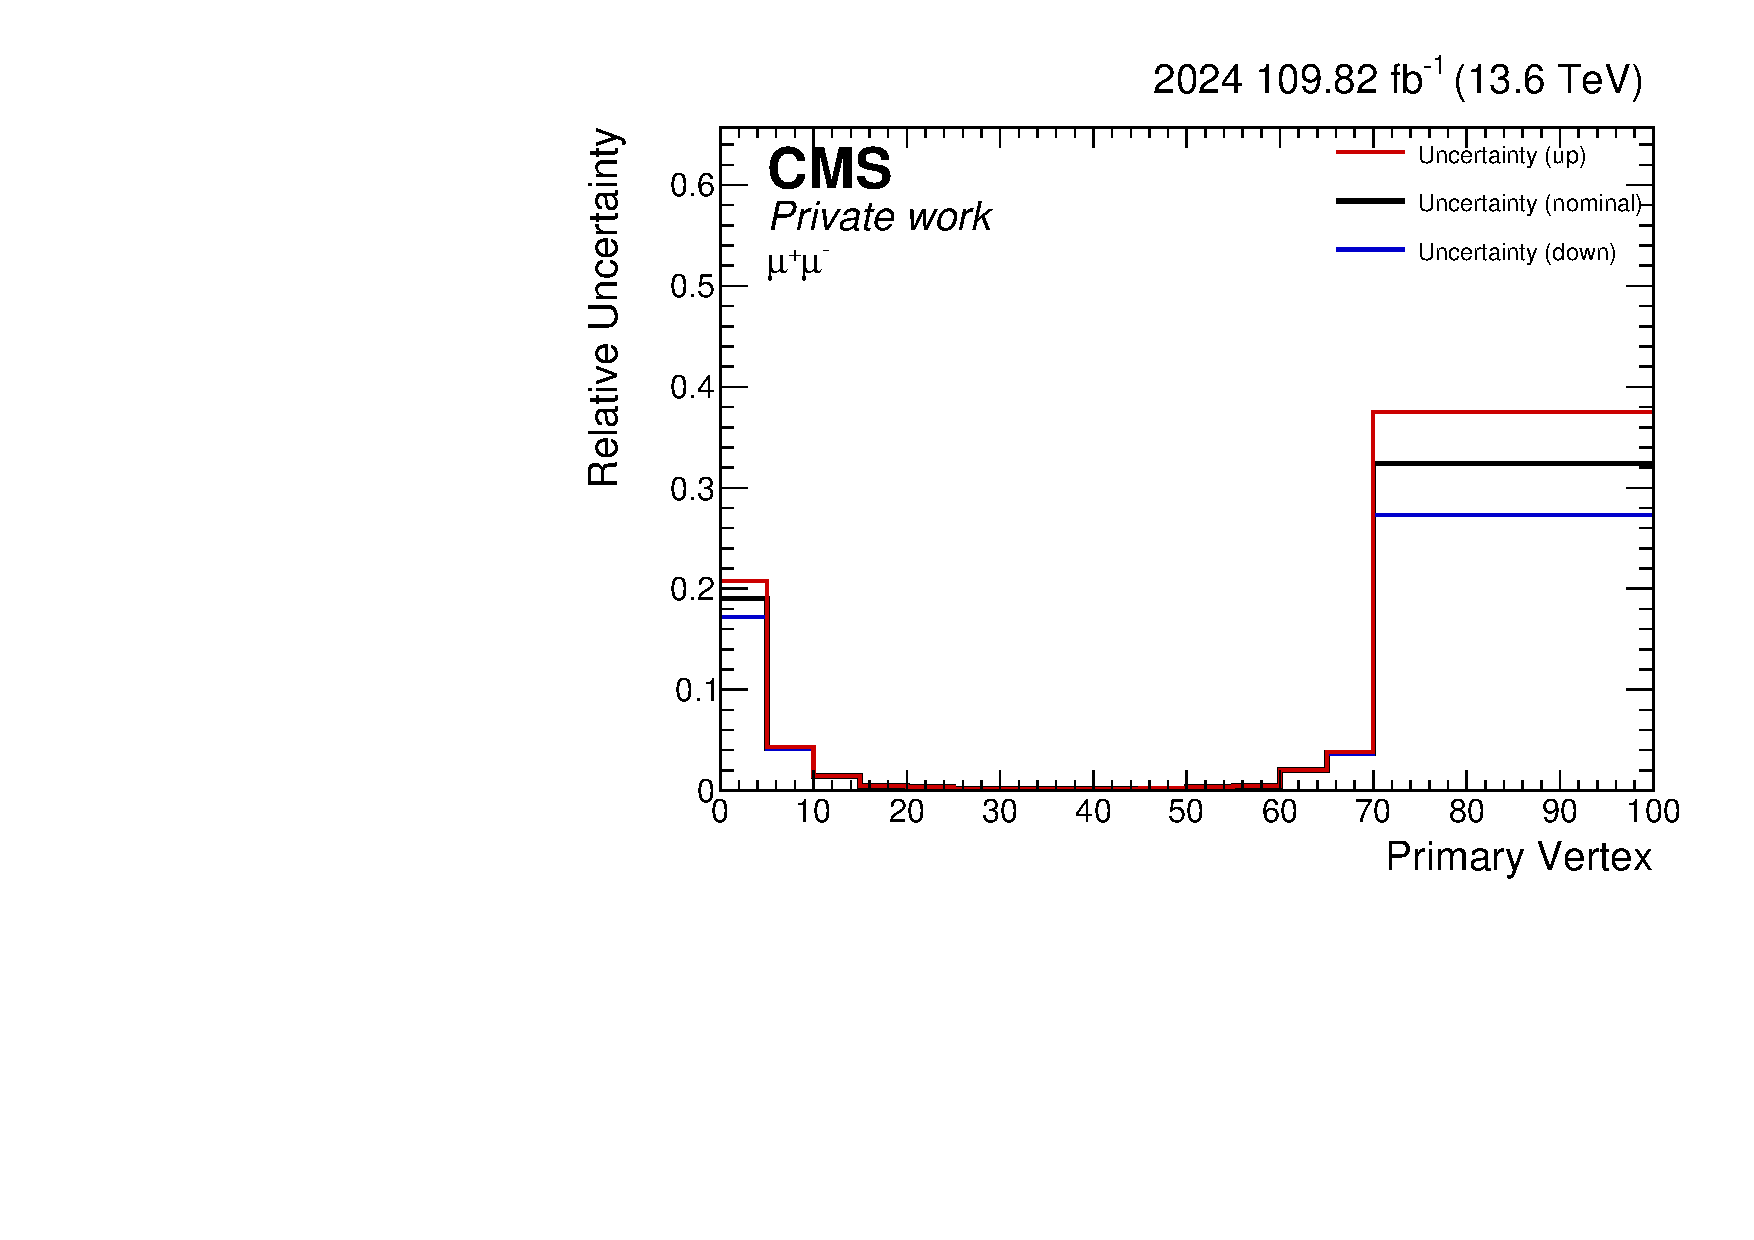
\includegraphics[width=0.48\linewidth]{figures/2024/MuMu/Statistical_Uncertainty/UncRatio_Num_PV.pdf}
\caption{Relative statistical uncertainty diagnostics, retaining the nominal, upward, and downward curves of the supplied production in the $\mu\mu$ channel. Left and right: jet and primary-vertex multiplicities.}\label{fig:extra-MuMu-Statistical-Uncertainty-Num_Jets}\end{figure}
\begin{figure}[p]\centering
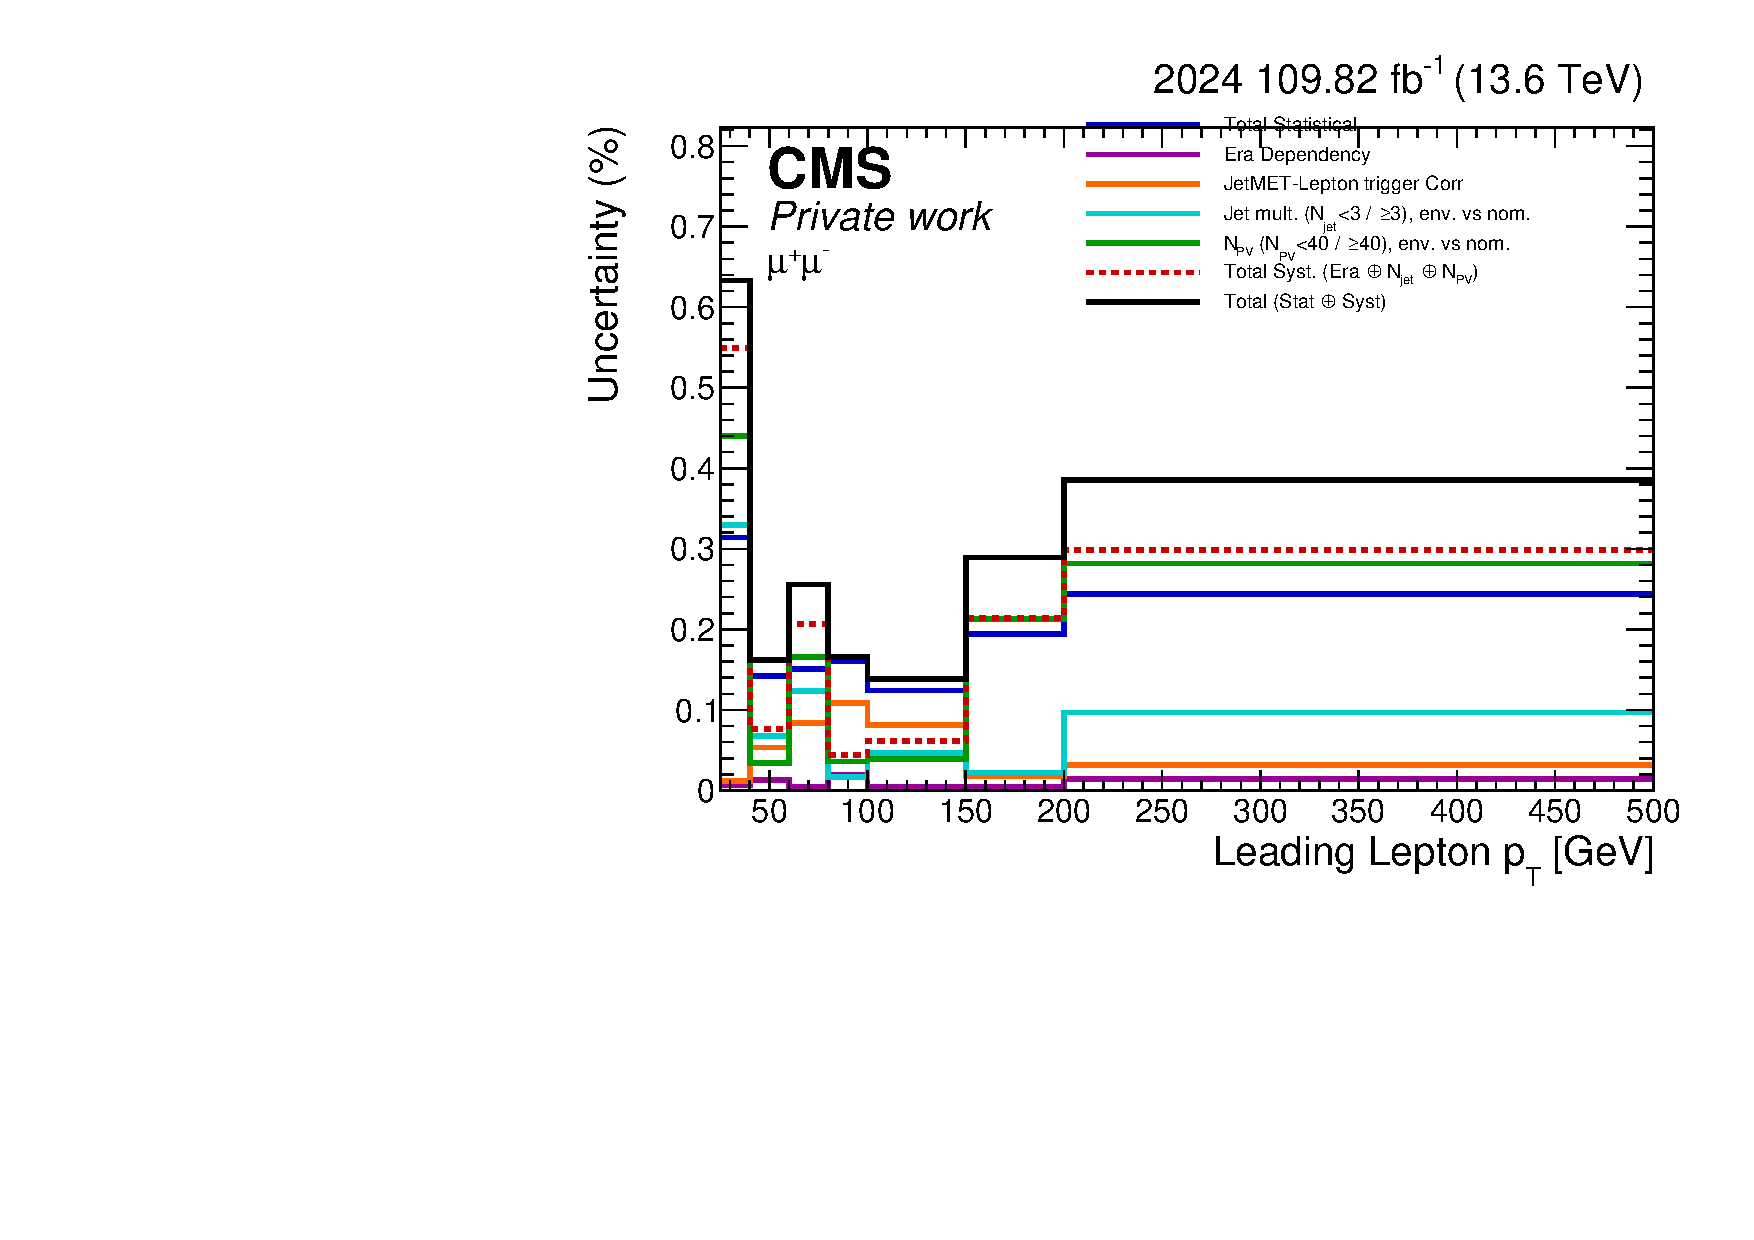
\includegraphics[width=0.48\linewidth]{figures/2024/MuMu/Uncertainty_Breakdown/Breakdown_Lep1pt.pdf}
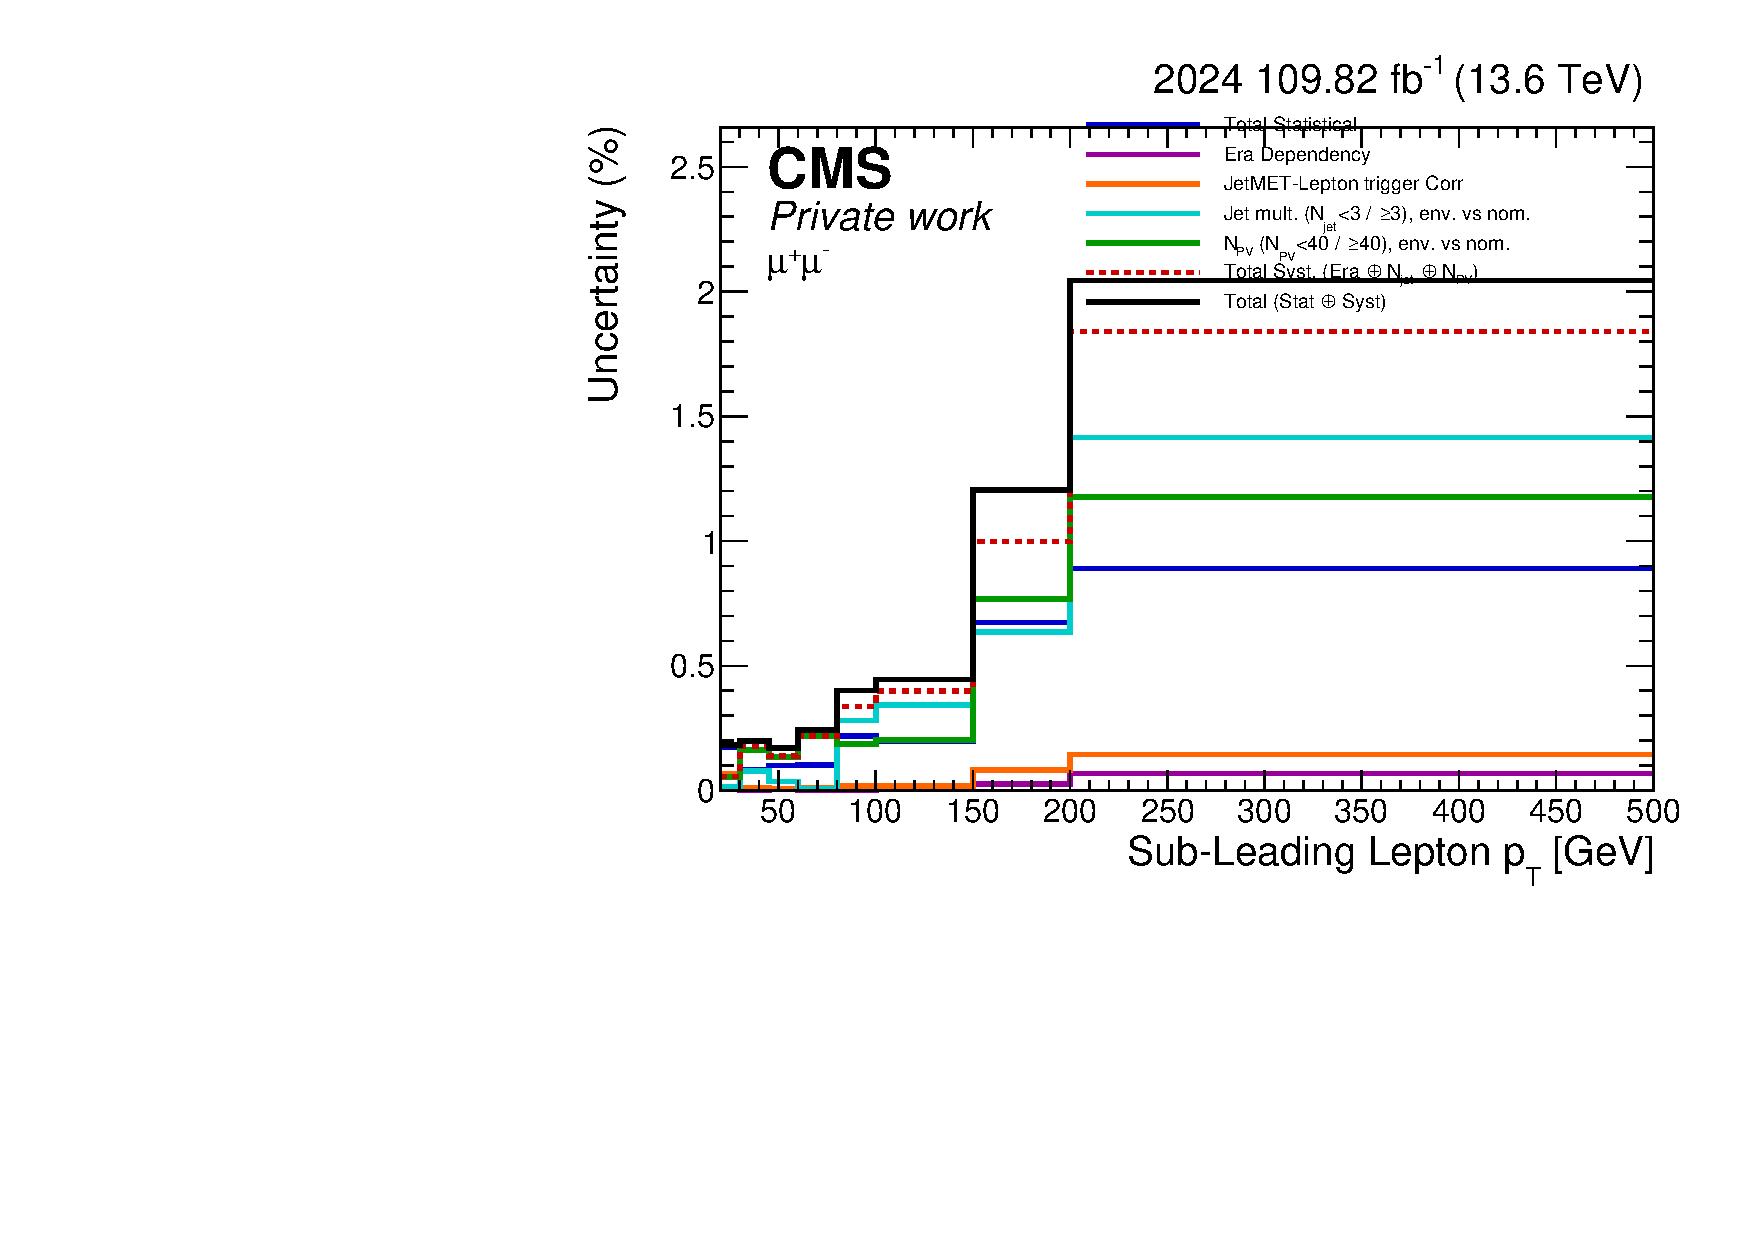
\includegraphics[width=0.48\linewidth]{figures/2024/MuMu/Uncertainty_Breakdown/Breakdown_Lep2pt.pdf}
\caption{Absolute uncertainty component breakdown in the $\mu\mu$ channel. Left and right: leading and subleading lepton $p_{\mathrm{T}}$.}\label{fig:extra-MuMu-Uncertainty-Breakdown-Lep1pt}\end{figure}
\begin{figure}[p]\centering
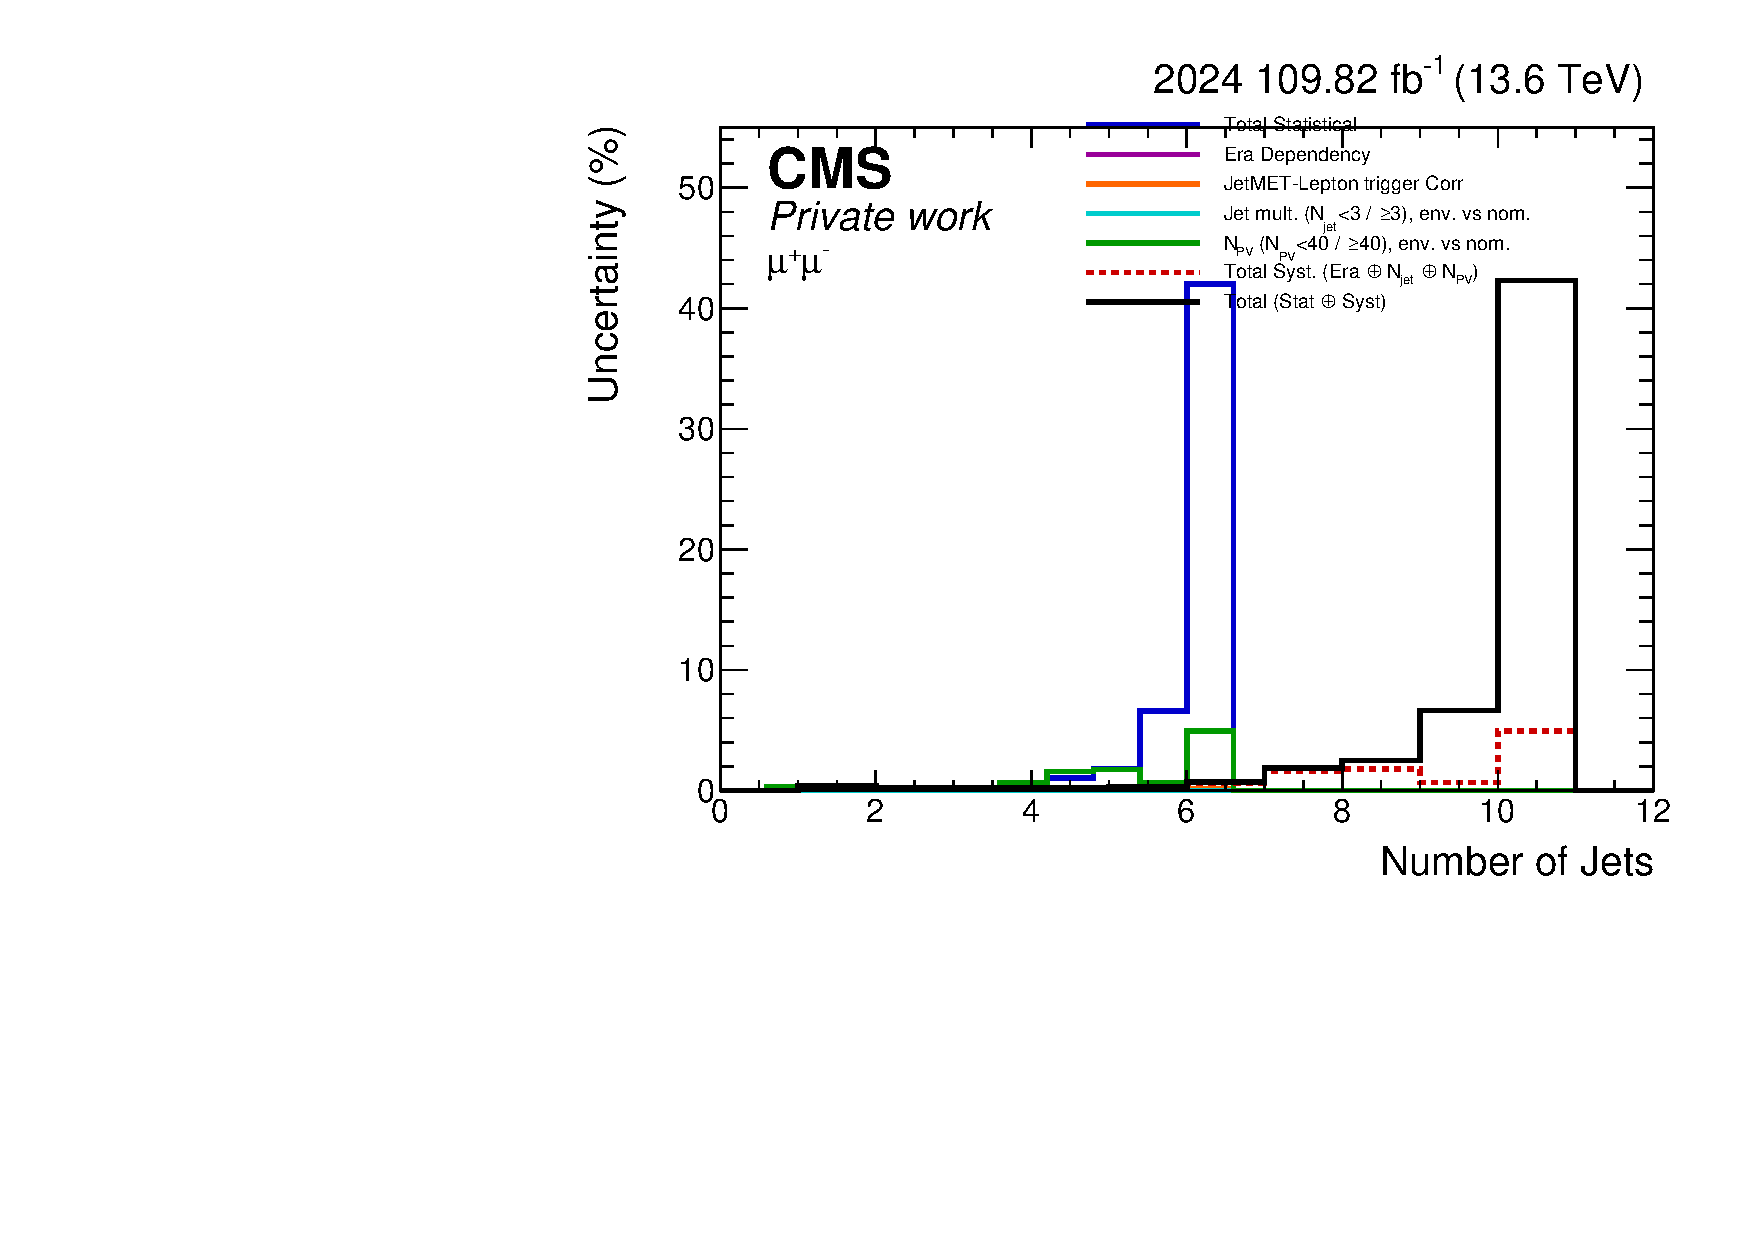
\includegraphics[width=0.48\linewidth]{figures/2024/MuMu/Uncertainty_Breakdown/Breakdown_Num_Jets.pdf}
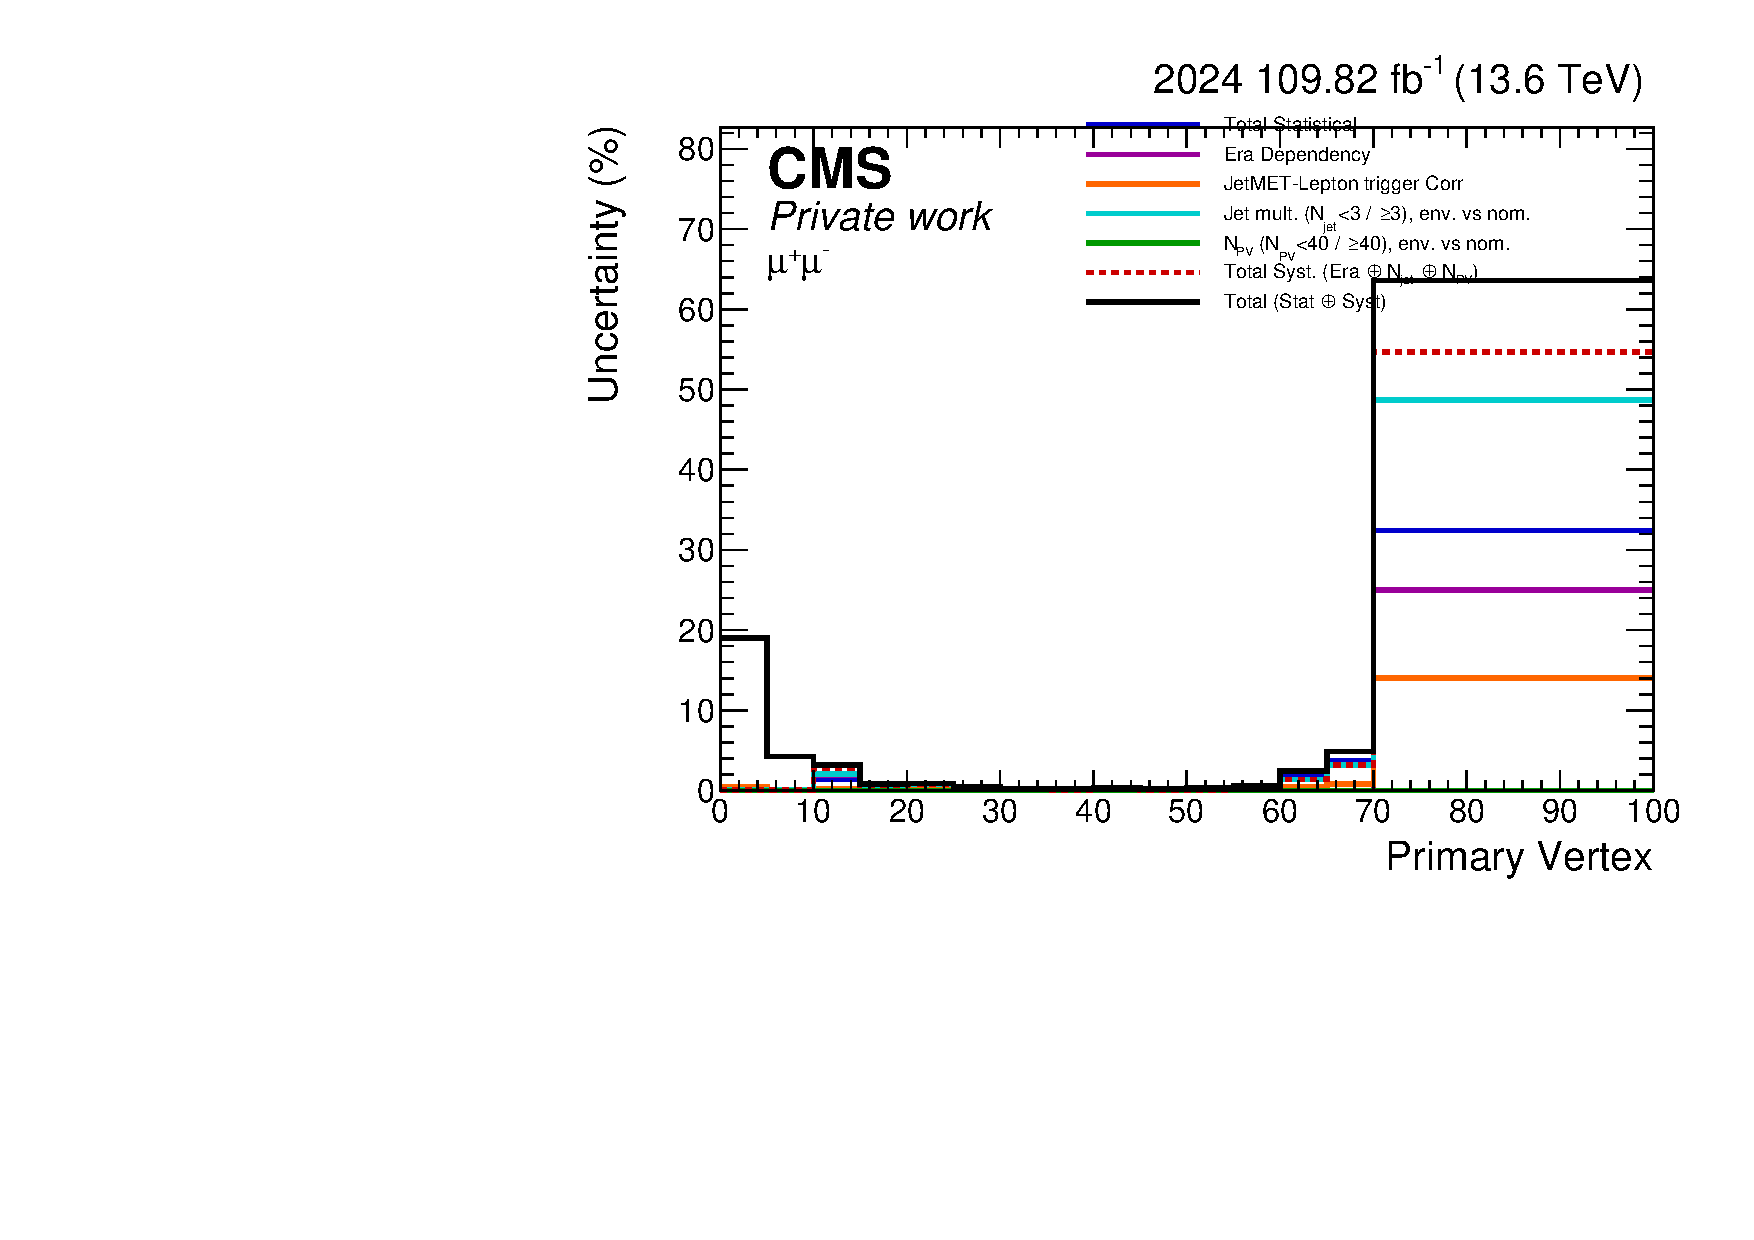
\includegraphics[width=0.48\linewidth]{figures/2024/MuMu/Uncertainty_Breakdown/Breakdown_Num_PV.pdf}
\caption{Absolute uncertainty component breakdown in the $\mu\mu$ channel. Left and right: jet and primary-vertex multiplicities.}\label{fig:extra-MuMu-Uncertainty-Breakdown-Num_Jets}\end{figure}
\begin{figure}[p]\centering
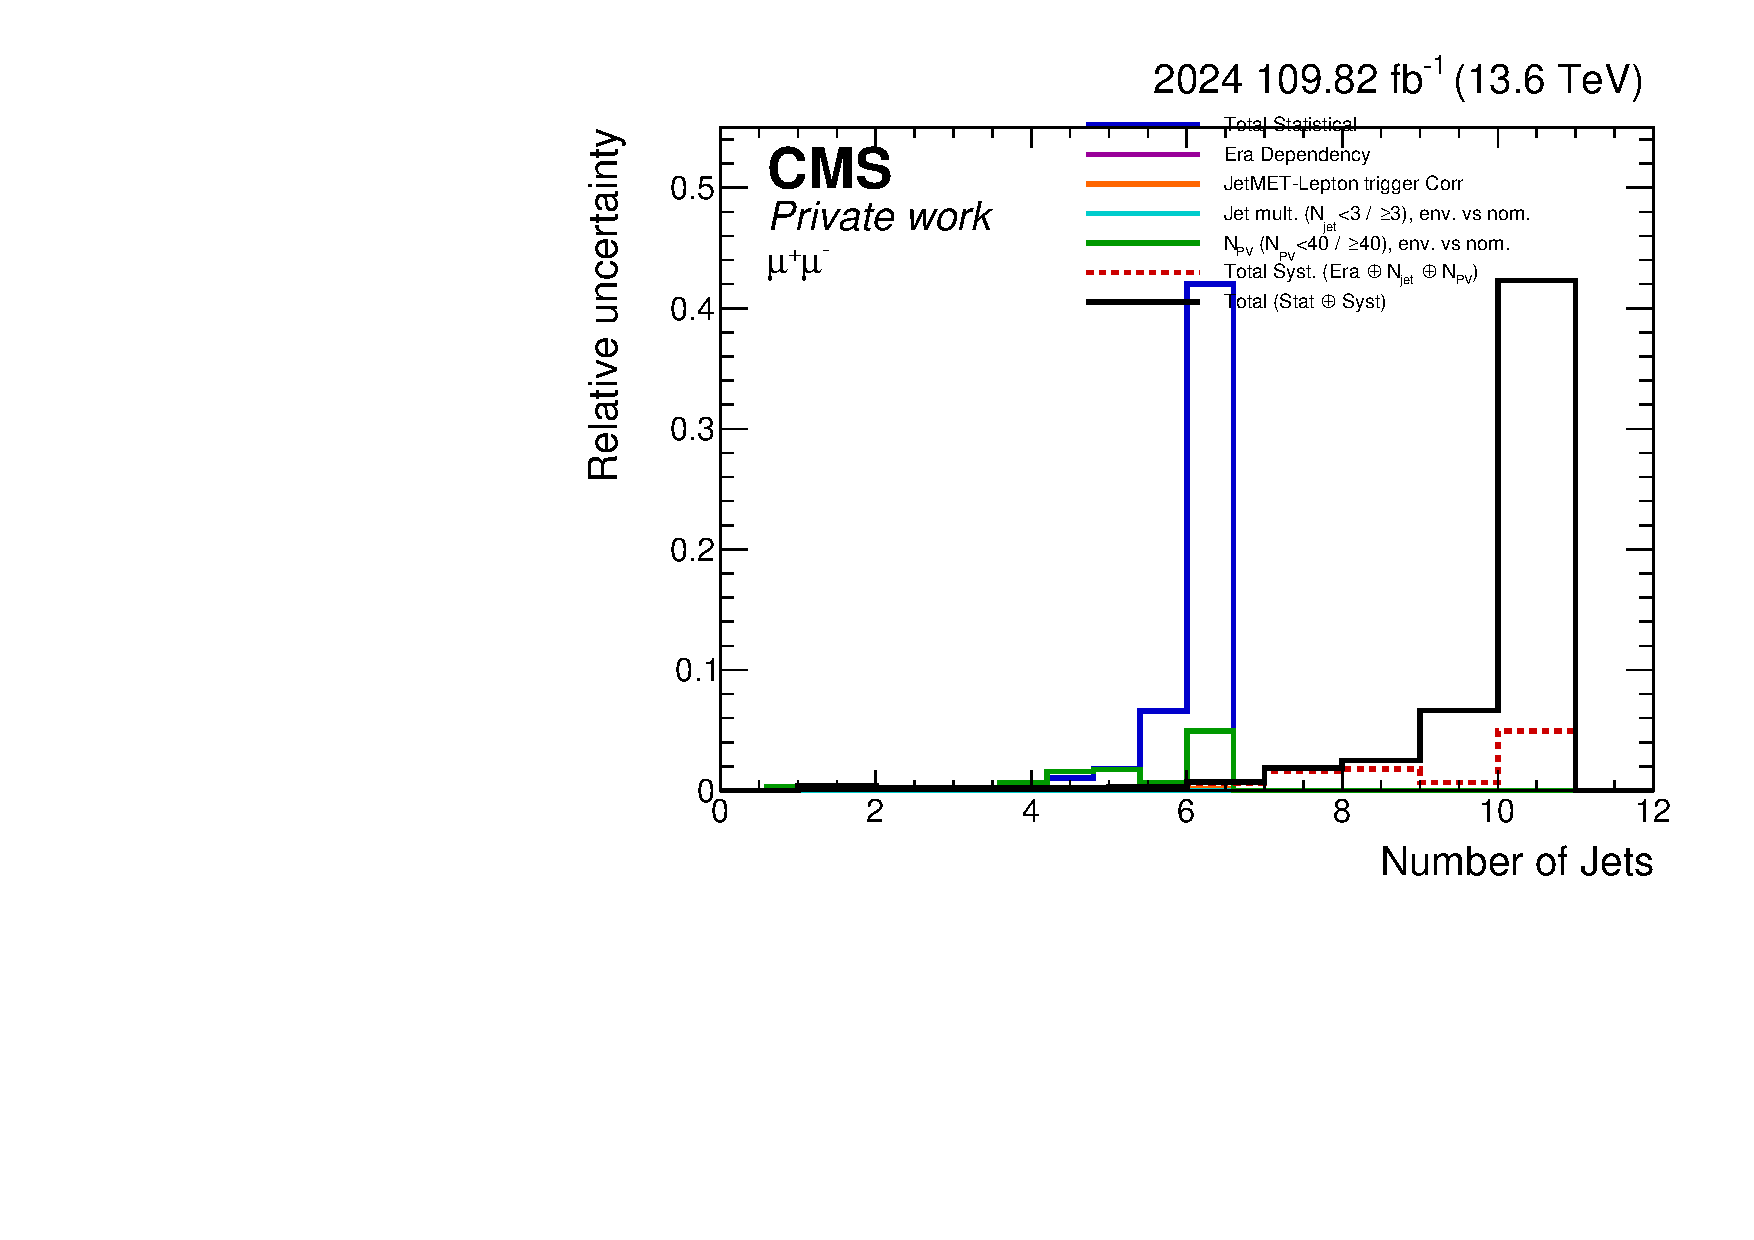
\includegraphics[width=0.48\linewidth]{figures/2024/MuMu/Relative_Uncertainty_Breakdown/Breakdown_Num_Jets.pdf}
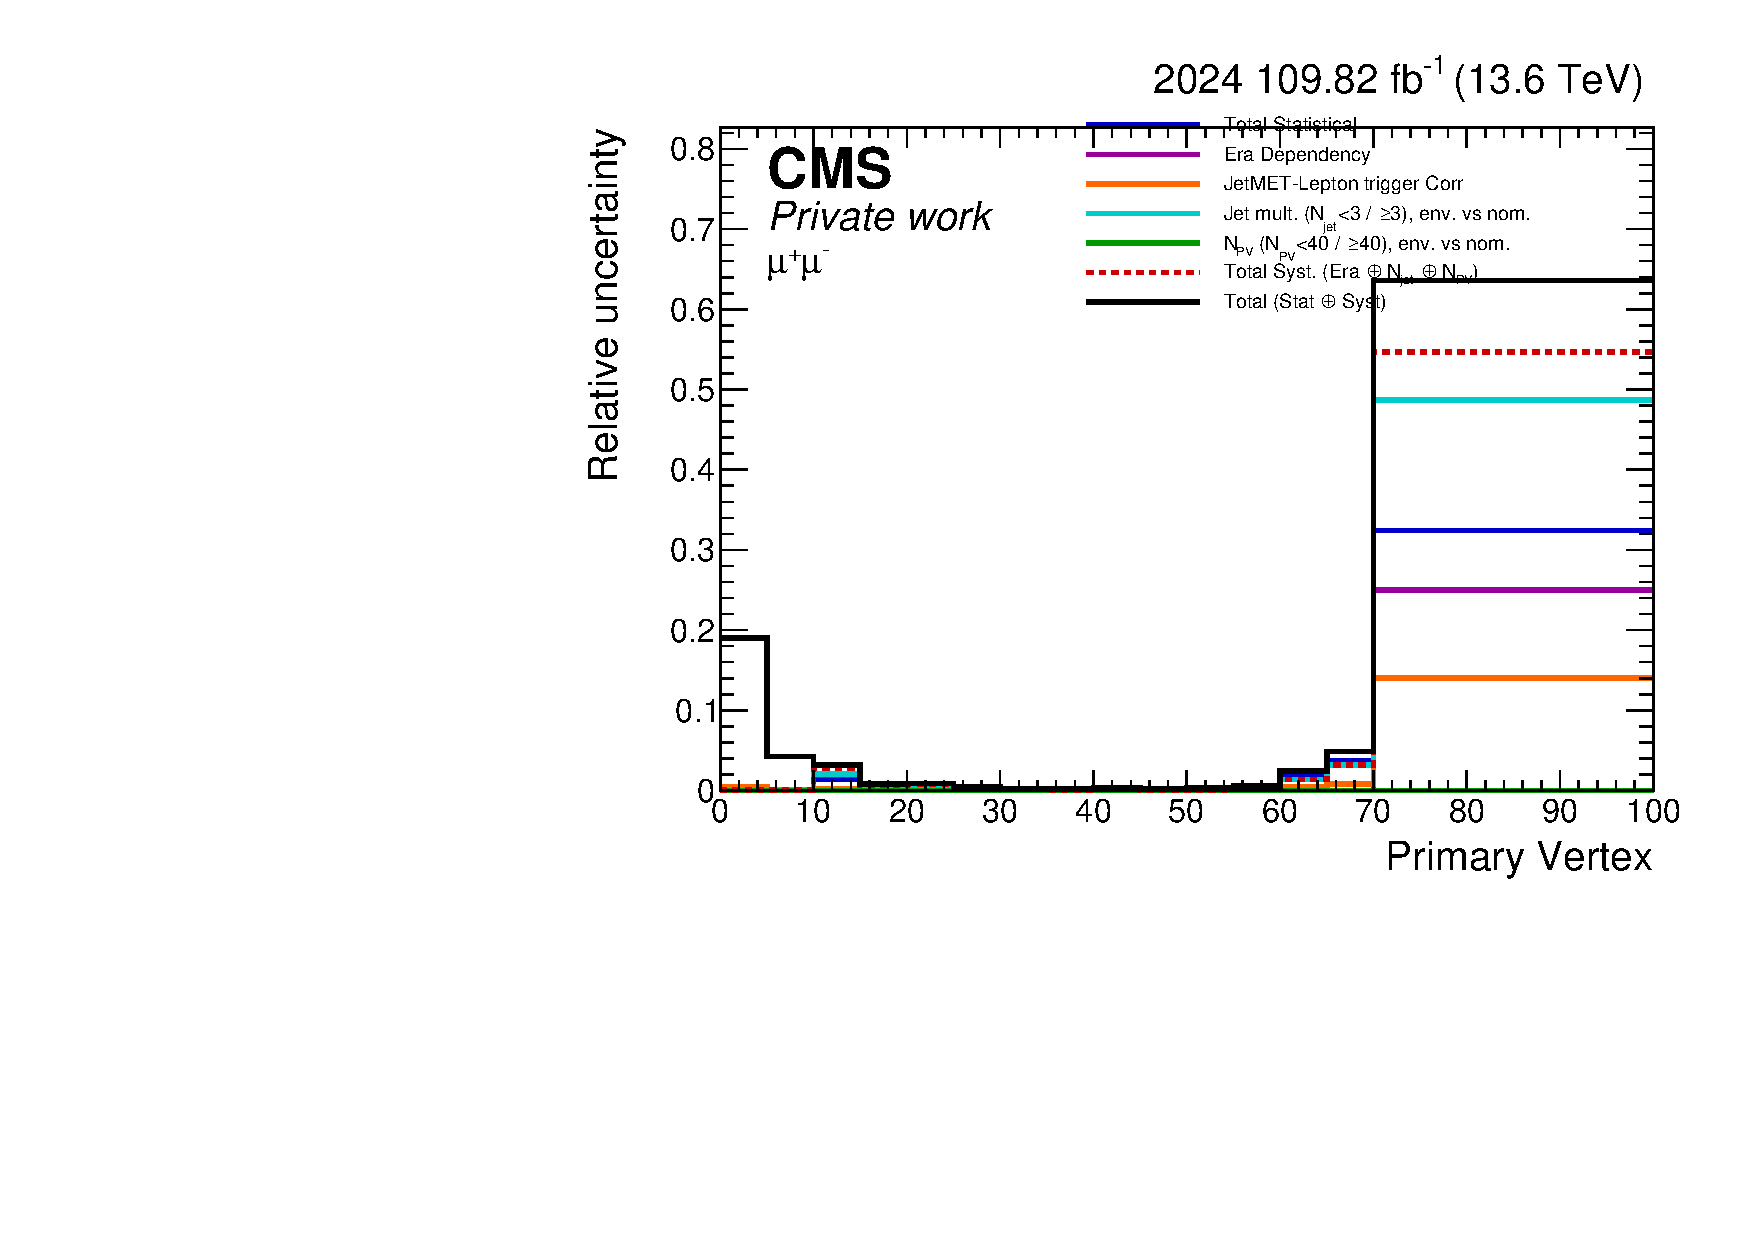
\includegraphics[width=0.48\linewidth]{figures/2024/MuMu/Relative_Uncertainty_Breakdown/Breakdown_Num_PV.pdf}
\caption{Relative uncertainty component breakdown versus event activity in the $\mu\mu$ channel. Left and right: jet and primary-vertex multiplicities.}\label{fig:extra-MuMu-Relative-Uncertainty-Breakdown-Num_Jets}\end{figure}
\begin{figure}[p]\centering
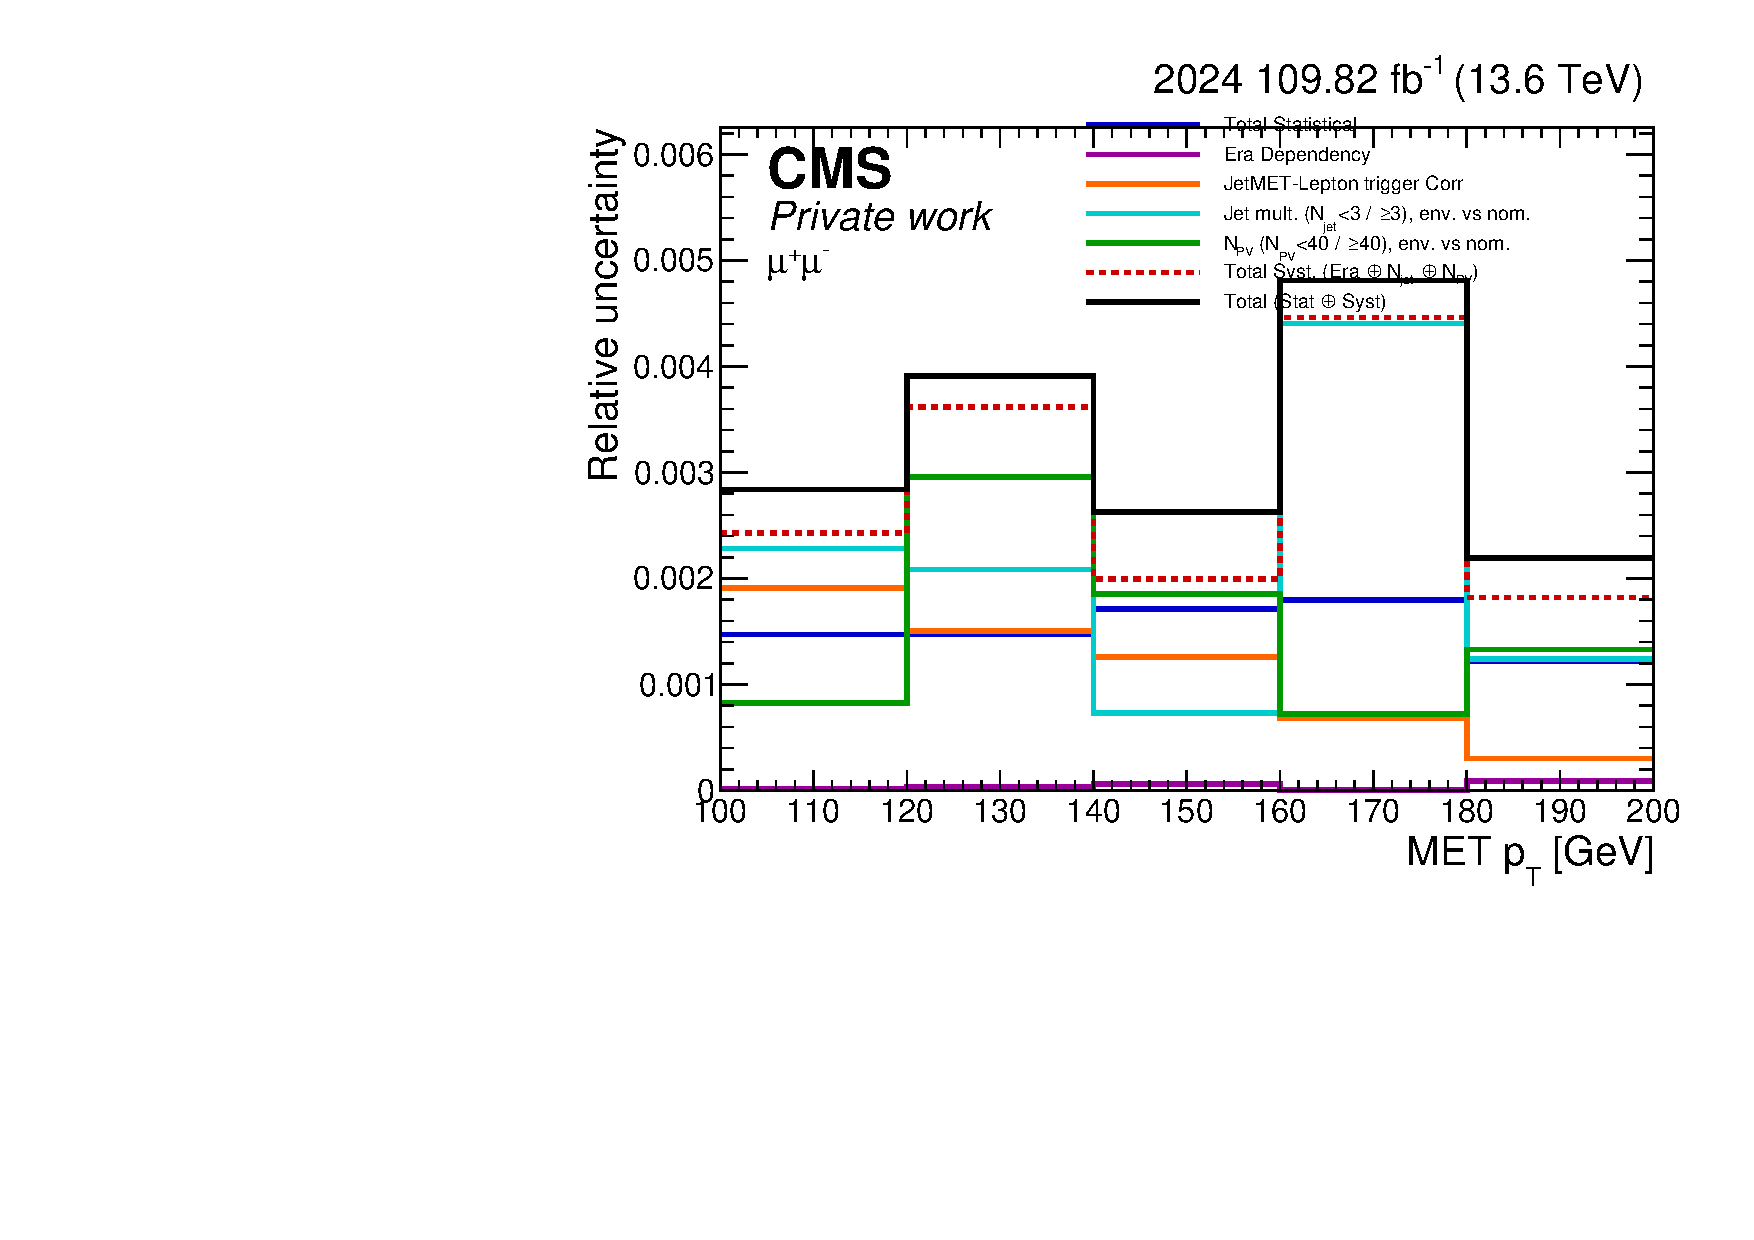
\includegraphics[width=0.48\linewidth]{figures/2024/MuMu/Relative_Uncertainty_Breakdown/Breakdown_METpt.pdf}
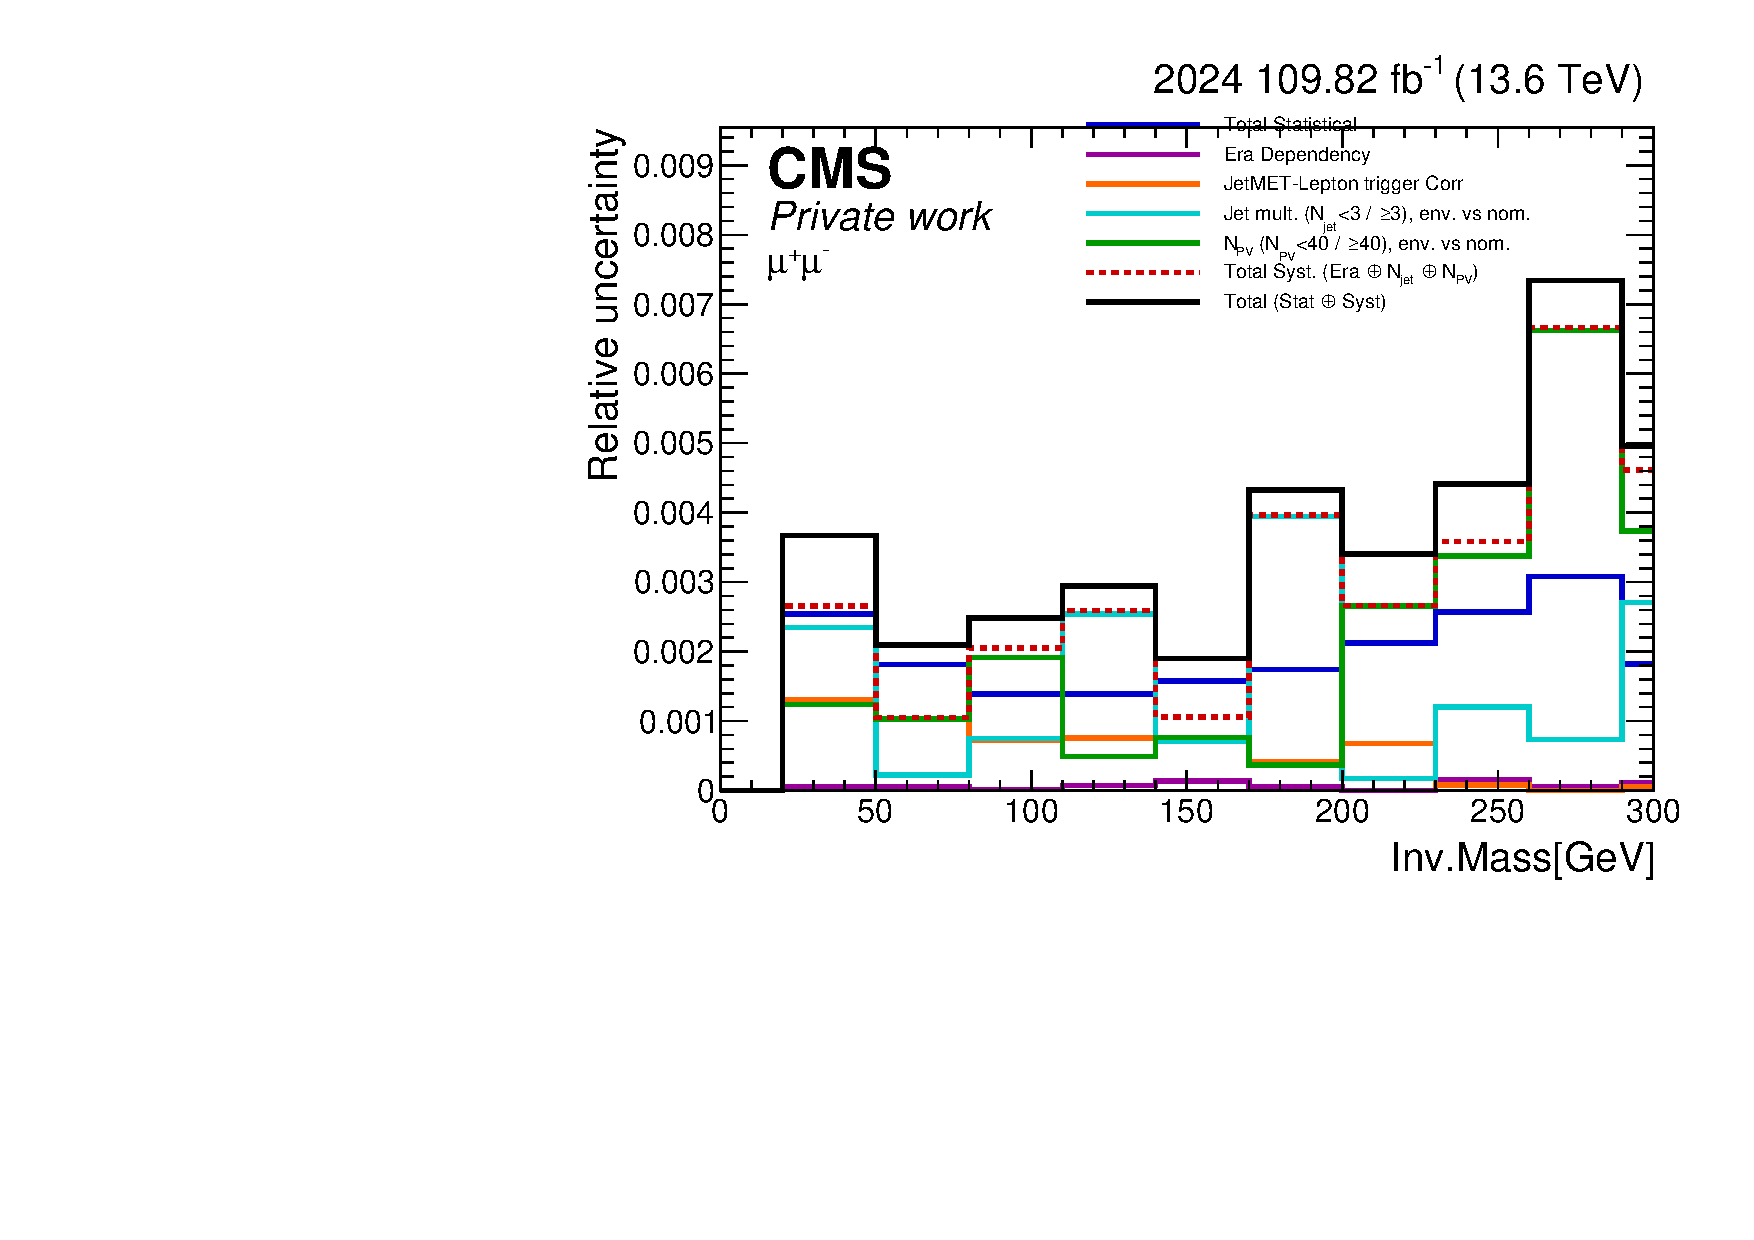
\includegraphics[width=0.48\linewidth]{figures/2024/MuMu/Relative_Uncertainty_Breakdown/Breakdown_DiLepMass.pdf}
\caption{Relative uncertainty component breakdown versus event kinematics in the $\mu\mu$ channel. Left and right: missing transverse momentum and dilepton invariant mass.}\label{fig:extra-MuMu-Relative-Uncertainty-Breakdown-METpt}\end{figure}
\begin{figure}[p]\centering
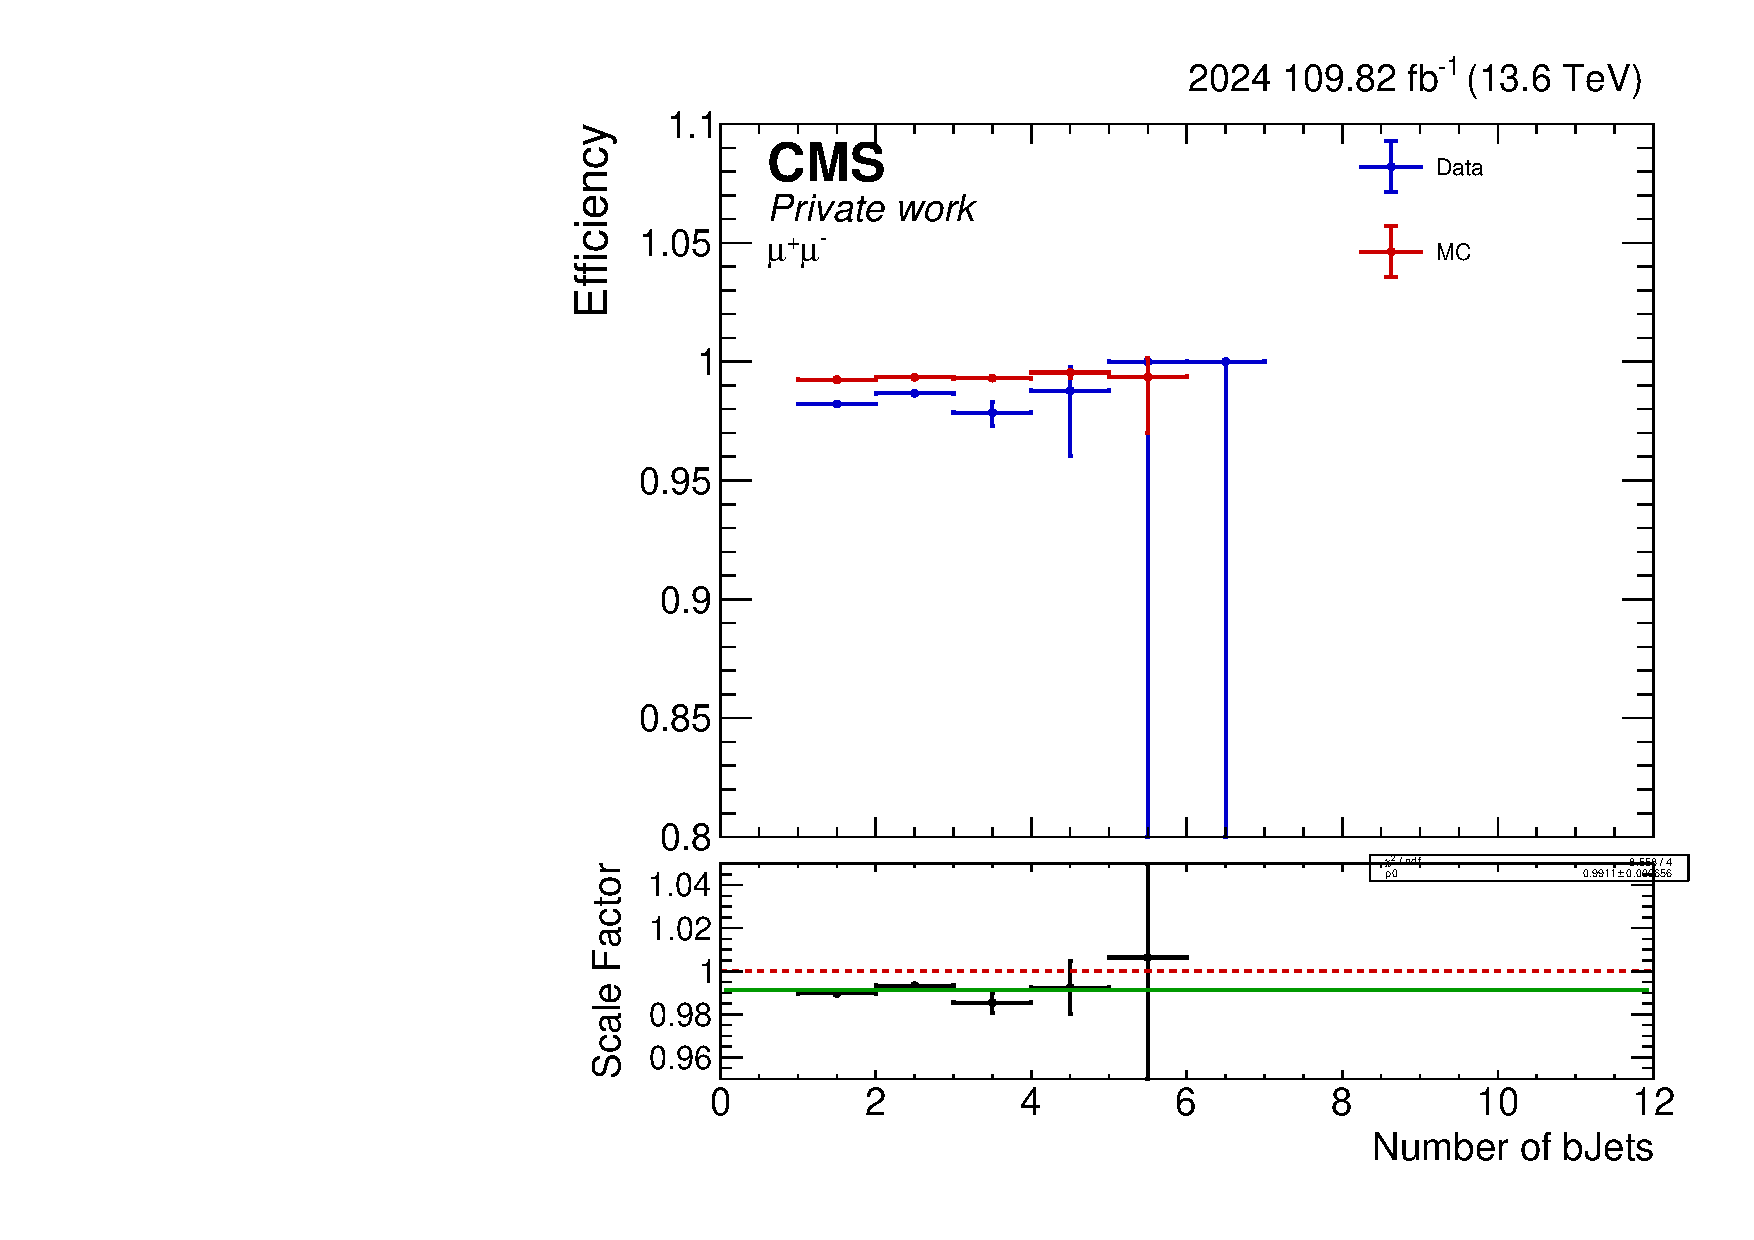
\includegraphics[width=0.48\linewidth]{figures/2024/MuMu/ScaleFactor/SF_Num_bJets.pdf}
\caption{Efficiency comparison and scale factor versus heavy-flavour activity in the $\mu\mu$ channel. $b$-tagged jet multiplicity.}\label{fig:extra-MuMu-ScaleFactor-Num_bJets}\end{figure}
